\documentclass[10pt,a4paper]{article}
\usepackage[utf8]{inputenc}
\usepackage[czech]{babel}
\usepackage[top=1cm, bottom=2cm, left=1cm, right=1cm]{geometry}
%\usepackage[margin=1.2cm]{geometry}
\usepackage{graphicx}
\usepackage{multirow}
\usepackage{tabulary}
\usepackage{tocloft}% http://ctan.org/pkg/tocloft
\usepackage{listings}
\usepackage{xcolor}
\usepackage[unicode]{hyperref}
\usepackage{mathtools}
\usepackage{amssymb}
\usepackage{tikz}
\makeatletter
\renewcommand*\env@matrix[1][*\c@MaxMatrixCols c]{%
  \hskip -\arraycolsep
  \let\@ifnextchar\new@ifnextchar
  \array{#1}}
\makeatother
\setlength{\cftsubsecnumwidth}{3em}% Set length of number width in ToC for \subsection
\setlength{\cftsubsubsecnumwidth}{4em}% Set length of number width in ToC for \subsubsection
\author{}
%\author{Richard Zvonek}
\title{Vypracované otázky ke státní závěrečné zkoušce \\VŠB-TUO FEI}

\begin{document}


\maketitle
\begin{center}
\large{DISCLAIMER:}\\
Tento dokument byl vytvořen téměř výhradně za pomocí následujících webových stránek: 
\begin{enumerate}
\centering
\item \url{http://szz.kajfosz.cz/}
\item \url{http://lucie.zolta.cz/}
\end{enumerate}
Drtivá většina textu byla z těchto stránek převzata.\\
Aktuální verze tohoto dokumentu je dostupná zde:\\ \url{https://www.overleaf.com/read/vhjnptstqcxf}
\end{center}
\newpage
\tableofcontents
\newpage
\part{Informační a komunikační technologie}
\newpage
\section{Logické obvody}
\subsection{Booleova algebra, Booleovské funkce a vazba na kombinační obvody}
Booleova algebra je binární algebra (má jen dvě konstanty 0 a 1) a využívá tři základní operace:
\begin{itemize}
\item Negace - NOT
\item Logický součin - AND
\item Logický součet - OR
\end{itemize}
Pomocí Booleovy algebry můžeme minimalizovat logické funkce dle daných zákonů a pravidel:

\begin{itemize}
\item Komutativní: $a + b = b + a$
\item Asociativní: $a + (b + c) = (a + b) + c$
\item Distributivní: $a \times (b + c) = (a \times b) + (a \times c)$
\item Indepotentní:
\begin{itemize}
\item $a + a = a$
\item $a \times a = a$
\item $a + 1 = 1$
\item $a \times 1 = a$
\item $a + 0 = a$
\item $a \times 0 = 0$
\end{itemize}

\end{itemize}

Pro vyjádření pravdivostních hodnot logických funkcí existuje několik metod.


\begin{itemize}
\item Rovnice / předpis funkcí
\begin{itemize}
\item $P = a \times b \times c$
\item P nabude stavu log 1 když budou všechny proměnné $(a,b,c)$ ve stavu log 1
\end{itemize}
\item Pravdivostní tabulka
\item Karnaughova mapa
\item Grafický zápis pravdivostní tabulky, kde každému řádku odpovídá nějaké políčko ($2^N$ políček, kde $N$ je počet proměnných)
\end{itemize}


\subsection{Zobrazování celých čísel a odpovídající aritmetika (dvojkový doplněk, kód s posunutou nulou (offset binary), BCD kód}
\begin{itemize}
\item Celá čísla (Z) se skládají z kladných i záporných čísel, včetně 0.
\item Problém tedy je pomocí bitů vyjádřit jak kladná tak záporná čísla $\rightarrow$ bit s největší váhou (most left) tedy označuje jestli se jedná o kladné číslo (0) nebo o záporné (1).
\item Nevýhoda je, že máme dva stavy i pro nulu, záporná a kladná nula.
\item Komplikuje aritmetické operace $\rightarrow$ jsou potřeba odlišné algoritmy pro kladná a záporná čísla
\item Tato metoda se nazývá Přímý kód
\end{itemize}

\subsubsection{Dvojkový doplněk}
\begin{itemize}
\item Dvojkový doplňkový kód je nejrozšířenějším způsobem reprezentace celých čísel se znaménkem v počítači.
\item Způsob kódování celých čísel tak, že ALU používá stejné aritmetické algoritmy pro kladné/záporné čísla, ale jinak je čte.
\item Odstraňuje problém s kladnou a zápornou nulou
\item Odečítání se realizuje jako: první číslo + dvojkový doplněk druhého čísla
\item Při použití dvojkového doplňku se opačné číslo získá tak, že se znegují všechny bity čísla a k výsledku se přičte jednička
\item Příklad:
\item 0111 nebo-li číslo 7
\item provedeme negaci bitů: 1000
\item Přičteme 1: 1001 a máme -7
\end{itemize}

\subsubsection{Kód s posunutou nulou (offset binary)}
\begin{itemize}
\item k číslu připočítáváme nějakou známou konstantu kterou si stanovíme.
\item většinou se jedná o konstantu v půlce intervalu. Např. pro 8bitové čísla, která mohou nabývat 256 hodnot, zvolíme hodnotu 128 (10000000).
\item K číslu, které pak chceme znázornit přičteme stanovenou konstantu.
\item Kladné čísla pak mají na začátku 1 a záporné 0. (naopak než přímý kód!, vyplývá to z výpočtu)
\item Nevýhodou tohoto zápisu je, že kladná čísla se liší od bezznaménkové reprezentace čísel.
\end{itemize}

\subsubsection{Binary Coded Decimal (BCD) kód}
\begin{itemize}
\item způsob kódování celých čísel s využitím pouze desítkových číslic (0-9) v jednom nibblu (4bity)
\item existuje $2^4$(16) kombinací nibblu, a desítkových číslic je jen deset, je šest kombinací nevyužito $\rightarrow$ neúsporné
\item Příklad: Číslo 29 se pomocí BCD kóduje jako "0010 1001", každá čtveřice bitů odpovídá jedné decimální číslici.
\item BCD is very common in electronic systems where a numeric value is to be displayed, especially in systems consisting solely of digital logic, and not containing a microprocessor.
\end{itemize}
\subsection{Zobrazení čísel s pevnou řádovou čárkou, aritmetika}
\begin{table}[ht]
\centering
\begin{tabular}{r|llllllll}
\hline
Pozice bitu         & 8  & 7  & 6  & 5  & 4  & 3   & 2    & 1     \\
Váha bitu           & 24 & 23 & 22 & 21 & 20 & 2-1 & 2-2  & 2-3   \\
Desítková váha bitu & 16 & 8  & 4  & 2  & 1  & 0,5 & 0,25 & 0,125 \\ 
\hline
\end{tabular}
\caption{Číslo s pevnou řadovou čárkou}
\label{tab:fixedPoint}
\end{table}

\subsection{Zobrazení čísel s pohyblivou řádovou čárkou (IEEE 754-2008, binární a decimální základ), aritmetika}
\begin{itemize}
\item Pro zobrazení velkých nebo desetinných čísel.
\item $X = S M\cdot B^E (-5.97 x 10^47)$
\begin{itemize}
\item S je znaménko
\item M je mantisa (část za desetinnou čárkou)
\item B je základ
\item E je exponent
\end{itemize}
\item Lze zobrazit v několika přesnostech

\begin{itemize}
\item Jednoduchá (32bitů)
\item Dvojnásobná (64bitů)
\item Rozšířená (80bitů)
\end{itemize}
\item Standard IEEE 754-2008 rozšířil tyto přesnosti ještě o čísla s poloviční a čtyřnásobnou přesností
\end{itemize}

\begin{table}[ht]
\centering
\begin{tabular}{r|llll}
\hline
Počítač/norma/systém & Šířka (b) & Báze & Exponent (b) & Mantisa (b) \\
\hline
IEEE 754 half        & 16        & 2    & 5            & 10+1        \\
IEEE 754 single      & 32        & 2    & 8            & 23+1        \\
IEEE 754 double      & 64        & 2    & 11           & 52+1       \\
\hline
\end{tabular}
\caption{Některé používané normy IEEE 754}
\label{tab:iee754}
\end{table}

\begin{table}[ht]
\centering
\begin{tabular}{r|r|lr|lr}
\hline
Bit & 31 & 30  & 23 &22  & 0 \\
Význam & $z^a$ & \multicolumn{2}{c}{Exponent} & \multicolumn{2}{|c}{Mantisa}    \\

\hline
\end{tabular}
\caption{Zobrazení čísla s pohyblivou řádovou čárkou dle IEE 754 signle precision}
\label{tab:floatingPoint}
\end{table}



\subsection{Kódování znaků, ASCII, Unicode}
\subsubsection{Ascii}
\begin{itemize}
\item Tabulka, která definuje znaky anglické abecedy a další znaky
\item 7bitová, tzn $2^7$ (128) znaků.
\item Dle potřeby rozšíření na 8bitů (256znaků) pro další národy než jen Amíky. Prvních 128 bitů je shodných s ASCII a zbytek doplněn o extra. Pro češtinu Windows-1250 nebo ISO 8859-2
\item Tl;dr vznikl bordel a chaos, proto Unicode
\end{itemize}


\subsubsection{Unicode}
\begin{itemize}
\item Sjednocená tabulka všech abeced různých jazyků
\item V současnosti přes 100.000 znaků, možnost až 1 114 112 znaků do budoucna.
\item Verze UTF-8, UTF-16, UTF-32, podle počtu bitů sloužícím k zakódování znaku (je to však velikost minimální, některé znaky mohou být kódovány i vyšším počtem bitů.)
\item Výhoda: obsahuje všechny znaky
\item Nevýhoda: větší velikost a náročnost kódování
\item Aktuální verze Unicode 12
\item Pro kód znaku musí být použita nejkratší možná sekvence bajtů. Počet jedničkových bitů na začátku prvního bajtu ve vícebajtové sekvenci odpovídá počtu bajtů sekvence.
\end{itemize}
\begin{table}[ht]
\centering
\begin{tabular}{l|l}
\hline
U+00000000 - U+0000007F & 0xxxxxxx                                              \\
U+00000080 - U+000007FF & 110xxxxx 10xxxxxx                                     \\
U+00000800 - U+0000FFFF & 1110xxxx 10xxxxxx 10xxxxxx                            \\
U+00010000 - U+001FFFFF & 11110xxx 10xxxxxx 10xxxxxx 10xxxxxx                   \\
U+00200000 - U+03FFFFFF & 111110xx 10xxxxxx 10xxxxxx 10xxxxxx 10xxxxxx          \\
U+04000000 - U+7FFFFFFF & 1111110x 10xxxxxx 10xxxxxx 10xxxxxx 10xxxxxx 10xxxxxx \\
\hline
\end{tabular}
\caption{Kódování znaku v UTF8}
\label{tab:utf8}
\end{table}
\subsection{Automat s konečným počtem stavů, Moore a Mealy automat}
\subsubsection{Automat s konečným počtem stavů}
\begin{itemize}
\item Nebo-li DFA $\rightarrow$ UTI
\item FSM $\rightarrow$ Finite State Machine
\item DSM $\rightarrow$ Deterministický Stavový Automat
\end{itemize}

\subsubsection{Moore}
\begin{itemize}
\item Výstup se projeví až po přechodu, tedy v dalším stavu.
\item Výstup je tedy určen pouze současným stavem.
\end{itemize}

\subsubsection{Mealy}
\begin{itemize}
\item Automat, jehož výstup je určen současným stavem a současným vstupem. 
\item Výstup není ve stavu ale při přechodu na další stav
\item Díky tomu často vyžaduje méně stavů.
\end{itemize}
\begin{table}[ht]
\centering
\begin{tabular}{rll}
\hline
                   & Moore         & Mealy                          \\
                   \hline
Výstup             & Současný stav & Současný stav a současný vstup \\
Při změně vstupu   & Beze změny    & Výstup se změní                \\
Počet stavů        & Více          & Méně                           \\
HW požadavky       & Vyšší         & Nižší                          \\
Rychlost reakce    & Nižší         & Vyšší                          \\
Výstup             & Ve stavu      & Při přechodu                   \\
Náročnost na návrh & Jednoduchý    & Složitý             \\ \hline          
\end{tabular}
\caption{Porovnání Moore a Mealy}
\label{tab:fsm}
\end{table}

\newpage
\section{Telekomunikační sítě}
\subsection{LAN a WAN sítě (Ethernet, ATM, Frame Relay)}
\subsubsection{LAN}
\begin{itemize}
\item Sítě zpravidla na jenom menším místě (jedna budova)
\item sdílení lokálních prostředků (tiskáren, dat, aplikací)
\item Z hlediska OSI RM technologie LAN využívá pouze fyzickou a spojovou vrstvu.
\item Nejrozšířenější technologie je Ethernet
\end{itemize}

\subsubsection{Ethernet} \label{sec:ethernet}
\begin{itemize}
\item Souhrn technologií pro sítě LAN.
\item Standard IEEE 802.3
\item Pojmenování dle formátu: \{Mbps$|$GbpsG\} \{Base$|$Broad\} \{seg\_{}len/100[m] $|$-medium\}. Např.: 10Base-T
\item Koax, TP, Optika.
\item U Half-Duplexu CSMA/CD (přístup k mediu)
\begin{enumerate}
\item Naslouchá, zda je medium volné.
\item Pokud je volné, tak zahájí vysílaní a naslouchá, jestli nepřichází signál od jiné stanice. Pokud, ano, došlo ke kolizi (více stanic může detekovat volné medium a začít vysílat). Ukončí vysílání a pošle jam signál.
\item Stanice čeká náhodnou dobu, než se pokusí znovu vysílat. Pokud nastane více po sobě jdoucích kolizí, doba exponenciálně roste.
\end{enumerate}
\item Existuje více verzí rámců. Nejběžnější je DIX/Ethernet II.
\end{itemize}
\begin{figure}[ht]
    \centering
    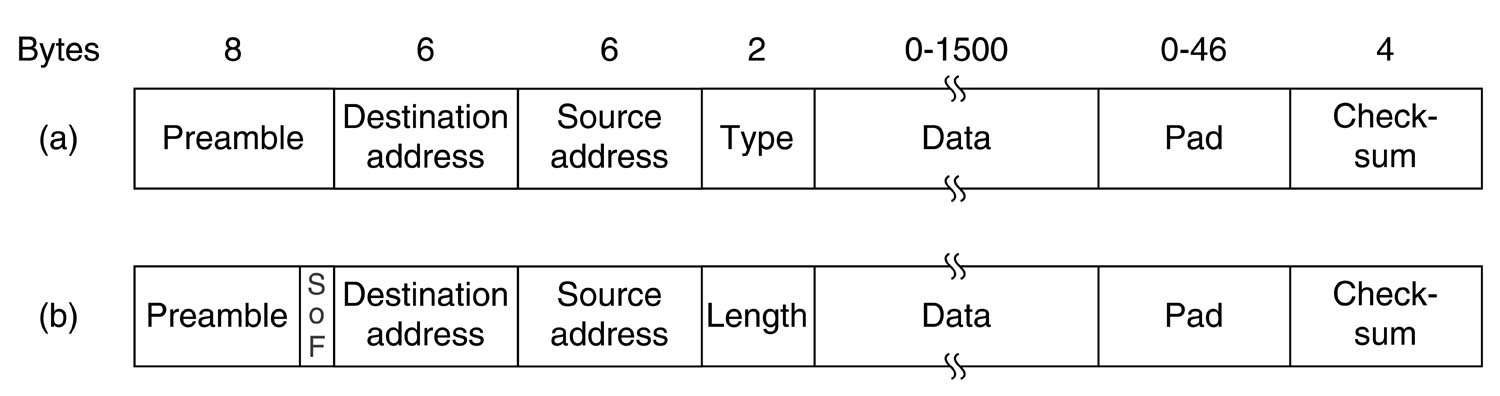
\includegraphics[width=10cm]{802frameFormat.jpg}
    \caption{Formáty rámců: (a)DIX, (b)802.3}
    \label{fig:802frameFormat}
\end{figure}
\paragraph{Základní srovnání některých variant Ethernetu}
\begin{itemize}
\item 10Base5 = Thick Ethernet - 10mm coax, až 500m dlouhé segmenty
\item 10Base2 = Thin Ethernet - 5mm coax, až 185 dlouhé segmenty
\item 10Base-T - Topologie hvězda, UTP3 kabely, dosah 100m od hubu
\item Fast Ethernet - podobné 10Base-T, 100Base-TX(UTP5), 100Base-FX(single/multi módová optická vlákna)
\item Gigabit Ethernet - 1000Base-T, 1000Base-SX
\item 10 Gigabit Ethernet - pouze full duplex(no CSMA/CD), UTP6; 10GBaseT
\end{itemize}

\subsubsection{WAN}

\begin{itemize}
\item Rozlehlejší sítě - většinou se jedná o spojení několika LAN sítí pomocí telefonních linek
\item Nejznámější WAN síť je samozřejmě Internet
\item Frame Relay

\begin{itemize}
\item Většinou trvalé virtuální spojení typu bod-bod (Permanent Virtual Circuit)
\item Možnost i SVC, které se moc nepoužívá
\item Ignoruje kontrolu a potvrzování, to přenechává vyšším vrstvám $\Rightarrow$ vyšší rychlost
\item Podporuje QOS
\item Přenos paketů zajišťuje protokol LAP-F
\item K adresaci slouží tzv. DLCI adresa
\item Dnes už se moc nepoužívá
\end{itemize}
\item ATM
\begin{itemize}
\item používá metodu virtuální cesty
\item zajišťuje QoS pro přenos hlasu a videa
\item data přenášena pomocí ATM buněk na rozdíl od rámců
\item Využívá transportní síť SDH/SONET
\item Protokolový model odpovídá prvním 4 vrstvám OSI
\end{itemize}
\end{itemize}

\subsection{Transportní sítě (SDH, DWDM, MPLS)}
Slouží k vytváření typu bod-bod
\subsubsection{SDH}

\begin{itemize}
\item Snaha zlepšit/zrychlit PDH $\Rightarrow$ synchronní přenos přes optiku
\item definován na fyzické vrstvě OSI
\item Využívá časový multiplexing
\item V USA je to SONET
\item Přenáší data a hlas přes virtuální kontejnery, do kterých jdou dát různé věci, např. ATM buňku
\item Hlavní zařízení sítě je multiplexor - terminálový a add/drop. Terminálový shlukuje kanály do 1 a add/drop přidává a odebírá data kanálů do agregovaného toku.
\item používá optické regenerátory - signál se obnoví převedením na elektrické signály a zpět na optické.
\end{itemize}
\subsubsection{DWDM}
\begin{itemize}
\item Na rozdíl od SDH se zde používá multiplexing na bázi vlnových délek
\item Používá mnoho různých vlnových délek v oblasti 1550 nm.
\item Vychází z WDM zhuštěním vlnových délek (zmenšením rozestupů
\item Každá vlnová délka = kanál o rychlosti 10Gb/s, experimentálně až 100gb/s/kanál o.O.
\item podobná zařízení jako u SDH, terminálový a add/drop multiplexor + optický cross-connector
\item na rozdíl od SDH používá vláknové zesilovače, které na rozdíl od regenerátorů nepotřebují převod na elektrické signály, ale pracují přímo s optickým signálem.
\end{itemize}

\subsubsection{MPLS}
\begin{itemize}
\item Integrace IP a virtuálních kanelů
\item Hlavní zařízení LSR - Label Switch Router, který hraje roli klasického směrovače a přepínače virtuálních kanálů.
\item Protokol který to zajišťuje je LDP, který vytváří virtuální cestu LSP z jednoho LERu do druhého. LER (Label switch Edge Router) je LSR na hranicích MPLS sítě.
\end{itemize}

\subsection{Internet, Bezpečné transportní služby (VPN, IPsec, SSL)}
Základem internetu jsou dvě služby - Webová služba + Internetová transportní síť
Internet je nejrozsáhlejší síť na světě, nefunguje podle jednotných pravidel, ale nabízí stejné služby všem uživatelům. Je to vlastně síť sítí, přičemž každá z těchto dílčích sítí je spravována jiným operátorem - ISP - Internet Service Provider.

Klasifikace internetu odpovídá klasifikaci ISP providerů. Existují dva druhy klasifikace:

\begin{enumerate}
\item
\begin{itemize}
\item Páteřní ISP - mezinárodní operátoři vlastnící sítě pokrývající určitou zemi, kontinent, nebo celý svět
\item Regionální ISP - poskytují služby v rámci určitého regionu
\item Lokální ISP - rámec malého území, např. město
\end{itemize}
\item 
\begin{itemize}
\item Tier 1 - odpovídá páteřnímu
\item Tier 2 - poskytuje služby KONCOVÝM zákazníkům v celém státě, či kontinentu
\item Tier 3 - odpovídá regionálnímu
\item Tier 4 - odpovídá lokálnímu
\end{itemize}
\end{enumerate}

Rovněž se dá klasifikovat více druhů providerů např. Internet Content Provider (ICP), Content Distribution Provider (CDP), Hosting provider a Application Service Provider (ASP)
\subsubsection{Bezpečné transportní služby}
umožňují zabezpečený přenos dat přes veřejnou síť - internet.
\paragraph{IPSec}

\begin{itemize}
\item Pracuje na \textbf{Síťové vrstvě}
\item Zabezpečuje datovou komunikaci v sítích IP
\item Autentizace, Integrita a důvěrnost dat $\leftarrow$ užívá šifrování
\end{itemize}
\paragraph{SSL/TLS}

\begin{itemize}
\item Pracuje na \textbf{prezentační vrstvě} OSI RM - zabezpečuje data aplikací/protokolů aplikační vrstvy.
\item Velmi univerzální protokoly - musí být použitelné pro velké spektrum aplikací
\end{itemize}
\paragraph{VPN}

\begin{itemize}
\item Snaží se dosáhnout vlastností skutečných privátních sítí
\item Samotná síť není fyzicky oddělena od ostatních sítí
\item Více druhů klasifikací
\begin{itemize}
\item Customer vs Provider VPN (CPVPN vs PPVPN) - o vybudování a správu se stará klient sám, nebo provider
\item Customer edge based VPN vs Provider edge based - tzn zařízení poskytující VPN je na straně zákazníka, nebo providera
\item Šifrování dat vs Oddělení provozu - IPsec VPN, SSL VPN vs MPLS VPN, ATM VPN = zabezpečené šifrované kanály vs trvalé virtuální kanály

\end{itemize}
\item Dva druhy technologií:
\begin{itemize}
\item Šifrování dat - zabezpečený kanál s IPsec, SSL
\item Oddělení provozu - dvě koncové zařízení mají svůj vlastní virtuální kanál, netřeba tak šifrovat.
\end{itemize}
\end{itemize}
\subsection{Signalizace v telekomunikačních sítích}
Signalizace se užívá pro výstavbu a pro rozpad spojení mezi ústřednami a při využívání služeb sítě.
\subsubsection{CCS7}

\begin{itemize}
\item Common Channel Signaling System No. 7
\item Spojení budováno na základě čísla volaného
\item Vysoká spolehlivost, mezinárodní norma, automatizace
\item Používá se samostatný kanál obsahující více užitečných kanálů, které jsou určeny výlučně pro komunikaci mezi uživateli
\item Kanál je navázán mezi jednotkami nazývanými SP = Signalisation point = Signalizační bod
\item STP (transfer point) jsou signalizační tranzitní body, které pouze přeposílají signály k dalšímu STP či koncovému SP
\item SCP (control point) zajišťují kontrolu a např databáze potřebné k směrování
\item Signalizační trasa = dva protisměrné kanály, všechny trasy mezi dvěma SP = signalizační spojení
\item Provoz může být částečně sdružený (užití STP), nebo sdružený (signalizační a hovorová trasa jsou shodné)
\end{itemize}
\subsubsection{H.323}

\begin{itemize}
\item Nejen hlasové služby, ale i přenos obrazu nebo videokonference
\item Zastřešuje velké množství dílčích protokolů:
\begin{itemize}
\item protokoly pro signalizaci a zabezpečený přenos
\item protokoly pro přenos multimediálních dat v reálném čase
\item protokoly pro zpracování hlasu a videa
\end{itemize}
\item Architektura rozdělena do Administrativních domén - kolekce komponent spravována tzv. Gatekeeperem
\item Velmi robustní a obtížný protokol na implementaci
\end{itemize}
\subsubsection{SIP}

\begin{itemize}
\item Navržený pro snadnou implementaci a rozšiřitelnost. Pracuje na aplikační vrstvě.
\item Užívá se pro sestavení, modifikaci a ukončení spojení přenosu hlasu přes Internet - VoIP
\item Ve spojení s ním se ještě užívá RTP (Real-Time Protokol, zajišťuje přenos hlasu v paketech přes IP) a SDP (Session Description Protocol, např volba kodeků pro hovor)
\item Dva základní prvky:
\begin{itemize}
\item User Agents - koncové body
\item SIP Proxy - směrování žádosti o sestavení spojení
\end{itemize}
\item Adresace užitím SIP adresy ve dormátu sip:user@host
\item Komunikace tvořena zprávami přenášenými v UDP datagramech typu žádost a odpověď
\item Žádosti - INVITE, ACK, BYE, CANCEL, REGISTER
\item Odpovědi - 1xx - 6xx
\end{itemize}

\subsection{Přístupové sítě (xDSL, DOCSIS, FTTx)}
\subsubsection{xDSL}
\paragraph{ADSL}
\begin{itemize}
\item Metoda datového přenosu po již existujících měděných symetrických párech
\item ATU-R = modem na straně účastníka
\item ATU-C = modem na straně ústředny - většinou součástí DSLAMu
\item Splitter = frekvenční filtr pro oddělení telefonních spojení od přenosu dat
\item Fullduplex pomocí FDM / Echo Cancellation
\item pásmo 26-1100 kHz - rozdělení do 256 sub kanálů užitím QAM
\item počet bitů v sub-kanálu není pevně dán 2-12 bitů, záleží mj. na vlastnostech vedení
\item 9Mbit/s DOWN, 1Mbit/s UP
\end{itemize}

\begin{figure}[ht]
    \centering
    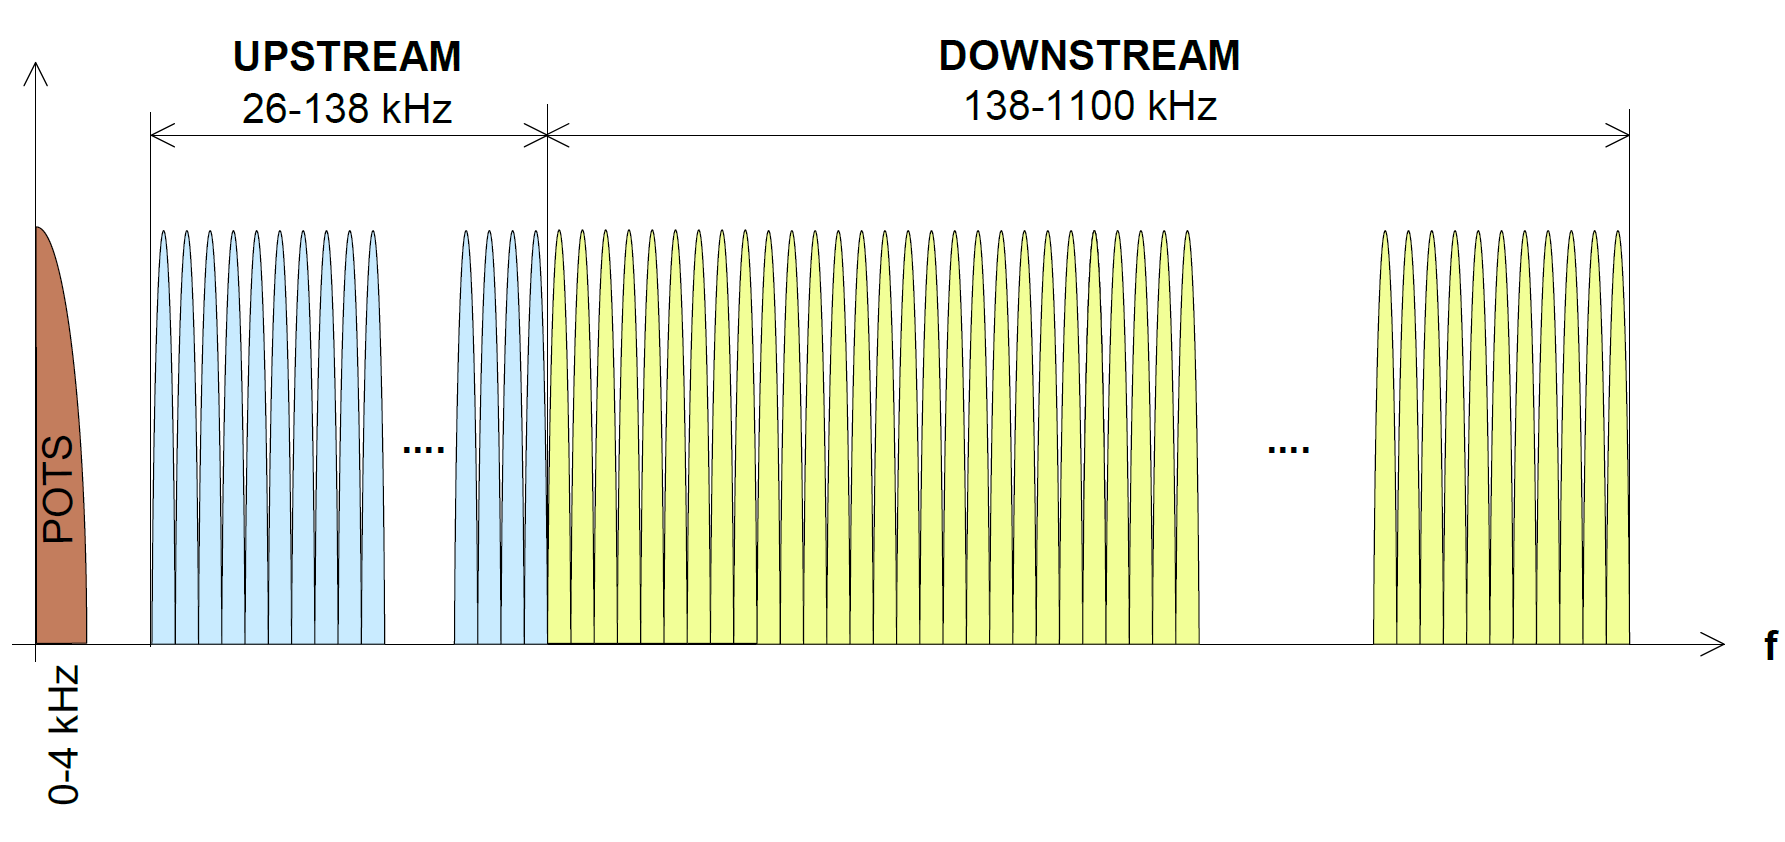
\includegraphics[width=10cm]{obsazeniAdsl.png}
    \caption{Obsazení spektra systémem ADSL}
    \label{fig:adslObsazeni}
\end{figure}
\begin{figure}[ht]
    \centering
    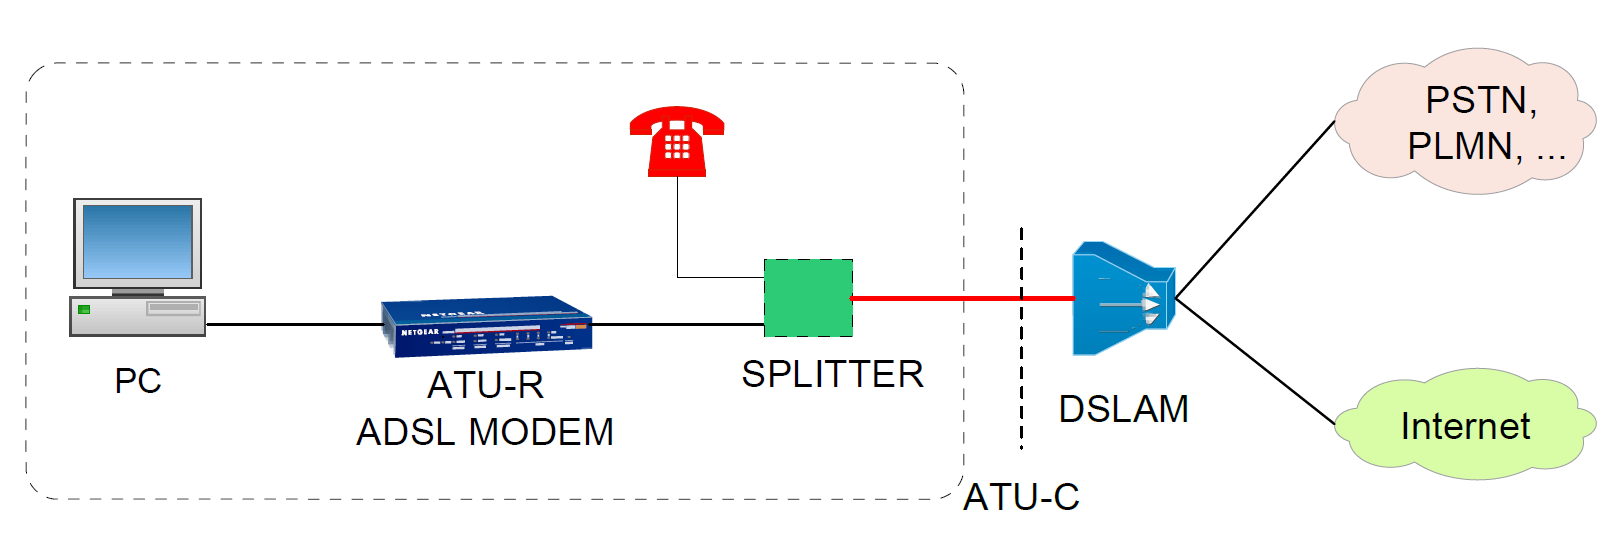
\includegraphics[width=10cm]{architekturaAdsl.png}
    \caption{Architektura systému ADSL}
    \label{fig:architekturaAdsl}
\end{figure}

\paragraph{ADSL2}
\begin{itemize}
\item zavedení rámců flexibilní struktury (délky)
\item 12UP 3,5Down
\end{itemize}

\paragraph{ADSL2+}
\begin{itemize}
\item rozšíření do 2,208 MHz, 511 subnosných
\item až 24Mbit/s DOWN
\end{itemize}

\paragraph{VDSL}
\begin{itemize}
\item nelze použít EC, užití FDD
\item rozšíření až k 8,5MHz za cenu snížení dosahu někam k 1,6km
\item 52Mbit/s DOWN, 6,4Mbit/s UP
\end{itemize}

\paragraph{VDSL+}
\begin{itemize}
\item zdvojnásobení rozteče na 8,6KHz
\item Šírka pásma až 30MHz
\item teoreticky až 100Mbit/s
\end{itemize}

\subsubsection{DOCSIS}
\begin{itemize}
\item Využití sítí kabelové televize (COAX nebo hybrid fiber coax) pro obousměrný datový přenos
\item CMTS = jádro technologie u poskytovatele $\Rightarrow$ modulace signálu a řízení spojení
\item CM = Cable modem - modem na straně zákazníka
\item tato technologie je nadefinovaná na prvních dvou vrstvách OSI RM
\item na straně poskytovatele nutná optimalizace televizních programů (přeskupení) a uvolnění potřebného pásma pro DOCSIS
\end{itemize}


\begin{figure}[ht]
    \centering
    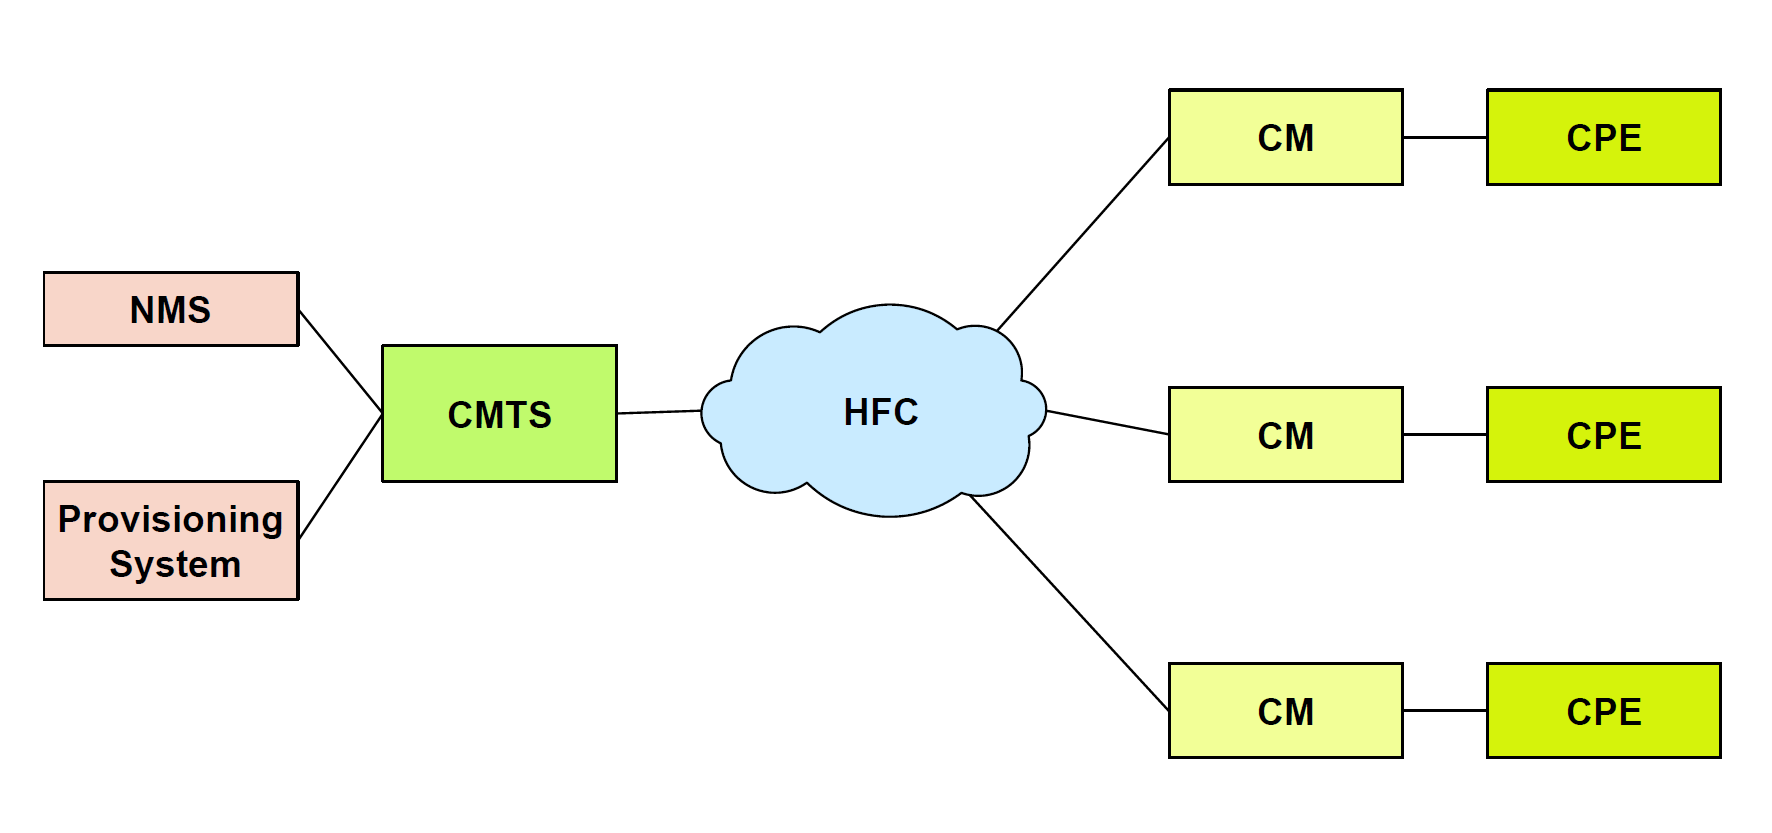
\includegraphics[width=10cm]{architekturaDocsis.png}
    \caption{Architektura systému DOCSIS}
    \label{fig:architekturaDocsis}
\end{figure}

\subsubsection{PON}
\begin{itemize}
\item Pasivní optické sítě
\item OLT - rozhraní mezi poskytovatelem a přístupovou sítí
\item ODN - Distribution network - optická síť přenášející data, patří zde také pasivní rozbočovač, který signály "kopíruje" až do 128 nových toků
\item ONU - na straně zákazníka zakončuje optickou síť a dále pokračuje metalické vedení
\item FTTx
\begin{itemize}
\item FTTC - Curb - Rozvodná skříň od které už vedou metalické kabely do jednotlivých budov
\item FTTB - Building - rozvodná skříň na úrovni budovy - metalické kabely v budově do bytů
\item FTTO - Office -
\item FTTH - Home
\end{itemize}
\item GPON - používá vlastní rámce
\item EPON - používá Ethernet rámce
\end{itemize}

\subsection{Bezdrátové přístupové sítě (Wi-Fi, WIMAX, Bluetooth, Zigbee)}
\subsubsection{Wi-Fi}

\begin{itemize}
\item Standard 802.11; definice dvou spodních vrstev OSI
\item Využití daného pásma metodou Spread Spectrum
\begin{itemize}
\item FHSS(frequency hopping) - pseudonáhodné skoky ve frekvencích, odolné vůči rušení
\item DSSS(direct sequence) - pseudonáhodná maska(kód) známý vysílačem i přijímačem rozprostře každý bit
\item OFDM(orthogonal fr. division multiplexing) - sériový tok převedený na více pomalejších paralelních toků + FDM. Frekvence jsou více zhuštěné, jelikož jsou navzájem ortogonální a neruší se.
\end{itemize}
\end{itemize}
\begin{figure}[ht]
    \centering
    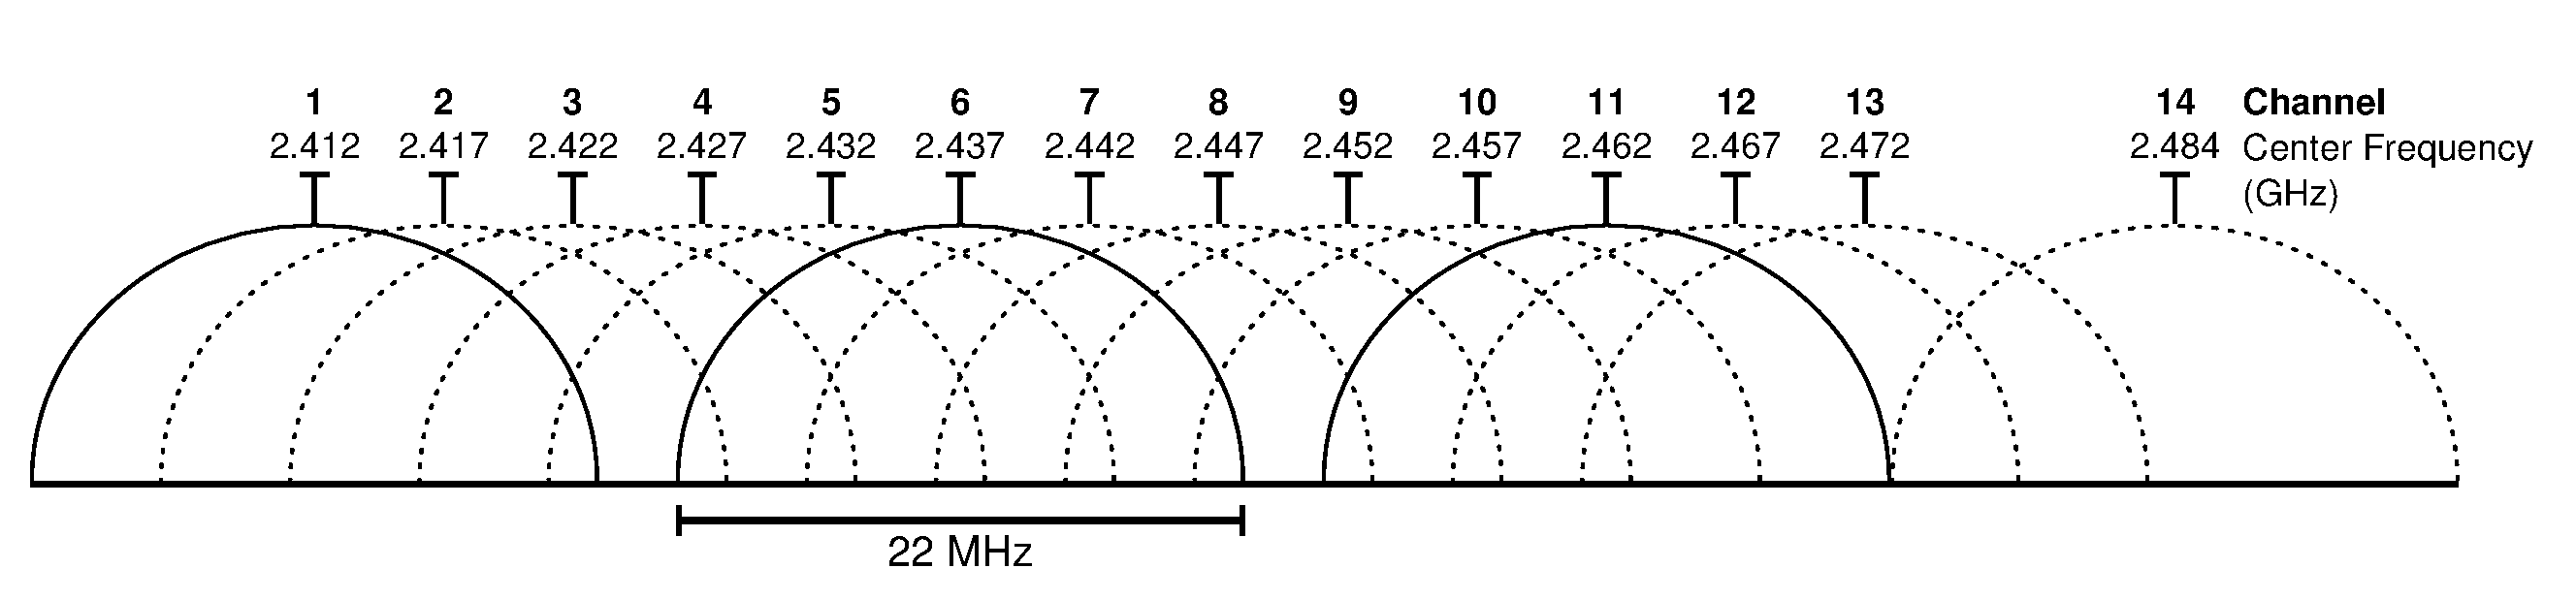
\includegraphics[width=10cm]{wifiChannels.pdf}
    \caption{Kanály Wi-Fi}
    \label{fig:Wi-FiChannels}
\end{figure}
\subsubsection{WIMAX}
\begin{itemize}
\item Standard 802.16; definice dvou spodních vrstev OSI
\item Jde o standard pro bezdrátovou distribuci dat zaměřený na venkovní sítě, tedy jako doplněk k Wi-Fi chápanému jako standard pro vnitřní sítě.
\item Používá OFDM
\end{itemize}

\subsubsection{Bluetooth}
\begin{itemize}
\item pracuje spolu s některými Wi-Fi zařízeními na kanálu 2,4Ghz
\item k přeskokům používá FHSS
\item řazení dle výkonu na 3 třídy(1 - 100mW,2 - 2.5mW a 1mW s resp. dosahem ~100, 10 a 1 metr)
\item řazení dle standardu na BT1.2, 2.0, 3.0 a dnes 4.0
\item na rozdíl od Wi-Fi a ostatních je nadefinován na všech 7 vrstvách OSI RM
\end{itemize}

Topologie
Bluetooth podporuje jak dvoubodovou, tak mnohabodovou komunikaci. Pokud je více stanic propojeno do ad-hoc sítě (tzv.piconet), působí jedna rádiová stanice jako řídící (master) a může simultánně obsloužit až 7 podřízených (slave) zařízení. Všechna zařízení v pikosíti se synchronizují s taktem řídící stanice a se způsobem přeskakování mezi kmitočty. Specifikace dovoluje simultánně použít až 10 pikosítí na ploše o průměru 10 metrů a tyto pikosítě dále sdružovat do tzv. „scatternets“ neboli „rozprostřených“ sítí.
\subsubsection{Zigbee}
\begin{itemize}
\item 802.15.4
\item Podobné Bluetooth, není však kladen důraz na rychlost a objem dat, ale na spolehlivost a lehkou implementaci
\item Uplatnění - PC periferie, automatizace budov, dálkové ovládání, průmyslová automatizace
\end{itemize}

\subsection{Mobilní rádiové sítě (1. až 4. generace)}
\subsubsection{1. Generace}

\begin{itemize}
\item čistě analogové přístroje užívající FDMA
\item zástupci jsou NMT (Nordic Mobile Telephony) a AMPS (Advanced Mobile Phone System)
\item hodně standardů, hodně zájemců a malé kapacitní možnosti $\Rightarrow$ rozšíření na 2G
\end{itemize}
\subsubsection{2. Generace}

\begin{itemize}
\item \textbf{GSM} v Evropě a \textbf{CDMA One} v Americe
\item Neuzavřený systém - přístup i do jiných sítí
\item 3 hlavní složky
\begin{itemize}
\item BSS - Subsystém základnových stanic - poskytuje a spravuje přenosové cesty mezi mobilními stanicemi a NSS
\item NSS - Síťový a spínací subsystém - hlavní část sítě, napodobuje funkce klasické telefonní ústředny
\item OSS - Operační podpůrný subsystém - administrativní fce používané zaměstnanci operátora
\end{itemize}
\item Změna přístupu na kombinaci TDMA a FDMA
\item přechod z analogových zařízení na digitální
\item nové služby jako zprávy a email
\item zmenšení buněk $\rightarrow$ snížení vysílacího výkonu, lepší odolnost a zvýšení bezpečnosti
\item existují dva mezistupně označované jako 2.5G a 2.75G,resp. GPRS a EDGE = připojení k internetu a později zvýšení rychlosti internetu užitím 8-PSK
\end{itemize}

\begin{figure}[ht]
    \centering
    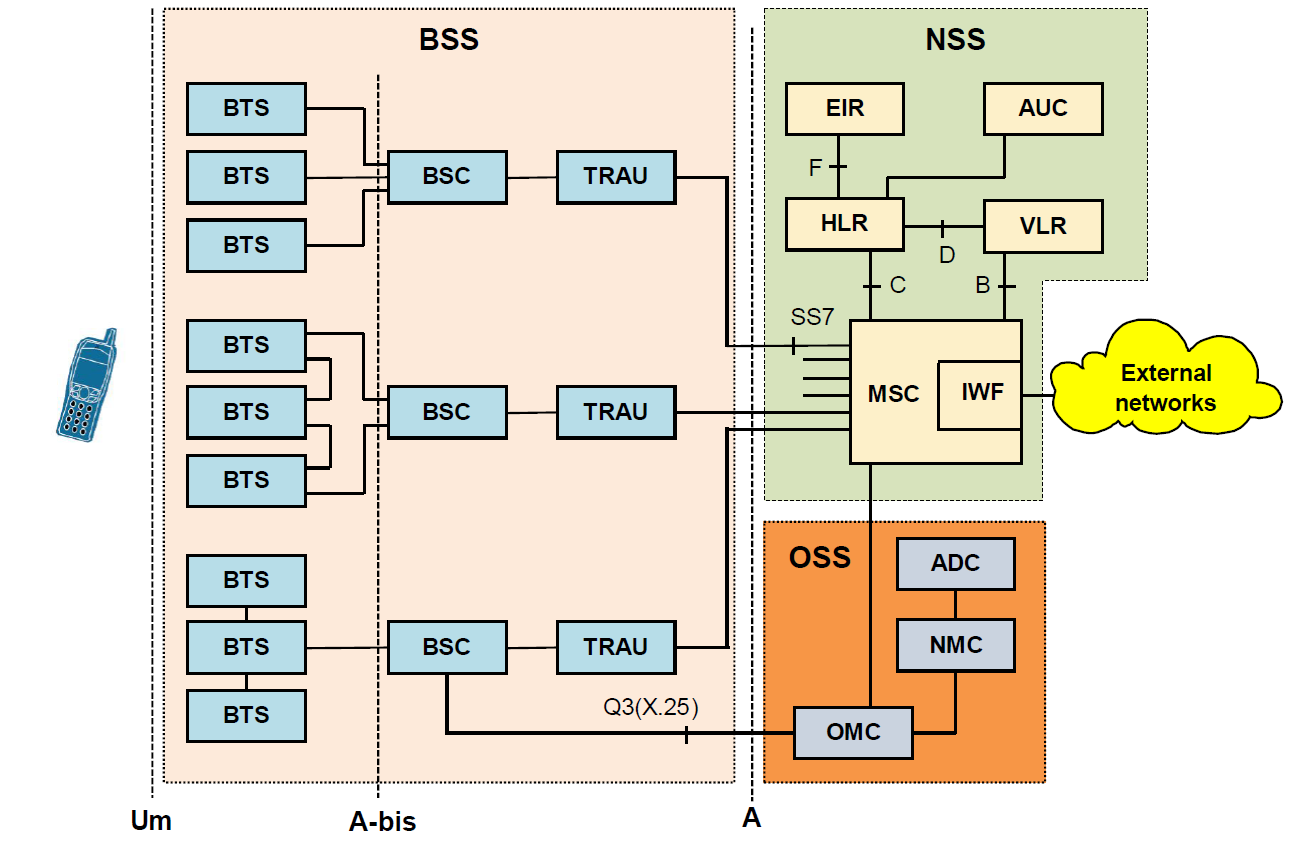
\includegraphics[width=10cm]{gsmArchitektura.png}
    \caption{Architektura systému GSM}
    \label{fig:gsmArchitektura}
\end{figure}

\subsubsection{3. Generace}

\begin{itemize}
\item = UMTS
\item Hlavním rozdílem je, že namísto rádiové přístupové sítě GSM RAN/GERAN se nyní užívá tzv. UTRAN
\item Orientovány na širokopásmový přenos dat
\item Plně digitální, značné navýšení rychlosti přenosu dat
\item CDMA metoda přístupu, resp. WCDMA, což je CDMA s rozprostíráním
\item Architektura ze 3 hlavních prvků
\begin{itemize}
\item UE - user equipment = SIM karta
\item UTRAN - rádiová přístupná část
\item CN - Core network = jádro (mobilní ústředna + databáze a registry)
\end{itemize}
\end{itemize}
\begin{figure}[ht]
    \centering
    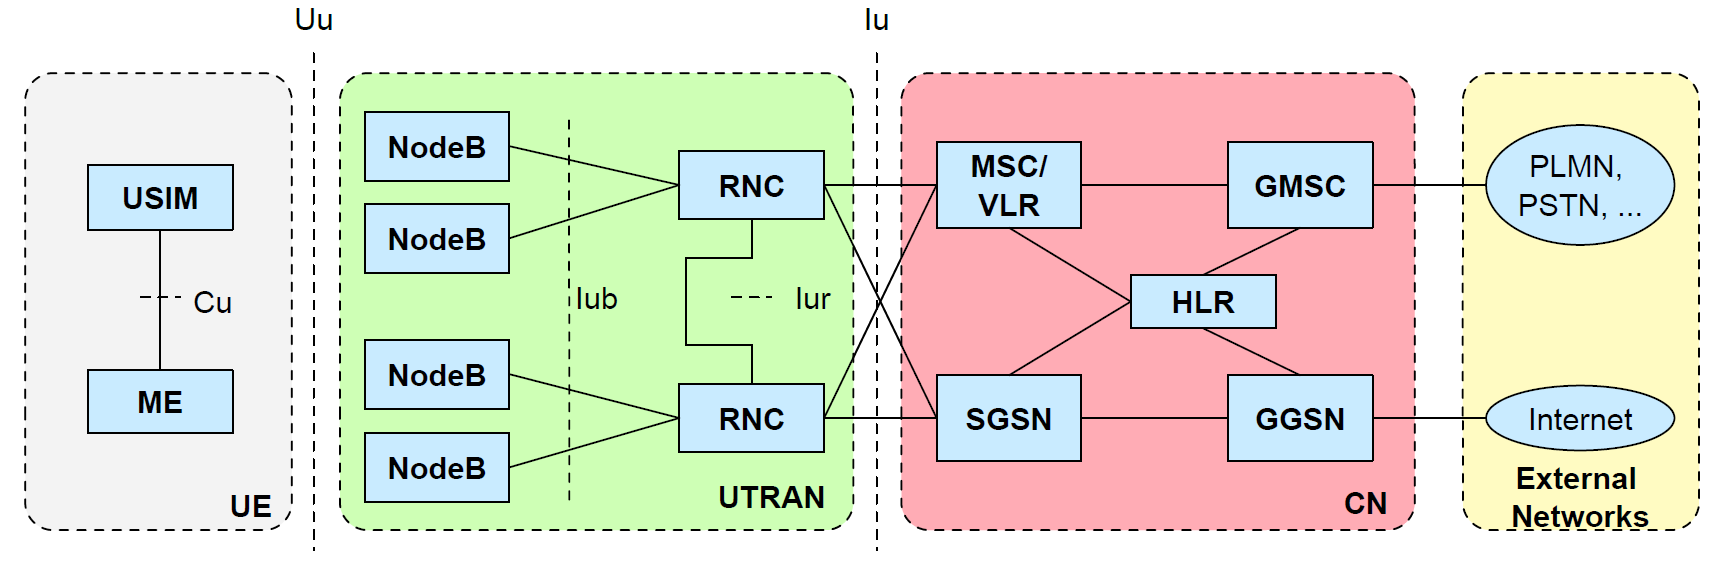
\includegraphics[width=10cm]{umtsArchitektura.png}
    \caption{Architektura systému UMTS}
    \label{fig:umtsArchitektura}
\end{figure}
\subsubsection{4. Generace}

\begin{itemize}
\item LTE = long term evolution
\item formálně LTE ještě patří do 3 a do 4G patří až LTE Advanced
\item Celá síť je datově orientovaná, hlas je rovněž reprezentován jako data a ne jako zvuk.
\item OFDM namísto WCDMA
\end{itemize}

\newpage
\section{Úvod do teoretické informatiky}

\subsection{Množiny, relace, funkce}
\subsubsection{Množina}
\begin{itemize}
\item Souhrn předmětů (prvků) chápaných jako celek/ Kolekce vzájemně odlišitelných objektů - prvků.
\item Definice výčtem x charakteristickou vlastností - M = ${1,2,3}$, $M = {x\in R; x<4}$
\item Na pořadí nezáleží, duplicity nejsou možné ${1,2,2}={2,1}$,${1,2}={2,1}$
\item Velikost = $|X|$; $X = {1,2,2}$; $|X| = 2$
\begin{itemize}
\item Nekonečná x Konečná
\item Prázdná množina = $\varnothing ,|\varnothing | = 0 != {\varnothing }, |{\varnothing }| = 1$
\end{itemize}
\item Prvek $x$ náležící do množiny M značíme $x \in M$, čteme prvek x náleží do množiny M
\item Podmnožina P množiny M = všechny prvky množiny P jsou obsaženy v množině M (značíme $\subseteq$ )
\begin{itemize}
\item $\forall  A: \varnothing  \subseteq  A$
\item $M\subseteq M$
\item $P={1}, M={1,2} \rightarrow P\subseteq M$
\end{itemize}
\item Operace na množinách
\begin{itemize}
\item \textbf{Průnik} $\rightarrow$ $M \cap N$ = bude obsahovat prvky, které se vyskytují v M i v N
\item \textbf{Sjednocení} $\rightarrow$ $M \cup N$ = bude obsahovat prvky, které se vyskytují v M nebo v N (tzn. i ty co jsou v obou)
\item \textbf{Rozdíl} $\rightarrow$ $M - N$ = bude obsahovat prvky, které jsou v M, ale nejsou v N
\item \textbf{Doplněk} $\rightarrow$ $M'$ = všechny prvky z universa, které M neobsahuje
\item \textbf{Kartézský součin } $\rightarrow$ $M \times N$ = bude obsahovat uspořádané dvojice - první člen z M druhý z N
\item \textbf{Potenční množina $2^M$} -
\end{itemize}
\end{itemize}

\subsubsection{Relace}

\begin{itemize}
\item Libovolný vztah mezi skupinou prvků jedné nebo více množin
\item Klasifikace dle arity - unární, binární, ternární,... n-ární - množina uspořádaných n-tic
\item Binární relace = množina uspořádaných dvojic, např. R = {(a,a),(b,b),(c,c)}
\item U binární relace je možno definovat vlastnosti jako je reflexivita, symetrie, antisymetrie, tranzitivita
\item Zobrazení z množiny X do množiny Y je relace R $\subseteq  X \times Y $, kde platí, že pro každý prvek $x \in X$ existuje právě jeden prvek $y \in Y$ tak že $(x, y) \in R$.
\end{itemize}
\paragraph{Binární relace}
\begin{itemize}
\item \textbf{Reflexivita} = každý prvek z množiny je v relaci sám se sebou
\begin{itemize}
\item Příkladem reflexivní relace je identita, relace "být menší nebo rovno", relace dělitelnosti, atd.
\end{itemize}
\item \textbf{Ireflexivita} = žádný prvek z množiny není v relaci sám se sebou
\begin{itemize}
\item Příkladem ireflexivní relace je relace "být menší než"
\end{itemize}
\item \textbf{Symetrie} = pokud je prvek a v relaci s b, pak je b v relaci s a; (a,b) $\rightarrow$ (b,a)
\begin{itemize}
\item Příkladem symetrické relace je identita, nerovnost nebo vlastnost typu "mít stejné znaménko"
\end{itemize}
\item \textbf{Antisymetrie} = pokud je (a,b) i (b,a) pak musí platit, že a = b
\begin{itemize}
\item Příkladem antisymetrické relace je relace "být menší nebo rovno".
\end{itemize}
\item \textbf{Asymetrie} = silná antisymetrie = pokud je prvek a v relaci s b, pak b v relaci s a není; (a,b) $\rightarrow$ !(b,a)
\begin{itemize}
\item Příkladem asymetrické relace jsou relace "nerovno", "být menší než" nebo "být větší než".
\end{itemize}
\item \textbf{Tranzitivita} = pokud existuje (a,b) a (b,c) pak existuje i (a,c)
\begin{itemize}
\item Příkladem tranzitivní relace je opět relace "být menší nebo rovno", identita, či relace "být příbuzný" na množině lidí.
\end{itemize}
\item \textbf{Úplnost} - Pro každou dvojici platí, že existuje buď (a,b) nebo (b,a) (nebo i obojí)
\begin{itemize} 
\item Příkladem úplné relace je například relace $\leq$ na libovolné číselné  množině.
\end{itemize}
\end{itemize}

\subsubsection{Funkce}
\begin{itemize}
\item Funkce je název pro zobrazení z nějaké množiny M do množiny čísel (většinou reálných nebo komplexních), nebo do vektorového prostoru
\item Alt.: Funkce na množině $M \subset  R$ je předpis, který každému číslu z množiny D přiřazuje právě jedno R.
\item Množinu M nazvýváme Definičním oborem funkce a R nazýváme Oborem hodnot funkce.
\item U funkcí můžeme rozhodovat o mnohých vlastnostech (spíše záležitost matematiky ale co)
\begin{itemize}
\item Monotónnost funkce - určuje zda funkce v daném intervalu klesá či stoupá
\item Sudá funkce - symetrická podle osy Y $\rightarrow$ f(x) = -f(x)
\item Lichá funkce - symetrická podle osy X a Y $\rightarrow$ -f(x) = f(-x)
\item Prostá funkce - hodnoty pro různá x z definičního oboru se vždy liší; funkce v celém definičním oboru je stále rostoucí, nebo stále klesající
\item omezenost
\item lokální/globální minima/maxima
\end{itemize}
\end{itemize}

\subsection{Výroková logika, predikátová logika 1. řádu}
\subsubsection{Výroková logika}
\begin{itemize}
\item \textbf{Výrok} - "Jana zmokla" = atomický výrok $\rightarrow$ nedá se rozložit
\item \textbf{Složený výrok} - "Jestliže pršelo, Jana zmokla" - rozložitelný na atomické výroky "Pršelo" a "Jana zmokla"
\item \textbf{Logické spojky} - spojují atomické výroky do složených = $\lnot ,\wedge ,\vee ,\rightarrow,\leftrightarrow$
\item \textbf{Formule} = atomické nebo složené výroky; Pravdivost formulí - vyhodnocují se binárně $(0 \times 1) (T \times F)$
\item Pravdivostní ohodnocení
\begin{itemize}
\item \textbf{Tautologie} - pravdivá ve všech ohodnoceních
\item \textbf{Splnitelná} - existuje alespoň jedno pravdivé vyhodnocení
\item \textbf{Kontradikce} - neexistuje ani jedno pravdivé vyhodnocení ( = není splnitelná)
\item \textbf{Ekvivalence} = dvě formule jsou ekvivalentní, jestliže mají při stejném ohodnocení "v" stejnou pravdivostní hodnotu
\end{itemize}
\item Logické vyplývání - pokud jsou pravdivé předpoklady, pak i závěr je pravdivý - ověření pomocí rezoluční metody
\end{itemize}
Normálové formy - specifický tvar formule, který je ekvivalentní k původnímu
\begin{itemize}
\item DNF - Disjunktivní normálová forma - elementární konjunkce spojené disjunkcemi, př. $(p\wedge q)\vee (\lnot p\wedge r)\vee (p)$
\item CNF/KNF - Konjunktivní normálová forma - elementární disjunkce spojené konjunkcemi, př. $(p\vee \lnot q)\wedge (\lnot p\vee r)\wedge (p)$
\item Úplná K/D normálová forma - v každé části (konjunktu/disjunktu) se vyskytují všechny literály právě jednou, př. $(p\vee q\vee r)\wedge (\lnot p\vee \lnot q\vee r)$ = UKNF
\end{itemize}

\subsubsection{Predikátová logika}
\begin{itemize}
\item Zavedení proměnných
\item \textbf{Universum} - Množina prvků ze kterých můžeme vybírat do proměnných
\item \textbf{Valuace} - přiřazení prvků universa proměnným
\item \textbf{Predikáty} - vrací pravda/nepravda
\begin{itemize}
\item Arita - nulární, unární - n-ární, popisují vlastnosti, či vztahy 0 - n proměnných
\end{itemize}
\item Kvantifikátory - $\forall x$ = pro všechny x platí, $\exists x$ = existuje alespoň jedno x, nelze je aplikovat na konstanty
\item Formule predikátové logiky
\begin{itemize}
\item Atomické formule - mohou obsahovat konstanty (nulární fce), funkce, predikáty a rovnosti
\item Jinak mohou obsahovat kvantifikátory, logické spojky
\end{itemize}
\item \textbf{Termy} - výrazy složené z proměnných, konstant a funkcí reprezentující prvky universa
\item pomocné symboly = "(" + ")"
\end{itemize}

\subsection{Regulární jazyky, konečné automaty}
\subsubsection{Regulární jazyky}
\begin{itemize}
\item Nejjednodušší formální jazyk. Formální jazyk je množina slov nad nějakou abecedou.
\item \textbf{Abeceda} = neprázdná konečná množina symbolů/znaků
\item \textbf{Slovo} = konečná posloupnost znaků z konkrétní abecedy
\item \textbf{Jazyk} = množina (některých) slov tvořených symboly z dané abecedy
\item \textbf{Délka slova} = počet symbolů, \textbf{prázdné slovo} = slovo o délce 0
\item Zřetězení slov = $OST \cdot RAVA$ = $OSTRAVA$
\item Operace na jazycích = sjednocení, průnik, doplněk, rozdíl, zřetězení, iterace
\item Iterace jazyka = zřetězení libovolného počtu (0-n) slov z jazyka
\item \textbf{Regulární jazyk} = prázdný jazyk + jazyk obsahující právě jeden znak z abecedy + jazyky vzniklé operacemi popsanými výše nad těmito jazyky
\item Zrcadlový obraz slova $w = w^R$ je slovo $w$ zapsané "pozpátku" AHOJ $\rightarrow$ JOHA
\end{itemize}

\subsubsection{Konečné automaty}
\begin{itemize}
\item Výpočetní model generující formální jazyky
\item Popisuje velice jednoduchý počítač, který může být v jednom z několika stavů, mezi kterými přechází na základě symbolů, které čte ze vstupu
\item Konečný automat = deterministický = vždy je jasný počáteční stav, vždy je jasné do jakého stavu se přejde při daném vstupu, vždy jsou jasné přijímací stavy.
\item Formálně je konečný automat definován jako uspořádaná pětice ($Q, \Sigma, \delta, q_0, F$) (názvy se mohou lišit)
\begin{itemize}
\item $Q$ = neprázdná množina stavů
\item $\Sigma$ = neprázdná množina vstupních symbolů (abeceda)
\item $\delta$ = pravidla přechodů mezi stavy (pro každý stav, n pravidel (n=počet symbolů v abecedě))
\item $q_0$ = počáteční stav (právě jeden)
\item $F$ = množina přijímacích stavů
\end{itemize}
\end{itemize}

% http://madebyevan.com/fsm/
\begin{center}
\begin{tikzpicture}[scale=0.2]
\tikzstyle{every node}+=[inner sep=0pt]
\draw [black] (19.6,-19.8) circle (3);
\draw (19.6,-19.8) node {$1$};
\draw [black] (19.6,-19.8) circle (2.4);
\draw [black] (35.5,-19.8) circle (3);
\draw (35.5,-19.8) node {$2$};
\draw [black] (19.6,-35.2) circle (3);
\draw (19.6,-35.2) node {$3$};
\draw [black] (35.5,-35.2) circle (3);
\draw (35.5,-35.2) node {$4$};
\draw [black] (35.5,-35.2) circle (2.4);
\draw [black] (48.8,-26.5) circle (3);
\draw (48.8,-26.5) node {$5$};
\draw [black] (48.8,-26.5) circle (2.4);
\draw [black] (22.6,-19.8) -- (32.5,-19.8);
\fill [black] (32.5,-19.8) -- (31.7,-19.3) -- (31.7,-20.3);
\draw (27.55,-20.3) node [below] {$a$};
\draw [black] (38.18,-21.15) -- (46.12,-25.15);
\fill [black] (46.12,-25.15) -- (45.63,-24.34) -- (45.18,-25.24);
\draw (41.16,-23.65) node [below] {$b$};
\draw [black] (51.714,-25.838) arc (130.53597:-157.46403:2.25);
\draw (56.12,-28.5) node [right] {$b$};
\fill [black] (51.1,-28.41) -- (51.24,-29.34) -- (52,-28.69);
\draw [black] (17.219,-17.995) arc (260.56505:-27.43495:2.25);
\draw (15.59,-13.26) node [above] {$b$};
\fill [black] (19.58,-16.81) -- (20.21,-16.1) -- (19.22,-15.94);
\draw [black] (19.6,-32.2) -- (19.6,-22.8);
\fill [black] (19.6,-22.8) -- (19.1,-23.6) -- (20.1,-23.6);
\draw (20.1,-27.5) node [right] {$a$};
\draw [black] (33.35,-33.11) -- (21.75,-21.89);
\fill [black] (21.75,-21.89) -- (21.98,-22.8) -- (22.68,-22.08);
\draw (28.51,-27.02) node [above] {$a$};
\draw [black] (35.5,-22.8) -- (35.5,-32.2);
\fill [black] (35.5,-32.2) -- (36,-31.4) -- (35,-31.4);
\draw (36,-27.5) node [right] {$a$};
\draw [black] (46.29,-28.14) -- (38.01,-33.56);
\fill [black] (38.01,-33.56) -- (38.95,-33.54) -- (38.41,-32.7);
\draw (41.21,-30.35) node [above] {$a$};
\draw [black] (32.5,-35.2) -- (22.6,-35.2);
\fill [black] (22.6,-35.2) -- (23.4,-35.7) -- (23.4,-34.7);
\draw (27.55,-34.7) node [above] {$b$};
\draw [black] (22.6,-35.2) -- (32.5,-35.2);
\fill [black] (32.5,-35.2) -- (31.7,-34.7) -- (31.7,-35.7);
\draw [black] (12.2,-19.8) -- (16.6,-19.8);
\fill [black] (16.6,-19.8) -- (15.8,-19.3) -- (15.8,-20.3);
\end{tikzpicture}
\end{center}

\subsection{Algoritmy a algoritmické problémy, výpočetní modely}
\subsubsection{Algoritmus}
Zpracovává vstup a generuje výstup
\begin{itemize}
\item Řídící tok - sekvence vykonávání jednotlivých kroků, včetně větvení a cyklů
\item Dva typy instrukcí - instrukce pracující s daty, instrukce ovlivňující řídící tok(větvení, cykly, návraty,...)
\item Algoritmus je vykonáván strojem - např. reálný stroj, virtuální stroj, matematický model
\item Stroj pracuje po krocích, v každém kroku se nějak změní konfigurace = popis celkového stroje(paměť, stav)
\item Výpočet algoritmu - začíná se v počáteční konfiguraci, každý krok přejde do jiné konfigurace, výpočet končí v koncové konfiguraci
\item Invarianta - podmínka, která musí být splněna vždy, na konkrétním místě v algoritmu
\item např invarianta pro cyklus $i=0;while(i<10)\{i++\}$ je, že $0 >= i <= 10$. Jelikož posledním krokem v cyklu bude, že se $i$ nastaví na 10 a kdykoliv to je mimo, to do cyklu vůbec nespadne.
\item pro každý řídící stav (vrchol grafu řídícího toku) lze určit invariantu
\item Korektnost - Žádná nepovolená operace, výpočet je konečný, výstup odpovídá zadání.
\end{itemize}
\subsubsection{Výpočetní modely}

\begin{itemize}
\item idealizované modely počítače používané pro výpočet složitosti
\item Definují množinu povolených operací
\item Turingův stroj
\begin{itemize}
\item Church-Turingova teze = ke každému algoritmu existuje Turingův stroj
\item Respektive pokud nelze problém popsat Turingovým strojem, není tento problém algoritmicky rozhodnutelný
\item Formálně je Turingův stroj šestice
\begin{itemize}
\item Množina vnitřních stavů
\item Konečná abeceda symbolů na pásce
\item Konečná množina vstupních symbolů (podmnožina abecedy)
\item počáteční stav
\item Přechodová funkce vpravo, či vlevo
\item Množina koncových stavů
\end{itemize}
\end{itemize}
\item RAM stroj
\begin{itemize}
\item Z hlediska výpočetní síly ekvivalentní Turingovu stroji
\end{itemize}
\item Lambda kalkulus
\item Konečný automat
\end{itemize}

\subsection{Algoritmicky nerozhodnutelné problémy}
Pro rozhodovací problém P neexistuje žádný algoritmus. Tato problematika je zkoumána vědním oborem - Teorií vyčíslitelnosti. Každý algoritmus který je rozhodnutelný, lze zároveň přeložit do jazyka Turingova stroje.
Příkladem takových to problémů je např. Problém zastavení
\subsection{Výpočetní složitost algoritmů, asymptotická notace}\label{sec:uti_slozitost}
\begin{itemize}
\item U algoritmů řešíme zpravidla dva typy složitosti
\begin{itemize}
\item \textbf{Časovou složitost} - jak závisí doba výpočtu na množství vstupních dat
\item \textbf{Paměťovou náročnost} - jak závisí množství použité paměti na množství vstupních dat
\end{itemize}
\item \textbf{Velikost vstupu} - hodnota udávající velikost vstupu - počet prvků v sekvenci, počet znaků v řetězci, atp.
\item přesnou dobu výpočtu můžeme uvádět jako počet kroků nebo počet sekund
\item Zpravidla se zaobíráme nejhorším případem, někdy je však vhodné se zaobírat i průměrným případem
\item U funkce vyjadřující časovou složitost nám většinou stačí odhad - zanedbáme méně významné členy $a\cdot n^2+b \Rightarrow n^2$
\end{itemize}
\subsubsection{Asymptotická notace}
\begin{itemize}
\item Popisují jak rychle daná funkce roste
\item $O(f)$ - množina všech funkcí, které rostou nejvýše tak rychle jako f
\item $\Omega(f)$ – množina všech funkcí, které rostou alespoň tak rychle jako f
\item $\Theta(f)$ – množina všech funkcí, které rostou stejně rychle jako f
\end{itemize}
\newpage
\section{Architektury počítačů, Počítačové sítě}
\subsection{Protokolová rodina TCP/IP a její vztah k referenčnímu modelu ISO‐OSI. Překlad síťových adres - NAT, IPv6 - specifika nové verze protokolu}
\subsubsection{TCP/IP a její vztah k referenčnímu modelu ISO‐OSI}
\begin{table}[ht]
\centering
\begin{tabular}{|c|c|c|}
\hline
                           & TCP/IP                                             & RM OSI      \\
\hline
\multirow{5}{*}{Protokoly} & \multirow{3}{*}{Aplikační(HTTP, FTP, SMTP... )}    & Aplikační   \\
                           &                                                    & Prezentační \\
                           &                                                    & Relační     \\
                           & Transportní (TCP, UDP)                             & Transportní \\
                           & Síťová (IP)                                        & Síťová      \\
\hline
\multirow{2}{*}{Networks}  & \multirow{2}{*}{Síťové rozhraní (LAN, ARPANET...)} & Linková     \\
                           &                                                    & Fyzická    \\
\hline
\end{tabular}
\caption{TCP/IP vs RM OSI}
\label{tab:tcpipvsosi}
\end{table}


\begin{itemize}
\item Na aplikační vrstvě běží nějaký aplikační protokol, FTP, HTTP, SMTP, DNS...
\item Na transportní vrstvě pak buď TCP nebo UDP.
\begin{itemize}
\item TCP přebere od aplikační vrstvy data, rozdělí na segmenty, očísluje a seřadí. Provádí kontrolu a vyžaduje potvrzení o příjetí dat pro případ znovu poslání atp.
\item UDP funguje podobně, ale kašle na kontrolu. Fire-and-forget. Ztráta jednoho packetu je v klidu aka bez jednoho vojáka válka bude. Přenos videa např.
\end{itemize}
\item Síťová vrstva pak k segmentu přidá hlavičku a vytvoří IP datagram. - provádí tedy adresování a směrování.
\end{itemize}

\subsubsection{Překlad síťových adres - NAT}
\begin{itemize}
\item Jedná se o překlad adres z vnitřní sítě na adresy vnější sítě (např. Internetu)
\item Nemusíme mít na nějakou podsíť 1:1 adresy.
\item Nevýhoda je, že to limituje komunikaci s internetem. Nebo když máme asymetrické směrování (vnitřní síť je propojena s vnější sítí přes víc než 1 router).
\item Tyto údaje/překlady si uchovává v NAT tabulce.
\item Static vs Dynamic NAT $\rightarrow$ manuálně překonfigurované nebo využití dynamického poolu.
\end{itemize}

\subsubsection{IPv6 - specifika nové verze protokolu}
\begin{itemize}
\item Hlavní změna je daleko větší adresní prostor. (IPv4 $2^{32}$ vs. IPv6 $2^{128}$).
\item Pro každého ze 7miliard lidí na zemi teoreticky připadá $5*10^{28}$ adres.
\item Je odstraněna potřeba použití NATu, který byla zaveden kvůli vyčerpání adresního prostoru IPv4.
\item Jedná se o 128bitové hexadecimální adresy.
\item FEDC:0A98:7654:1230:0000:0000:7546:3210 - kde leading zeros may be omitted $\rightarrow$ FEDC:A98:7654:1230:::7546:3210
\item SLAAC (Stateless Address Autoconfig) - router má prefix a k němu se přidá MAC adresa zařízení.
\item Některé protokoly už jsou zavedeny jako součást (IPSec), u IPv4 byl volitelný, ale skoro vždy implementovaný.
\item Nezná broadcast, pouze multicast na všechny adresy (...)
\end{itemize}
\begin{figure}[ht]
    \centering
    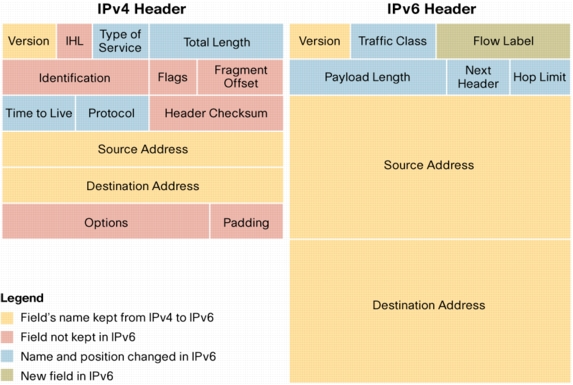
\includegraphics[width=10cm]{ipv6.jpg}
    \caption{Hlavičky protokolů IPv4 a IPv6}
    \label{fig:ipHeaders}
\end{figure}


\subsection{Aktivní prvky počítačových sítí a jejich funkce - rozbočovač, přepínač, směrovač.}
\subsubsection{Rozbočovač - HUB}

\begin{itemize}
\item Nejjednodušší aktivní prvek
\item Chová se jako opakovač - cokoliv přijde na nějaký port je zopakováno pro všechny porty v něm.
\item Původně sloužily opakovače u starých sítí při moc dlouhém koaxu, který při své délce už ztrácel signál, tak se tam jebunl opakovač.
\end{itemize}
\subsubsection{Přepínač - SWITCH}

\begin{itemize}
\item Nahradil hub - už skoro ví, co kam posílat a nekopíruje - posílá to na daný interface/port.
\item Když přijde rámec směrovaný na doposud neznámou adresu (MAC), pošle ho všem a jedna ze stanic se ozve, tím pádem si to doplní do tabulky, na který port/interface to má příště směrovat.
\end{itemize}
\subsubsection{Směrovač - ROUTER}

\begin{itemize}
\item Nejvyspělejší aktivní prvek
\item L3 zařízení $\rightarrow$ má ponětí o IP adresách.
\item Dokáže provádět směrovaní podle algoritmů a tím tak vybírat nejlepší cestu pro paket.
\item Realizuje překlad adres (NAT)
\item Filtrace paketů
\item V dnešní době se často používají L3 switche, které mají stejnou funkcionalitu.
\end{itemize}
\subsection{Služby Internetu a jejich protokoly: elektronická pošta (SMTP, POP, IMAP), WWW, SSH a Telnet. Systém DNS}
\subsubsection{SMTP}
\begin{itemize}
\item Simple Mail Transfer Protocol
\item Slouží pouze k odesílání emailů
\item Využívá TCP nad portem 25
\end{itemize}

\subsubsection{POP3}

\begin{itemize}
\item Slouží pouze pro stahování pošty
\item TCP/110
\item Stáhne email a odpojí se, prohlížení je pak "offline". Moderní POP3 stahují pouze hlavičky a obsah emailu až po rozkliku.
\end{itemize}
\subsubsection{IMAP}

\begin{itemize}
\item Protokol pro vzdálený přístup k emailové schránce.
\item Na rozdíl od POP3 vyžaduje stále připojení.
\item Stahuje pouze hlavičky. Obsah až po rozkliku.
\item Umožňuje více klientů být připojeno na jednu schránku + udržuje informace o stavu emailu (jestli byl přečtený atp.) + synchronizuje to mezi klienty. (Dobré u service desku třeba?)
\end{itemize}
\subsubsection{WWW}

\begin{itemize}
\item World Wide Web - systém pro prohlížení obsahu Internetu
\item Pro komunikaci se využívá komWorld Wide Web - systém pro prohlížení obsahu Internetu
\item Pro komunikaci se využívá komunikační protokol HTTP/HTTPS
\item HTTP slouží pro přenos hypertextových dokumentů (HTML) - TCP/80
\item HTTPS navíc zajišťuje i zabezpečené spojení pomocí SSL - TCP/443
\end{itemize}
\subsubsection{Telnet}
\begin{itemize}
\item Protokol aplikační vrstvy, používá se pro propojení klient-server pod protokolem TCP.
\item Původně emulace terminálu u vzdáleného přístupu.
\item Hlavní nevýhoda je, že přenos není šifrovaný $\rightarrow$ díky tomu vznik SSH
\item Dříve to bylo OK, nebyla potřeba moc bezpečnost, používal se na univerzitních sítích atp, ale dnes v dobách Internetu je to průser.
\end{itemize}

\subsubsection{SSH}
\begin{itemize}
\item Náhrada za telnet
\item Šifruje data
\item TCP/22
\item SFTP (SSH FTP)
\end{itemize}

\subsubsection{DNS}
\begin{itemize}
\item Překlad IP Adres na lépe zapamatovatelná jména
\item Hierarchické rozdělení jmen.
\item Každá noda max 63 charů, celá adresa max 256. Case insensitive, national characters possible, ale nedoporučuje se.
\item Top-Level Domains: generic (.edu, .com, .org, .net) nebo national (.cz, .uk)
\item Primární a Sekundární Name Servery (NS) - data jsou trvale uloženy v primárním, sekundární si je nakopírujou. Když je update u primárního, admin musí zvýšit verzi aby došlo k synchronizaci - tohle je častá chyba. Oba jsou autoritativní.
\item Resolver je část OS na klientově straně, která komunikuje s NS.
\item TCP/UDP
\end{itemize}

\subsection{Bezpečnost počítačových sítí s TCP/IP: útoky, paketové filtry, stavový firewall. Šifrování a autentizace, virtuální privátní sítě}
\begin{itemize}
\item utajení (confidentality) – posluchač na kanále datům nerozumí
\item autentizace (authentication) – jistota, že odesílatel je tím, za koho se vydává
\item integrita (integrity) – jistota, že data nebyla na cestě zmodifikována
\item nepopiratelnost (non-repudiation) – zdroj dat nemůže popřít jejich odeslání
\end{itemize}

\subsubsection{Útoky na počítačové sítě}
denial of service (DoS): Cílem útočníka vyčerpání systémových prostředků (paměť, CPU, šířka pásma)síťového prvku nebo serveru a jeho zhroucení nebo změna požadovaného chování Záplava pakety SYN neboli SYN-flood je druh útoku označovaný jako DoS. Útočník pošle posloupnost paketů s příznakem SYN cílovému počítači, ale již dále neodpovídá. Brute Force
\subsubsection{Packetové filtry}
\paragraph{ACL}

\begin{itemize}
\item nejčastěji na rozhraní směrovačů, filtrace podle informací ze síťové a vyšších vrstev
\item reflexivní ACL - Automaticky propouští vstupní provoz, který odpovídá povolenému provozu výstupním
\end{itemize}
\paragraph{Stavový firewall}

\begin{itemize}
\item je v informatice označení pro takový firewall, který podporuje SPI (anglicky Stateful packet inspection), což znamená, že je schopen sledovat a udržovat všechny navázané TCP/UDP relace (pracuje na transportní vrstvě referenčního modelu ISO/OSI). Stavový firewall je schopen rozlišovat různé stavy paketů v rámci jednotlivých relací (spojení) a jeho úkolem je propustit pouze takové, které patří do již povolené relace (jiné jsou zamítnuty). Stavový firewall poskytuje vyšší efektivitu kontroly jednotlivých paketu, protože pro existující spojení kontroluje jen stavovou tabulku, místo toho, aby kontroloval u každého paketu sadu nadefinovaných složitých pravidel. Stavový firewall nijak nesouvisí s hloubkovou kontrolou paketů. Je schopný udržovat důležité parametry všech spojení v paměti od začátku až do konce. Nejnáročnější kontrola se provádí v době nastavení spojení.
\end{itemize}
\subsubsection{Šifrování a autentizace}

\begin{itemize}
\item Utajit algoritmus, když se prozradí, je implementace k ničemu
\item Zavést klíče parametrizující algoritmus, je-li dost možných klíčů, může být algoritmus známý
\end{itemize}
\subsubsection{Symetrický systém}

\begin{itemize}
\item Sdílený klíč
\item Implementace algoritmů efektivní (rychlost), lze realizovat hardwarově
\item Algoritmy DES, 3DES, AES, …
\item Autentizace v symetrickém systému - Zakódování username klíčem u odesílatele, stejným klíčem dekódování u příjemce + test smysluplnosti jména (např. připojení Hash hodnoty ke jménu a kontrolní výpočet s porovnáním na přijímači)
\end{itemize}
\begin{figure}[ht]
    \centering
    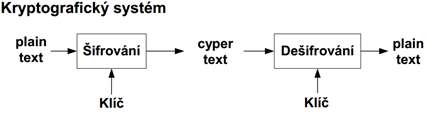
\includegraphics[width=10cm]{sym-sifr.png}
    \caption{Symetrické šifrování}
    \label{fig:symSifr}
\end{figure}
\subsubsection{Asymetrický systém}

\begin{itemize}
\item Klíče se generují jako doplňující se pár – veřejný (public) a soukromý (private) klíč
\item Jeden klíč použit pro šifrování, druhý pro dešifrování (je jedno, který z nich k čemu)
\item Mnohem náročnější na výpočty, pomalejší
\item Asymetrický systém se běžně využívá pro předávání (dynamicky generovaných) klíčů pro symetrický systém.
\end{itemize}
\begin{figure}[ht]
    \centering
    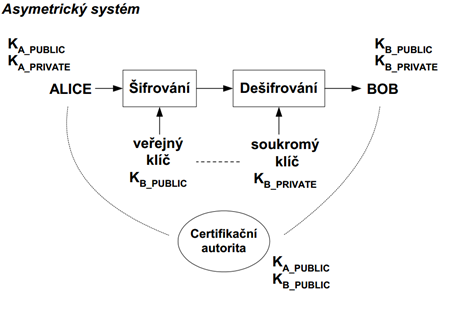
\includegraphics[width=10cm]{asym-sifr.png}
    \caption{Asymetrické šifrování}
    \label{fig:asymSifr}
\end{figure}
\subsubsection{Virtual Private Network (VPN)}
VPN realizuje přenos privátních dat přes veřejnou síť s použitím kryptovacích metod a tunelů Poskytuje autentizaci, integritu dat a utajení. Výhodou cena, flexibilita topologie, odpadá management WAN linek Tunel– virtuální dvoubodové spojení přes veřejnou síť, nese data jednoho protokolu ve druhém protokolu.

\subsection{Architektury počítačů, jejich vlastnosti, principy fungování počítače. Hierarchické uspořádání pamětí v počítači, základní charakteristika jednotlivých pamětí}
\subsubsection{Architektury počítačů, jejich vlastnosti, principy fungování počítače}
\paragraph{Základní principy počítače}
\begin{itemize}
\item Skládá se z: pamětí, řídící jednotky, aritmeticko-logické jednotky (ALU) a vstupní/výstupní jednotky
\item Struktura PC je nezávislá na typu řešené úlohy
\item Následující krok je závislý na předešlém.
\item Instrukce a data jsou v 1 paměti. (Později Harvardská koncepce jinak)
\item Program je tvořen posloupností instrukcí, ty jsou volány tak, jak jsou v paměti
\item Používá se dvojková soustava pro reprezentaci instrukcí, adres, znaků....
\end{itemize}

\paragraph{ Von Neumann vs Harvardská}

\begin{figure}[ht]
    \centering
    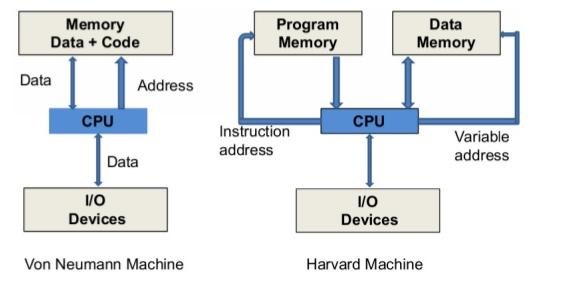
\includegraphics[width=10cm]{app_monolit-arch.png}
    \caption{Von Neumann vs Harvard}
    \label{fig:app_monolit-arch}
\end{figure}
\begin{itemize}
    \item Harvardská koncepce tedy přinesla především rozdělení paměti pro program a pro data $\rightarrow$ program nemůže sám sebe přepsat, můžeme použít odlišné technologie pro tyto dvě paměti, dvě sběrnice = jednoduchý paralelizmus
\end{itemize}
\subsubsection{Hierarchické uspořádání pamětí v počítači, základní charakteristika jednotlivých pamětí}
\paragraph{Podle typu přístupu}
\begin{itemize}
\item RAM - random access memory
\item SAM - serial access memory
\end{itemize}

\paragraph{Podle zápisu/čtení}
\begin{itemize}
\item RWM - read write memory
\item ROM - read only memory
\item WOM - write only memory
\end{itemize}

\paragraph{Podle typu buněk}
\begin{itemize}
\item DRAM - dynamic RAM
\begin{itemize}
\item všechny buňky = kondenzátory. Ten se samovolně vybíjí a je potřeba ho neustále nabíjet (jinak po ~10ms se vybije)
\item informace je tedy uložena ve formě náboje (log 1 / log 0)
\item Buňky jsou uspořádány v matici
\item Prve se čte řádek, pak sloupec.
\item Varianty
\item FP(Fast Page)DRAM, kdy se při dalším čtení už neptá na řádek.
\item S(synchronní)DRAM, která využívá burst mode - zadá se ROW a COL a pak to čte přilehlé
\end{itemize}
\item SRAM - static RAM
\begin{itemize}
\item informace uložena stavem klopného obvodu
\item Méně paměti, ale rychlejší $\rightarrow$ cache paměti, zatímco DRAM pro klasické RAMky
\item paměťové buňky uspořádány do matice
\end{itemize}
\item PROM, EPROM, EEPROM, FLASH - programovatelné paměti.
\begin{itemize}
\item DRAM a SRAM nedrží svůj obsah po odpojení napájení $\rightarrow$ nejsou vhodné pro startovací proces PC $\rightarrow$ proto ROM paměti
\item hlavní náplň těchto pamětí tedy je pamatovat si data i bez napájení
\item Existují nějaké pojistky, když jsou v původním stavu, tak vedou proud (log 0), když je (programátor) přepálí, tak proud nevedou (log 1)
\item Tím pádem po naprogramování do nich (ROM, PROM) už není možný další zápis.
\item EPROM jsou pak paměti, které jdou přeprogramovat, informace se ukládá pomocí elektrického náboje, který je kvalitně izolován. Je ji možné vymazat UV zářením.
\item EEPROM pak jdou vymazat elektrickým impulzem. (Electrically Erasable Programmable ROM)
\item V dnešní době FLASH paměti, což jsou vylepšené EEPROMky, princip stejný.
\end{itemize}
\end{itemize}
\paragraph{L1 a L2 cache}

\begin{itemize}
\item L1
\begin{itemize}
\item Integrována přímo na procesoru
\item Data ze sběrnice (která je pomalá) se ukládají do cache (která je rychlá), a procesor k nim pak přistupuje, když je potřebuje
\end{itemize}
\item L2
\begin{itemize}
\item Mezi mikroprocesorem a pamětí.
\item Data putující mezi těmito dvěma díly uvíznou v cachi, a jestli je bude mikroprocesor znovu potřebovat, tak si pro ně šáhne tam
\item Cache je ovládaná speciálním řadičem, který se snaží predikovat, která data bude mikroprocesor používat.
\end{itemize}
\end{itemize}
\subsection{Základní konstrukční vlastnosti procesorů RISC, principy urychlování činnosti procesorů, predikce skoků. Základní charakteristika a principy činnosti procesorů rodiny Intel od Pentia Pro}
\subsubsection{Základní konstrukční vlastnosti procesorů RISC, principy urychlování činnosti procesorů}

\begin{itemize}
\item Reduced Instruction Set Computer
\item Programátoři/kompilátory většinou využívali jen pár instrukcí - snaha minimalizovat ten instruction set $\Rightarrow$ RISC
\item nejtypičtější vlastnost je tedy malý instrukční soubor.
\item V každém strojovém cyklu by měla být dokončena jedna instrukce. (!= že instrukce trvá jeden cyklus)
\item Instrukce mají pevnou délku a jednotný formát
\item Pro práci s hlavní pamětí se používají výhradně instrukce LOAD a STORE
\item Používá narozdíl od CISC zřetězení instrukcí. Jsou řazeny do fronty. Viz obrázek:
\end{itemize}
\begin{table}[ht]
\centering
\begin{tabular}{l|ll}
\hline
Krok & & Význam               \\
1.& VI & Výběr instrukce      \\
2.& DE & Dekódování instrukce \\
3.& VA & Výpočet adresy       \\
4.& VO & Výběr operandu       \\
5.& PI & Provedení instrukce  \\
6.& UV & Uložení výsledku     \\
\hline
\end{tabular}
\caption{Instrukce}
\label{tab:instrukce}
\end{table}

\begin{table}[ht]
\centering
\begin{tabular}{l|lllllllllllll}
   & T1 & T2 & T3 & T4 & T5 & T6 & T7 & T8 & T9 & T10 & T11 & T12 & T13 \\
   \hline
VI & I1 &    &    &    &    &    & I2 &    &    &     &     &     & ... \\
DE &    & I1 &    &    &    &    &    & I2 &    &     &     &     &     \\
VA &    &    & I1 &    &    &    &    &    & I2 &     &     &     &     \\
VO &    &    &    & I1 &    &    &    &    &    & I2  &     &     &     \\
PI &    &    &    &    & I1 &    &    &    &    &     & I2  &     &     \\
UV &    &    &    &    &    & I1 &    &    &    &     &     & I2  &    
\end{tabular}
\caption{Postup provádění instrukcí procesorem CISC}
\label{tab:instrukceCisc}
\end{table}

\begin{table}[ht]
\centering
\begin{tabular}{l|lllllllllllll}
   & T1 & T2 & T3 & T4 & T5 & T6 & T7 & T8 & T9 & T10 & T11 & T12 & T13 \\ 
   \hline
VI & I1 & I2 & I3 & I4 & I5 & I6 & I7 & I8 & I9 & I10 & I11 & I12 & ... \\
DE &    & I1 & I2 & I3 & I4 & I5 & I6 & I7 & I8 & I9  & I10 & I11 & ... \\
VA &    &    & I1 & I2 & I3 & I4 & I5 & I6 & I7 & I8  & I9  & I10 & ... \\
VO &    &    &    & I1 & I2 & I3 & I4 & I5 & I6 & I7  & I8  & I9  & ... \\
PI &    &    &    &    & I1 & I2 & I3 & I4 & I5 & I6  & I7  & I8  & ... \\
UV &    &    &    &    &    & I1 & I2 & I3 & I4 & I5  & I6  & I7  & ...
\end{tabular}
\caption{Zřetězení provádění instrukcí procesorem RISC}
\label{tab:riscZretezeni}
\end{table}



\paragraph{Problém zřetězení instrukcí} 
\begin{itemize}
\item Datové - např. když instrukce I5 potřebuje v čase T7 hodnotu, kterou I4 uloží až v čase T9.
\item Strukturální - instrukce potřebují pro některé své činnosti sběrnici, která je ovšem k dispozici jen jedné z nich. Přístup je tedy potřeba koordinovat, což přináší zpomalení.
\end{itemize}
\subsubsection{Predikce skoků}

\begin{itemize}
\item Nastává problém, když máme v instrukci podmíněny skok, čili nevíme, jestli se skok provede nebo ne.
\item Nemá smysl zpracovávání pozastavit a čekat na výsledek - lepší je pokračovat ve zpracovávání a pokud se skok neprovede, tak se rozpracovaná fronta instrukcí použije.
\item V opačném případě se rozpracované instrukce ignorují a fronta se začne plnit znovu.
\item K tomu slouží metoda predikce skoku
\item ve formátu instrukcí je vyhrazen jeden bit, predikující zda se skok provede, či nikoliv.
\item Tato predikce může být statická (příslušné bity se vkládají již při kompilaci nebo přímo programátorem) nebo dynamická (predikce se přizpůsobuje aktuálním podmínkám)
\item Dále existuje jednoduchá jednobitová a přesnější dvoubitová predikce skoku, ta je znázorněna následujícím automatem, kde stav A říká, že se provede skok a stav N že neprovede.
\end{itemize}
\begin{figure}[ht]
    \centering
    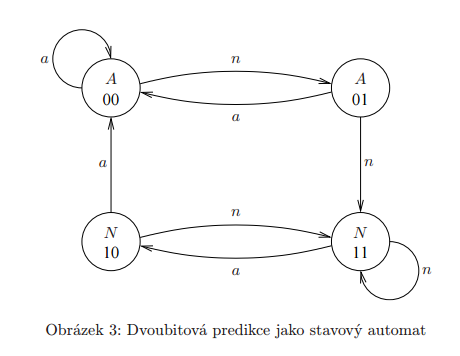
\includegraphics[width=10cm]{predikce.png}
    \caption{Dvoubitová predikce jako stavový automat}
    \label{fig:predikce}
\end{figure}

\subsubsection{Základní charakteristika a principy činnosti procesorů rodiny Intel od Pentia Pro}
\begin{itemize}
\item Pentium PRO přináší zásadní konstrukční změny
\item L2 cache je implementována u procesoru jako samostatný čip se stejnou frekvencí jako procesor
\item Přechod na RISC architekturu, ale bylo potřeba zachovat kompatibilitu s předchozími procesory $\rightarrow$ k tomu slouží Fetch/Decode jednotka, která dekóduje dané instrukce na 118-bitové RISC instrukce
\item Instrukce se ukládají do Instruction Poolu (až 40 mikrooperací)
\item Z tohoto poolu si může jednotka Dispatch/Execute vybírat instrukce mimo pořadí (out-of-order)
\item Provedené instrukce jsou uloženy zpět do banky odkud jsou pomocí jednotky Retire poslána do registrů a L1 cache.
\item Proč je důležite out-of-order? Protože dekodovací jednotka se skládá ze tří menších částí - 2 na jednoduché instrukce a 1 na složitejší, může tak vyprodukovat až 4-mikrooperace v jednom cyklu.
\item Další verze procesorů už představovali pouze modernizace (více tranzistorů, lepší predikce skoků, více cache, atp.)
\end{itemize}
\begin{figure}[ht]
    \centering
    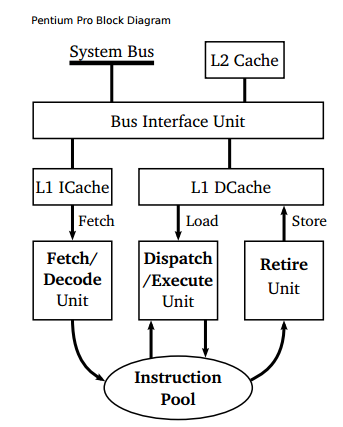
\includegraphics[width=10cm]{ppro.png}
    \caption{Blokové schéma Intel Pentium Pro}
    \label{fig:ppro}
\end{figure}
\newpage
\section{Programování}
\subsection{Principy objektově orientovaného programování (OOP) - třída, objekt, zapouzdření, dědičnost, polymorfismus}

\begin{itemize}
\item \textbf{Třída} - blueprint/vzor, podle kterého pak vytváříme instance. Definujeme vlastnosti a chování.
\item \textbf{Objekt} - jedna instance nějaké třídy.
\item \textbf{Zapouzdření} - veškeré informace, které nejsou potřebné pro klienty modulů, by měly zůstat skryté. (Když chci řídit auto, stačí mi vědět, že musím otáčet volantem a šlapat plyn, nepotřebuji vědět, jak přesně to funguje).
\item \textbf{Dědičnost} - založení nové třídy na základě již existující třídy. Základem je rozšíření původní třídy o nové vlastnosti.
\item \textbf{Polymorfismus} - možnost tříd vystupovat v jiné roli. Např. když mám třídy sjednocené interfacem, můžu pak do nějaké funkce jako parametr dát ten interface a funkci používat se všemi třídami, které ten interface implementují.
\end{itemize}
\subsection{Algoritmy vyhledávání v poli – sekvenční, půlením intervalu, neformální objasnění jejich složitosti}
\subsubsection{Sekvenční}
Nejprimitivnější vyhledávání v poli. Jdeme od prvního prvku až k poslednímu. Klasický for cyklus. Jeho složitost je v nejhorším případě O(n) - buď je na konci nebo není v poli vůbec.
\subsubsection{Půlení intervalu (Binární vyhledávání)}

\begin{itemize}
\item Pole musí být seřazené.
\item Vezmu prvek, který vyhledávám a porovnám ho s prostředním prvkem v poli.
\item Podle toho, jestli je větší nebo menší, tak vyhledávaný prvek musí nutně být v jedné z polovin nebo vůbec.
\item Takhle to pole půlím do té doby, než najdu prvek, který hledám.
\item Jelikož v každém kroku půlím pole a tou špatnou půlkou se vůbec nezabývám, tak se jedná o složitost $log_2(n)$.
\end{itemize}
\subsection{Algoritmy třídění – klasifikace, popis činnosti, neformální objasnění složitosti vybraných algoritmů}
\subsubsection{Klasifikace}
Dvě základní skupiny algoritmů jsou tzv. vnitřní a vnější řazení.
\begin{enumerate}
    \item Vnitřní
    \begin{itemize}
        \item Všechna data uložena v operační paměti a algoritmus k nim může libovolně přistupovat.
    \end{itemize}
    \item Vnější
    \begin{itemize}
        \item Ne všechna data jsou v paměti, nějaká část může být uložena na disku. V případě, že máme moc dat.
    \end{itemize}
\end{enumerate}
Většina třídících algoritmů funguje na principu porovnávání dvou prvků. Některé ale fungují na jiném principu - př. counting sort, který počítá výskyty jednotlivých hodnot. Nebo radix sort.
\subsubsection{Klasifikace algoritmů dle chování}
\paragraph{Řazení výběrem}
\begin{itemize}
\item \textbf{Selection sort}
\begin{itemize}
\item V poli najdeme největší prvek a přesuneme na začátek.
\item Tento prvek "vyřadíme" a hledáme nejvyšší prvek ve zbylém poli.
\item Opakujeme dokud není pole sestupně seřazené.
\item Složitost $n^2$
\end{itemize}
\end{itemize}
\paragraph{Řazení vkládáním}
\begin{itemize}
\item \textbf{Insertion sort}
\begin{itemize}
\item Přesouvá prvky na správné místo.
\item Takhle jdeme postupně od začátku pole až do konce a hledáme, kam ho správně zařadit.
\item Ačkoliv je složitost $n^2$, tak u téměř seřazeného pole se blíží n. U polí s méně než 10 prvky je rychlejší než quick sort.
\end{itemize}
\end{itemize}
\paragraph{Řazení záměnou}
\begin{itemize}
\item \textbf{Bubble sort}
\begin{itemize}
\item Porovnává dva sousední prvky. Pokud je ten vlevo menší, tak je prohodí a postupuje dál. -$\rightarrow$ "probublává na povrch"
\item Vnitřní cyklus se provede $(n-1) + (n-2) + (n-3) +.... = (n^2 - n)/2$ což je složitost $n^2$
\end{itemize}
\item \textbf{Heapsort}
\begin{itemize}
\item Základem je binární halda, jejíž základní vlastností je, že se chová jako prioritní fronta. Pokud z prioritní fronty postupně odebíráme prvky, tak je zřejmé, že tím dochází k jejich řazení.
\end{itemize}
\item \textbf{Quicksort}
\begin{itemize}
\item V poli zvolíme libovolný prvek tzv. pivot.
\item Pole přeorganizujeme tak, aby na na jedné straně byly prvky větší a na druhé menší, než pivot.
\item Tento postup opakujeme pro obě rozdělené strany, dokud nedojdeme k polím o velikosti 1.
\item Při špatné volbě pivota (nejvyšší nebo nejnižší prvek) tak je složitost $n^2$, jelikož nedochází k dělení pole. Očekávaná složitost při správně volbě pivota je však $n \cdot log(n)$
\end{itemize}
\end{itemize}
\paragraph{Řazení slučováním}
\begin{itemize}
\item \textbf{Merge sort}
\begin{itemize}
\item Pracuje na bázi DVOU už sestupně setříděných polí. Říkejme jim A a B, a pak pole C, které bude to nové mergnuté pole.
\item Na vstupu je jedno pole, které merge sort sám rekurzivně dělí a sestupně seřadí.
\item V každém kroku porovnáme první prvky a ten vyšší přesuneme na konec nového pole C.
\item Tento postup opakujeme tak dlouho, dokud se jedno z polí nevyprázdní a pak ještě přesuneme zbytek toho pole do výsledného pole C.
\end{itemize}
\end{itemize}
\subsection{Datové struktury – pole, seznam, fronta, zásobník, strom, graf}
\subsubsection{Pole}
\begin{itemize}
\item Indexováno od 0.
\item Problém s dynamickou alokací v některých jazycích - nutnost používat pointery.
\item Je však jednoduché a tím pádem i rychlé, protože prvky jsou v paměti uloženy za sebou, zabírají všechny stejně místa a rychle se k nim přistupuje.
\end{itemize}
\subsubsection{Seznam}
\begin{itemize}
\item Jednotlivé prvky obsahují i ukazatel(referenci) na následující prvek. Poslední prvek ukazuje na NULL
\item U obousměrného seznamu ukazatel(referenci) i na předcházející prvek. Poslední ukazuje na další NULL. První odkazuje na předcházející NULL
\end{itemize}
\subsubsection{Fronta}
\begin{itemize}
\item Prvky se odebírají v pořadí v jakém přišly - FIFO (First In First Out)
\item Většinou funkce - Put a Get. Dále ukazatele na první a poslední prvek (Head, Tail)
\end{itemize}
\subsubsection{Zásobník}
\begin{itemize}
\item Prvky se odebírají v opačném pořadí - LIFO (Last In First Out)
\item Většinou funkce - Push a Pop. Dále ukazatele na první prvek - Top
\end{itemize}

\subsubsection{Strom}
\begin{itemize}
\item Každý prvek má nejvýše jednoho předchůdce a může mít víc než jednoho následníka.
\item Je tvořen uzly
\begin{itemize}
\item Kořen - uzel bez předchůdce
\item List - uzel bez následníka
\item Vnitřní uzly - klasické uzly, které nejsou ani listem ani kořenem
\end{itemize}
\item Podle \textbf{maximálního} počtu potomků rozlišujeme stromy
\begin{itemize}
\item Unární (Seznam)
\item Binární
\item Ternární
\end{itemize}
\item Prvky menší než kořen se řadí doleva, prvky větší doprava.
\end{itemize}

\subsubsection{Graf}
\textbf{TODO WRITE MORE}

\begin{itemize}
\item Jedná se o uzly, hrany a incidence. Incidence přiřazuje dvěma uzlům nějakou hranu.
\item Neorientovaný graf - hraně je přiřazená \textbf{neuspořádaná} dvojice uzlů.
\item Orientovaný graf - hraně je přiřazena \textbf{uspořádaná} dvojice uzlů.
\end{itemize}
\newpage
\section{Matematika}
\subsection{Řešení soustav lineárních rovnic}
V matematice a lineární algebře se jako soustava lineárních rovnic označuje množina lineárních rovnic. Většinou tyto rovnice obsahují více než jednu proměnnou. Řešením takovýchto rovnic je pak uspořádaná n-tice popisující hodnoty jednotlivých proměnných. Soustava nemusí mít žádné řešení, může mít určitý počet, či nekonečně mnoho řešení. \\
Obecně lze jakoukoliv soustavu zapsat jako:
\[\begin{matrix} a_{11}x_{1} & + & \cdots & a_{1n}x_{n} & = & b_1 & \\ \vdots & & \ddots & \vdots & & \vdots & \\ a_{m1}x_{1} & + & \cdots & a_{mn}x_{n} & = & b_m & \end{matrix}\]
Jakoukoliv soustavu lze rovněž zapsat užitím matice. Počet řádků označuje počet rovnic, počet sloupců-1 označuje počet proměnných. Poslední sloupec obsahuje konstanty.
\[\begin{pmatrix} a_{11}x_{1} & \cdots & a_{1n}x_{n} & b_1 & \\ \vdots & \ddots & \vdots & \vdots & \\ a_{m1}x_{1} & \cdots & a_{mn}x_{n} & b_m & \end{pmatrix}\]
Některé rovnice v soustavě mohou být na sobě závislé, resp jedna může být lineární kombinací druhé. Např. 
\[x + y = 1 \Leftrightarrow 2x + 2y = 2\]
Takové to rovnice nám nepřidávají novou informaci a stačí nám jedna z nich. V opačném případě nazýváme rovnice lineárně nezávislé.
Matici neobsahující sloupec konstant budu označovat jako matici soustavy A samotný poslední sloupec je v podstatě vektor b, který přidáváme k matici soustavy a dostáváme tak rozšířenou matici soustavy $A'$. $A' = (A|b)$.
\subsubsection{Počet řešení}
Uvažujeme soustavu lineárně nezávislých rovnic.
Frobeniova věta říká: "Soustava má řešení právě tehdy, když hodnost matice soustavy A je stejná jako hodnost rozšířené matice soustavy A' "
Soustavy, kde je počet lineárně nezávislých rovnic větší než počet proměnných, nemají žádné řešení. Nazýváme je přeurčenými.
Soustavy, kde počet proměnných je právě roven počtu rovnic, mají právě jedno řešení.
A soustavy, kde je počet proměnných vyšší, než počet rovnic, mají nekonečně mnoho řešení. Přebytečné proměnné lze nahradit parametry a soustavu vyřešit s jejich užitím.
\subsubsection{Metody řešení}
\paragraph{Ekvivalentní operace}
Existují 3 základní ekvivalentní operace, které používáme k řešení soustav lineárních rovnic. Tyto operace nemění výsledek rovnic, pouze je zaměňují za ekvivalentní a jednodušší rovnice.
\begin{enumerate}
\item Záměna pořadí rovnic
\item Násobení obou stran rovnice nenulovým číslem
\item Přičtení násobku rovnice k jiné rovnici (záporný násobek = odčítání)
\end{enumerate}
\paragraph{Gaussova eliminační metoda}
\begin{enumerate}
\item Zapíšeme koeficienty do rozšířené matice soustavy
\item \textbf{Dopředná redukce} - Matici převedeme pomocí ekvivalentních řádkových úprav na schodovitý tvar.
\item Aplikujeme Frobeniovu větu. Tím zjistíme počet řešení soustavy.
\item \textbf{Zpětná substituce} - Ze schodovitého tvaru rozšířené matice sestavíme zpět soustavu rovnic, ze které snadno dopočítáme řešení soustavy. Postupujeme od poslední rovnice, která obsahuje nejméně neznámých, postupným dosazováním do „vyšších“ rovnic.
\end{enumerate}
\paragraph{Gauss-Jordanova metoda}
Postup shodný s Gaussovou eliminační metodou, avšak nekončíme na schodkovém tvaru,ale pokračujeme do tzv. normovaného schodkového tvaru (A = I = jednotková matice)
\begin{equation}
\begin{bmatrix}[ccc|r]
1 & 0 & 1 & 4\\ 
0 & 1 & 1 & 0\\ 
0 & 0 & 1 & 2
\end{bmatrix} 
\begin{matrix}
-r_3\\ 
-r_3\\ 
~
\end{matrix} 
\mapsto
\begin{bmatrix}[ccc|r]
1 & 0 & 0 & 2\\ 
0 & 1 & 0 & -2\\ 
0 & 0 & 1 & 2
\end{bmatrix}   
\end{equation}

\paragraph{Cramerovo pravidlo}
Cramerovo pravidlo je vhodné především v případě, kdy chcete postup algoritmizovat, snadno se programuje. Řešit soustavu pomocí Cramerova pravidla ručně bývá obvykle složitější, než ji řešit Gaussovou eliminační metodou.\\
Cramerovo pravidlo funguje pouze na čtvercových maticích A. Používá k výpočtu determinant matice. Nebudu dále popisovat.
\subsection{Vektorový prostor}
\subsubsection{Algebraické operace}
Malé info co to je algebraická operace. Jedná se o zobrazení (většinou uvažujeme binární operaci), kdy každé uspořádané dvojici (a,b) z množiny A přiřazujeme určitý výsledek, také z množiny A.\\
Například sčítání celých čísel je binární algebraická operace. Vezměme si dvojici (2,5). Operace sčítání přiřadí této dvojici rovněž prvek z množiny celých čísel - 7.
\subsubsection{Vektorový prostor}Vektorový prostor (nebo též lineární prostor) je neprázdná množina V, jejíž prvky nazýváme vektory. Na této množině existují dvě algebraické operace: sčítání dvou vektorů(+) a násobení vektorů skalárem(•)\\
Výsledkem sčítání vektorů je rovněž vektor - např. $(a_1,a_2) + (b_1,b_2) = (a_1+b_1,a_2+b_2)$\\
Výsledkem násobení vektoru skalárem je rovněž vektor - např. $(a_1,a_2) \cdot b$ = $(a_1\cdot b,a_2\cdot b)$\\
Při dokazování zda-li je těleso opravdu vektorovým prostorem, musíme ověřit 8 následujících axiomů (počet se liší v závislosti na literatuře)\\
\begin{enumerate}
\item Asociativní zákon pro sčítání $\rightarrow$ $\forall u,v,w \in \mathbb{V} : u + (v + w) = (u + v) + w$
\item Existence nulového vektoru o $\rightarrow$ $\exists o \in \mathbb{V}, \forall u \in \mathbb{V} : u+o = o+u = u$
\item Existence opačného vektoru -u k u $\rightarrow$ $\forall u \in \mathbb{V}, \exists (-u) \in \mathbb{V} : u+(-u) = -u+u=0$
\item Komutativita sčítání $\rightarrow$ $\forall u,v \in \mathbb{V} : u+v = v+u$
\item Násobení vektoru jedničkou ho nezmění $\rightarrow$ $\forall u \in \mathbb{V}:1\cdot u = u$
\item Asociace násobení $\rightarrow$ $\forall \alpha, \beta \in \mathbb{R(C)},\forall u \in \mathbb{V}: \alpha \cdot (\beta \cdot u) = (\alpha \cdot \beta )\cdot u $
\item Distributivita vzhledem ke sčítání $\rightarrow$ $\forall \alpha, \beta \in \mathbb{R(C)},\forall u \in \mathbb{V}: (\alpha + \beta) \cdot u = \alpha \cdot u + \beta \cdot u$
\item Distributivita vzhledem k násobení $\rightarrow$ $\forall \alpha, \beta \in \mathbb{R(C)},\forall u \in \mathbb{V}:\alpha \cdot (a + b) = \alpha \cdot a + \alpha \cdot b$
\end{enumerate}
Formálně je tedy vektorový prostor definován jako čtveřice - Množina V (zpravidla $R^2$), Množina T (zpravidla R), operace sčítání, operace násobení. V tomto prostoru musí platit výše uvedené pravidla.\\
Mezi jednotlivými prostory je definováno sčítání prostorů a jejich průnik (nenulový, jelikož každý vektorový prostor obsahuje nulový prvek).\\
Následující obrázek graficky popisuje algebraické operace sčítání dvou vektorů a násobení vektoru skalárem (zleva).
\begin{figure}[ht]
    \centering
    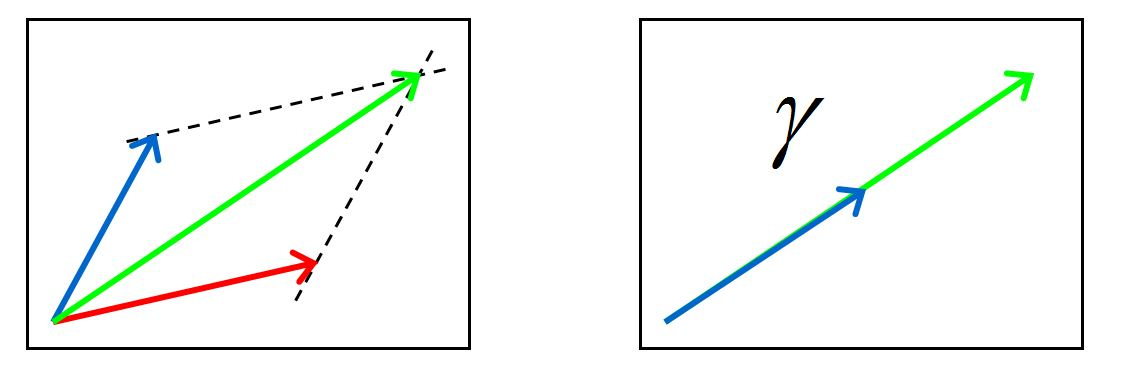
\includegraphics[width=10cm]{mat_vektory.JPG}
    \caption{(a) Sčítání vektorů (b) Násobení skalárem}
    \label{fig:mat_vektory}
\end{figure}

\subsection{Lineární zobrazení}
Zobrazení mezi vektorovými prostory X a Y tak, že zůstanou zachovány operace součtu a součinu skalárem. Patří zde lineární funkce a také Derivace a Integrace.\\
Nechť $U, V$ jsou vektorové prostory. Zobrazení $A:U\rightarrow V$ se nazývá lineární zobrazení(operátor), jestliže pro každé dva vektory $u,v \in U$ a skalár $\alpha$ platí:
\begin{enumerate}
    \item $A \cdot (u+v) = A\cdot u + A\cdot v$
    \item $A\cdot (\alpha \cdot u) = \alpha \cdot A \cdot (u)$ 
\end{enumerate}
\textbf{Superpozice} = pokud známe už výsledky x a y, tak když chceme počítat f(x+y), stačí sečíst x a y (vyplývá z definice lineárního zobrazení)\par
Nejrychlejší způsob jak zjistit zda zobrazení NENÍ lineární je podívat se, zda-li po dosazení za všechny proměnné 0, nám vyjde 0. (jelikož 0+0 = 0)... pokud ne tak to není lineární zobrazení, pokud jo, musíme dále ověřovat.\par
Každé lineární zobrazení je funkcí, ne každá funkce je lineární zobrazení. Každé lineární zobrazení lze zapsat maticí (urychluje práci, zapíšu ASAP).\\
\textbf{Zobrazení} = mapuje obraz z množiny M na vzor z množiny N\\
\textbf{Definiční obor} = množina všech vzorů\\
\textbf{Obor hodnot} = množina všech obrazů
\subsubsection{Nulový prostor/Jádro zobrazení}
Jedná se o takovou podmnožinu definičního oboru, tak že A je zobrazeno na nulový vektor. Resp. množina vzorů, jejichž obrazy jsou nulové vektory.
\subsection{Derivace reálné funkce}
Derivace nějaké funkce je změna (růst či pokles) obrazu této funkce v poměru k (ideálně) nekonečně malé změně jejích argumentů. Opačným procesem k derivování je integrování. V určitém bodě se dá derivace znázornit jako směrnice tečny (úhel) a udává nám jak se funkce mění v bezprostředním okolí. Nulová derivace v bodě znamená, že tečna je vodorovná s osou x a funkce tedy neklesá ani neroste. Jedná se o tzv. "stacionární bod", který může a nemusí mýt lokálním extrémem.\par
Derivaci můžeme derivovat znova a dostat tzv. druhou derivaci, obecně pak derivaci vyššího řádu. Logicky popisuje změnu první derivace v bezprostředním okolí. Pomocí první derivace hledáme stacionární body, potažmo jestli funkce v daném bodě klesá, či roste. Pomocí druhé derivace můžeme zjistit zda-li je stacionární bod lokálním minimem ($f'= 0$ a $f''>0$), či maximem ($f'= 0$ a $ f''<0$). Obecně sama o sobě druhá derivace udává zda-li je fce konvexní $(f''>0)$ či konkávní $(f''<0)$.

\renewcommand{\arraystretch}{1.2} 
\begin{table}[ht]
\centering
\begin{tabular}{llll}
\hline
Funkce              & Definiční obor funkce & Derivace                          & Def. obor první derivace       \\
\hline
$\displaystyle f(x) = c$          & $\mathbb{R}$          				& $\displaystyle f'(x) = 0$                       & $\displaystyle \mathbb{R}$                   \\
$\displaystyle f(x) = x^c$        & Záleží na $c$         				& $\displaystyle f'(x) = c \cdot x^{c-1}$         & Záleží na $c$                  \\
$\displaystyle f(x) = x$          & $\mathbb{R}$          				& $\displaystyle f'(x) = 1$                       &                                \\
\hline
Mocniny, logaritmy  &                       &                                   &                                \\
\hline
$\displaystyle f(x) =c^x $        & $\displaystyle \mathbb{R}$          & $\displaystyle f'(x) = c^x \cdot ln(c)$         & $\displaystyle \mathbb{R}$                   \\
$\displaystyle f(x) = e^x$        & $\displaystyle \mathbb{R}$          & $\displaystyle f'(x) = e^x$                     & $\displaystyle \mathbb{R}$                   \\
$\displaystyle f(x) = log_a(x)$   & $\displaystyle x>0$                 & $\displaystyle f'(x) = \frac{1}{x\cdot ln(a))}$ & $\displaystyle x > 0, a \neq 1, a>0$         \\
$\displaystyle f(x) =ln(x) $      & $\displaystyle x>0$                 & $\displaystyle f'(x) = \frac{1}{x}$             & $\displaystyle x > 0$                        \\
\hline
Goniometrické funkce &                       &                                   &                                \\
\hline
$\displaystyle f(x) = sin(x)$     & $\displaystyle \mathbb{R}$          & $\displaystyle f'(x) = cos(x)$                  & $\displaystyle \mathbb{R}$                   \\
$\displaystyle f(x) = cos(x)$     & $\displaystyle \mathbb{R}$          & $\displaystyle f'(x) = -sin(x)$                 & $\displaystyle \mathbb{R}$                   \\
$\displaystyle f(x) = tg(x)$      & $\displaystyle \mathbb{R}$          & $\displaystyle f'(x) = \frac{1}{cos^2(x)}$      & $\displaystyle \mathbb{R} - \frac{k \pi}{2}$ \\
$\displaystyle f(x) = cotg(x)$    & $\displaystyle \mathbb{R} - k \pi$  & $\displaystyle f'(x) = - \frac{1}{sin^2(x)}$    & $\displaystyle \mathbb{R} - \frac{k \pi}{2}$ \\
\hline
\end{tabular}
\caption{Derivace některých elementárních funkcí}
\label{tab:elementarniDerivace}
\end{table}
\renewcommand{\arraystretch}{1} 
\subsection{Určitý a neurčitý integrál}
\begin{itemize}
\item Spolu s derivací tvoří dvě hlavní operace matematické analýzy. Pojem integrálu je zobecněním pojmů jako plocha, objem, součet či suma.
\item Mějme funkci \textit{f} reálné proměnné x na intervalu [a, b]. $\displaystyle A = \int_a^b f(x) \mathrm{d}x$
\item Pod pojmem (určitý) integrál rozumíme obsah plochy ve dvojrozměrné rovině, který je omezen grafem funkce \textit{f}, osou \textit{x} a svislými přímkami \textit{x = a} a \textit{x = b}.
\begin{figure}[ht]
    \centering
    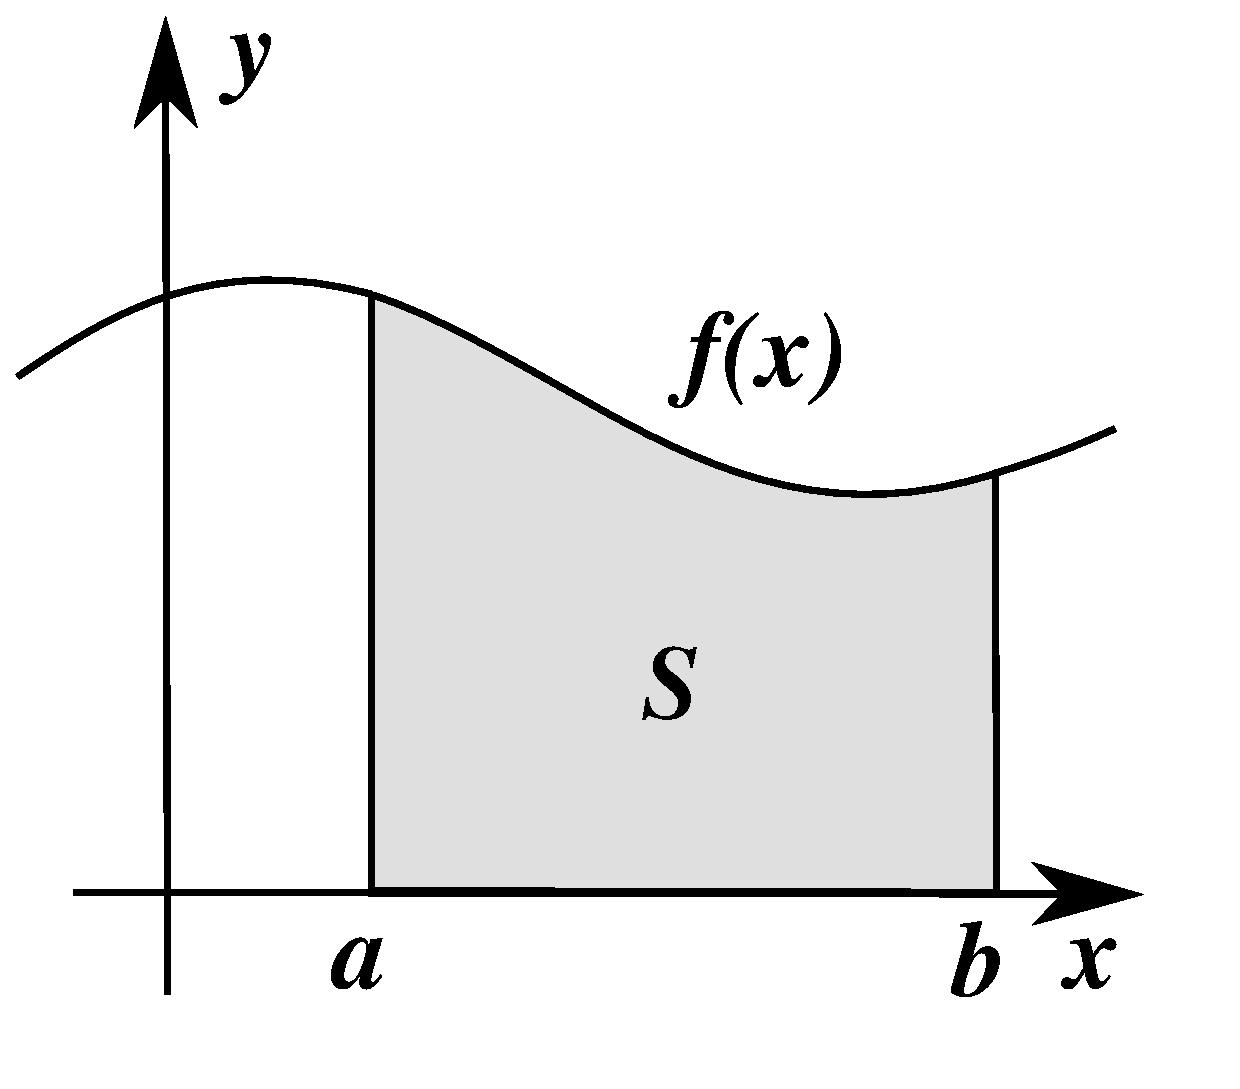
\includegraphics[width = 5cm]{Integral_as_region_under_curve.pdf}
    \caption{Ukázka určitého integrálu}
    \label{fig:Integral_as_region_under_curve}
\end{figure}
\item Neurčitý integrál je takový, který není "omezený" body a,b. Hledáme množinu funkcí, které když zderivujeme získáme původní funkci. Tuto množinu nazýváme Primitivní funkce \textit{F}. ( $\displaystyle F'(x) = f(x)$ ) a značíme $\displaystyle \int f(x)dx = F(x)+c$ 
\end{itemize}

\subsection{Kombinatorické výběry}
\renewcommand{\arraystretch}{2} 
\begin{table}[ht]
\centering
\begin{tabular}{l|l|l}
\hline
\multirow{4}{*}{Uspořádané výběry}   & Variace bez opakování   & $\displaystyle V(k, n) = \frac{n!}{(n-k)!}$ \\
                                     & Variace s opakováním    & $\displaystyle V'(k, n) = n^k$ \\
                                     & Permutace bez opakování & $\displaystyle P(n) = V(n, n) = n!$ \\
                                     & Permutace s opakováním  & $\displaystyle P'(n_1,n_2,...,n_k) = \frac{ n!}{n_1!\cdot{}n_2!\cdot{}...\cdot{}n_k!}$ \\
\multirow{2}{*}{Neuspořádané výběry} & Kombinace bez opakování & $\displaystyle C(k, n) = \frac{n!}{(n-k)!\cdot k!}$ \\
                                     & Kombinace s opakováním  & $\displaystyle C'(k, n) = \genfrac(){0pt}{0}{n+k-1}{k}$ \\ 
\hline
\end{tabular}
\caption{Vzorce kombinatorických výběrů}
\label{tab:kombVzorce}
\end{table}
\renewcommand{\arraystretch}{1} 
\begin{itemize}
\item Variace - Kolik možností jak vybrat z k prvků z n, přičemž záleží na pořadí (1,2) != (2,1)
\item Permutace - Uspořádání n prvků, nevybíráme. Opakování = některý prvek je v množině vícekrát, ale nerozlišujeme mezi nimi.(permutace = variace kde n = k)
\item Příklad bez opakování = počet různého uspořádání slova "ABC"| s opakováním = počet různého uspořádání slova "AAC".
\item Kombinace - Variace, přičemž nezáleží na pořadí = kolika možnostmi vybrat neuspořádanou k-tici z n. (1,2) = (2,1)
\item Kombinační číslo - udává počet kombinací, značíme $\displaystyle \binom{n}{k}$, čteme "n nad k". Také se nazývá binomický koeficient.
\item Pascalův trojúhelník - trojúhelník kde číslo na dalším řádku bude součtem sousedních čísel o řádek výše. Odvozený z kombinační věty.
\end{itemize}

\subsection{Grafy a jejich užití}
\subsubsection{Pojmy}
\begin{itemize}
\item \textbf{Neorientovaný graf} je dvojice G = (V,E), kde V je množina vrcholů a E je množina neuspořádaných dvouprvkových množin vrcholů = hran
\item \textbf{Orientovaný graf} je rovněž dvojice, ale E je množina uspořádaných dvouprvkových množin vrcholů.
\item \textbf{Sousední vrcholy} jsou vrcholy spojené hranou
\item \textbf{Smyčka} jedna hrana vedoucí z jednoho uzlu do sebe samého (Většinou nepovoleno v neorientovaném grafu - vzniká tzv. pseudograf)
\item \textbf{Podgraf} - Množina jeho vrcholů je podmnožinou původního a to samé platí u hran, přičemž hrana může existovat pouze mezi zahrnutými vrcholy.
\item \textbf{Faktor} - podgraf obsahující všechny jeho vrcholy (liší se pouze hranami)
\item \textbf{Stupeň vrcholu} - počet hran spojených s vrcholem, orientovaný graf má dva stupně - vstupní a výstupní
\item \textbf{Sled} - sled vrcholů a hran; začíná i končí vrcholem
\item \textbf{Tah} - sled ve kterém není žádná hrana více než jednou.
\item \textbf{Eulerův tah} - tah zahrnující všechny hrany grafu
\begin{itemize}
\item Neorientovaný souvislý graf má Eulerův tah právě když - obsahuje dva uzly lichého stupně a zbytek má stupeň sudý.
\item Orientovaný souvislý graf má Eulerův tah právě když - jeden uzel má výstupní stupeň vyšší než vstupní, výstupní stupeň o jedna nižší než vstupní a zbytek má výstupní a vstupní stupně shodné.
\item Graf obsahující Eulerův tah se nazývá Eulerův graf
\end{itemize}
\item \textbf{Eulerův okruh} - to samé co Eulerův tah, navíc končí v místě kde se začalo (Uzavřený Eulerův tah)
\begin{itemize}
\item Neorientovaný souvislý graf má Eulerův tah právě když všechny stupně mají sudý stupeň
\item Orientovaný souvislý graf má Eulerův tah právě když všechny vrcholy mají stejný vstupní i výstupní stupeň
\end{itemize}
\item \textbf{Cesta} - tah ve kterém se neopakují žádné vrcholy
\item \textbf{Hamiltonova cesta} - cesta obsahující všechny uzly
\item \textbf{Kružnice / cyklus} - Uzavřená cesta, cyklus je v orientovaném, kružnice v neorientovaném; obdobně existuje Hamiltonova kružnice
\item \textbf{Souvislost} - graf G je souvislý, jestliže pro každé jeho dva vrcholy x a y existuje v G cesta z x do y.
\item \textbf{Strom} - minimální souvislý graf bez kružnic, odebráním jakékoliv hrany se stane nesouvislým, přidáním vznikne kružnice
\item \textbf{Les} - Množina navzájem nepropojených stromů.
\item \textbf{Kořenový strom} (root tree) - orientovaný strom ve kterém je vyzačený jeden vrchol jako strom
\item \textbf{Kostra} (spanning tree) - Podgraf, který obsahuje všechny vrcholy (= faktor) a zároveň je stromem (neobsahuje kružnice)
\item \textbf{Izomorfismus grafů} - stejné grafy jinom jinak pojmenované/pokroucené.(existuje kompletní zobrazení z jednoho grafu do druhého). Stejný počet hran, vrcholů, stejné stupně, stejné sousedy...
\end{itemize}
\subsubsection{Typy grafů}
\begin{itemize}
\item \textbf{Orientovaný / neorientovaný} - orientované / neorientované hrany (popsané výše)
\item \textbf{Ohodnocený / neohodnocený} - Hrany mohou mít hodnotu (cenu), většinou slouží například ke znázornění vzdálenosti mezi městy atp., Hrany mohou mít i podmínku atp.
\item \textbf{Úplný graf} - každý vrchol spojen s každým
\item \textbf{Plánární graf(rovinný)} - graf jehož hrany se v žádném místě nekříží
\item \textbf{k - partitní graf}, který jde rozdělit na k částí tak, že vrcholy v jedné části mezi sebou nesdílí žádnou hranu. Respektive každý vrchol sousedí pouze s vrcholem z jiné skupiny. Nejčastěji nás zajímá bipartitní graf(neobsahuje liché kružnice)
\item \textbf{Síť} - orientovaný graf, kde každý vrchol má nezáporné hodnocení (x >= 0)
\item \textbf{Symetrický} - pro každý vrchol platí, že počet hran z X do Y je stejný jako z Y do X
\item \textbf{Chromatické číslo} - minimální počet barev, kterým lze graf obarvit tak, aby sousedící vrcholy neměly stejnou barvu.
\end{itemize}

\subsubsection{Algoritmy}
\begin{itemize}
\item \textbf{Kruskalův algoritmus} - vyhledávání minimální kostry grafu (přidáváme všechny hrany s co nejnižší cenou, aby nevznikla kružnice)
\item \textbf{Dijkstrův algoritmus} - vyhledávání nejkratší cesty v orientovaném grafu. Začneme na začátku, projdeme všechny hrany a aktualizujeme vzdálenost. Vezmeme vrchol s nejmenší vzdáleností a pro všechny jeho hrany aktualizujeme vrcholy. Postupujeme dokud máme jakýkoliv vrchol k projití. Výsledkem jsou nejkratší vzdálenosti do všech vrcholů v grafu vzhledem k počátku.
\item \textbf{Barvení grafů} - NP úplný problém.
\end{itemize}
\subsubsection{Užití grafu}
\begin{itemize}
\item Stromy - efektivní vyhledávání a seřazování
\item Popis relací - např. kdo je čí kamarád, co je dělitel čeho atp.
\item Nejkratší cesta - Dijkstrův algoritmus
\item Maximální tok
\item Automaty
\item "Jednotažky"
\end{itemize}
\newpage
\part{Informatika a výpočetní technika}
\newpage
\section{Úvod do teoretické informatiky}
\subsection{Interpretace a modely v predikátové logice 1. řádu. Rezoluční metoda}
\subsubsection{Interpretace a modely}
\paragraph{For experts}
\begin{itemize}
\item \textbf{Interpretace} = každému predikátovému symbolu je určena nějaká n-ární relace z daného Universa
\item \textbf{Valuace} = při dané intepretaci I s universem U je valuace funkce, přiřazující jednotlivým proměnným prvky z universa
\begin{itemize}
\item Pravdivostní hodnoty tedy přiřazujeme při dané interpretaci s daným universem a při dané valuaci
\end{itemize}
\item \textbf{Model} = Valuace při dané intepretaci, ve které je daná věta pravdivá
\end{itemize}
\paragraph{For dummies}
\begin{itemize}
\item \textbf{Interpretace} = tělo predikátu, co ten predikát vyhodnocuje
\item \textbf{Valuace} = přiřazení konkrétních hodnot do proměnných
\item \textbf{Model} = když je interpretace při nějaké valuace pravdivá, tak se jedná o model
\end{itemize}
\subsubsection{Rezoluční metoda}
\begin{enumerate}
\item Převod na CNF
\item Každá elementární disjunkce je klauzulí
\item Jedná se o důkaz sporem $\rightarrow$ znegujeme závěr a hledáme prázdnou klausuli = spor
\item Jednoliterální klauzule přiřazujeme k jiným klauzulím obsahující opačnou klauzuli a vyvozujeme nové klauzule (b a !b+c $\Rightarrow$ c)
\item Hledáme tak dlouho dokud jdou nalézt nové klauzule, nebo dokud nenajdeme prázdnou klauzuli $\perp$
\end{enumerate}
\subsection{Nedeterministické konečné automaty, uzavřenost třídy regulárních jazyků vůči různým operacím na jazycích}
\subsubsection{Nedeterministické automaty}
\begin{itemize}
\item Oproti deterministickým automatům mohou mít více počátečních stavů
\item Oproti DKA pro každý stav nemusí existovat právě tolik pravidel, kolik je velikost množiny přijímaných symbolů. Může jich být více (opakovat se), či méně, či mohou přijímat prázdné slovo.
\end{itemize}
\subsubsection{Uzavřenost regulárních jazyků}
Dříve bylo definováno co to regulární jazyk je. Jinou definicí by mohlo být, že Regulární jazyk je takový jazyk, který lze popsat konečným automatem (NDKA / DKA). Pak tedy existuje třída regulárních jazyků REG, která obsahuje všechny regulární jazyky. Při výběru x jazyků třídy REG a provedení určité operace, pak znovu dostaneme jazyk třídy REG.\\
"Uzavřenost množiny nad operací znamená že výsledek operace s libovolnými prvky z množiny bude opět spadat do dané množiny."\\
Například můžeme říci, že třída REG je užavřena vůči iteraci. Je jednoduché udělat NDKA popsující iteraci - ergo výsledný jazyk je popsatelný konečným automatem - ergo jazyk je regulární.\\
Ve zkratce - třída REG je uzavřena vůči (nekompletní výčet) - sjednocení, průniku, doplňku, zřetězení, iteraci, či např. zrcadlení
\subsection{Regulární výrazy a jejich vztah ke konečným automatům}
Řetězec popisující celou množinu řetězců, konkrétně regulární jazyk.
\paragraph{Definice regexu}
\begin{enumerate}
\item abeceda $\Sigma$
\item $\varnothing, \in, a $(kde $a \in \sigma $) jsou regulární výrazy
\item Jestliže $\alpha, \beta$ jsou regulární výrazy, pak i $(\alpha + \beta), (\alpha \cdot \beta), (\alpha*)$ jsou regulární výrazy
\end{enumerate}
U $(\alpha \cdot \beta)$ se tečka většinou nepíše (konkatenace) a může se užít přímo $\alpha \beta$.\\

Jelikož regulární výraz i konečný automat oba popisují regulární jazyk, pak můžeme říci, že každý regulární výraz lze převést na konečný automat a naopak.
\subsection{Bezkontextové jazyky a gramatiky}
Bezkontextová gramatika je formálně čtveřice $G = (\Pi, \Sigma, S, P)$
\begin{itemize}
\item $\Pi$ = množina \textbf{neterminálů} $(A,B,C...)$
\item $\Sigma$ = množina \textbf{terminálů} = samotné znaky $(a,b,c,.../1,2,3,...)$
\item $S$ = \textbf{počáteční} neterminál
\item $P$ = konečná množina přepisovacích \textbf{pravidel}
\end{itemize}
Bezkontextový jazyk = jazyk, akceptovaný tzv. zásobníkovým automatem. Jedná se o množinu jazyků jejíž podmnožinou jsou formální jazyky.\\
Bezkontextový jazyk je množina všech slov generovaná bezkontextovou gramatikou G.\\
Derivace = posloupnost odvození určitého slova v určité gramatice; rozlišujeme levou a pravou derivaci, dle směru nahrazování neterminálů\\
Derivační strom = grafická reprezentace derivace.\\
\textbf{Ekvivalence gramatik} = generují tentýž jazyk; Neexistuje slovo, které by bylo v jedné, ale ne v druhé; Algoritmicky nerozhodnutelné\\
\textbf{Nejednoznačnost gramatiky} = existují dva různé derivační stromy, jak získat určité slovo v dané gramatice.\\
\subsection{Výpočetní složitost problémů, třídy složitosti}
Viz \ref{sec:uti_slozitost} Výpočetní složitost algoritmů, asymptotická notace

\newpage
\section{Architektury počítačů, Počítačové sítě}
\subsection{Standardy IEEE 802, Ethernet. Bezdrátové sítě IEEE 802.11}
\subsubsection{Standardy IEEE 802}
IEEE 802 je skupina standardů pojednávajících o LAN sítích, mezi než patří např.:
\begin{itemize}
\item 802.2 - LLC
\item 802.3 - Ethernet
\item 802.5 - Token Ring
\item 802.11 - Wi-Fi
\end{itemize}
Definuje rozdělení 2. vrstvy OSI-RM na sublayery MAC a LLC.
\begin{itemize}
\item LLC
\begin{itemize}
\item Multiplexování. $\rightarrow$ Umožňuje, aby se v jedné síti mohlo používat několik síťových protokolů (IP, IPv6, IPX, DECnet, AppleTalk, X.25, CONS) současně.
\item zajištuje opravu chyb.
\end{itemize}
\item MAC
\begin{itemize}
\item Přístup k mediu, řešení kolizí...
\end{itemize}
\end{itemize}
\subsubsection{Ethernet} 
viz \ref{sec:ethernet}
\subsubsection{Bezdrátové sítě IEEE 802.11}
\begin{itemize}
\item Jedná se o bezdrátové sítě provozovány v pásmech 2.4 a 5 GHz.
\item Nekolik standardů 802.11-802.11ac...
\item 802.11a
\begin{itemize}
\item OFDM modulace
\item 5GHz
\item 19 kanálů
\end{itemize}
\end{itemize}
\subsection{Směrování v počítačových sítích, směrovací protokoly}
\subsubsection{Směrování obecně}
\paragraph{Circuit-switched}
\begin{itemize}
\item vyvozeno ze starých telefonních sítí
\item vytvořen kanál pro dvě strany po celou dobu komunikace
\item neefektivní
\end{itemize}
\paragraph{Packet-switched}
\begin{itemize}
\item Rozdělení dat na packety a zasílání ze zdroje do cíle
\item Neuspořádaně, každý packet mohl jít kudyma chtěl
\end{itemize}
\paragraph{Virtual channels}
\begin{itemize}
\item Kompromis mezi Circuit a Packet switched
\item Vytvoří se (virtuální) kanál jako v circuit-switched
\end{itemize}
\subsubsection{Varianty směrování}
\paragraph{Centralizované vs. Distribuované}
\begin{itemize}
\item V centralizovaném existuje centrální Routing Control Center (RCC)
\item RCC sbírá informace o routerech a počítá pro ně směrovací tabulky
\item Routery periodicky zasílají své informace do RRC
\item V distribuovaném zná každý směrovač své okolí a vyměnují si navzájem směrovací informace
\end{itemize}
\paragraph{Statické vs. Dynamické}
\begin{itemize}
\item Při statickém vytváří směrovací tabulky admin manuálně.
\item Je to bezpečnější, méně náročné na CPU, ale neadaptivní. Používá se v malých intranetech.
\item U dynamického se využívá některý z protokolů na sestrojení směrovacích tabulek.
\end{itemize}
\subsubsection{Směrovací prokotoly}
Distance Vector Algorithm (DVA) nebo Link State Algorithm (LSA).
\paragraph{DVA}
\begin{itemize}
\item Routery neznají topologie celé sítě, pouze své sousedy - next hop address
\item Směrovací tabulka je periodicky broadcastovaná sousedům (u novějších verzí pak Trigerred update)
\item Jako jednotka se udává hop count
\item Pomalá konvergence při změně topologie
\item Příklad je RIP
\end{itemize}
\paragraph{LSA}
\begin{itemize}
\item Routery znají topologii celé sítě. Tyto informace jsou pro ně uloženy v databázi.
\item Každý router spočítá nejkratší cestu do všech ostatních (Dijkstra)
\item Rychlá konvergence při změně topologie sítě
\item Příkladem je OSPF
\end{itemize}

\subsection{Topologie počítačových sítí, média, kolizní a bezkolizní metody sdílení média}
\subsubsection{Topologie}
Při topologiích hovoříme většinou LAN vs WAN topologiích.
\paragraph{LAN topologie:}
\begin{itemize}
\item Bus
\begin{itemize}
\item Jeden páteřní kabel, na obou stranách terminátor.
\item Příjem všem stanicím, malá bezpečnost
\end{itemize}
\item Star
\begin{itemize}
\item Ve středu jeden centrální prvek
\end{itemize}
\item Strom
\begin{itemize}
\item Rozšíření hvězdy - více hvězd spojeno dohromady.
\item 
\end{itemize}
\item Kruh
\begin{itemize}
\item Stanice propojeny přes medium do kruhu
\end{itemize}
\end{itemize}

\paragraph{WAN topologie:}

\begin{itemize}
\item Mesh 
\end{itemize}
 
\subsubsection{Média}
\paragraph{Metalická}

\begin{itemize}
\item Nesymetrické
\begin{itemize}
\item Koax
\begin{itemize}
\item jádro je z měděného drátu
\item odolnější vůči interferencím, ale drahé
\item Symetrické
\end{itemize}
\end{itemize}

\begin{itemize}
\item Twisted pair
\begin{itemize}
\item Typické medium v LAN sítích
\item Přenosový rychlost podle kvality kabelu (UTP cat1-8)
\item Obsahuje 4 kroucené páry drátů, - kroucení odrušuje elektrický šum
\item 2 typy - stíněná (STP) a nestíněná (UTP). U STP je všechno izolováno, samej plášť $\rightarrow$ kvalitka
\end{itemize}
\end{itemize}
\end{itemize}
\paragraph{Optická}
\begin{itemize}
\item Vysoké přenosové rychlosti, žádné elektromagnetické rušení, malá ztrátovost
\item Světlo/záření se přenáší na principu totálního odrazu - dvě rohzraní s odlišným indexem lomu
\item Typy vláken:
\begin{itemize}
\item Jednovidové
\begin{itemize}
\item Přenáší jen jeden "vid".
\item Drahé, ale nedochází k módové disperzi.
\end{itemize}
\item Mnohavidové
\begin{itemize}
\item Nízká cena, ale dochází k módové disperzi. Ta se řeší třeba Gradientním vláknem (index lomu neni stejny v hlavním vlákně).
\end{itemize}
\end{itemize}
\end{itemize}
\subsubsection{ Metody sdílení média}
\paragraph{Kolizní - CSMA/CD (Carrier Sense Multiple Access with Collision Detection)} 
\begin{enumerate}
\item Naslouchá, zda je medium volné.
\item Pokud je volné, tak zahájí vysílaní a naslouchá, jestli nepřichází signá od jiné stanice. Pokud, ano, došlo ke kolizi (více stanic může detekovat volné medium a začit vysílat). Ukončí vysílání a pošle jam signal.
\item Stanice čeká náhodnou dobu, než se pokusí znovu vysílat.
\end{enumerate}
\paragraph{Bezkolizní - CSMA/CA (Carrier Sense Multiple Access with Collision Avoidance)}
\begin{enumerate}
\item Je-li médium volné, začne vysílat, pokud druhá strana nepotvrdí příjem, tak počká a zkusí znovu.
\item Je-li medium obsazené, čeká náhodnou dobu a pak zkontroluje medium znovu.
\item Je možné využívat RTS/CTS (RTS - Request To Send - Dotaz na vysílání, CTS - Clear To Send - Volno k odeslání), před odesláním packetu samotného.
\end{enumerate}

\subsection{Monolitické počítače, základní konstrukční vlastnosti. Obvyklé integrované periférie, jejich charakteristika}
\subsubsection{Monolitické počítače, základní konstrukční vlastnosti}
Pro řadu nenáročných aplikací se vyrábějí malé počítače integrované v jediném pouzdře - tvoří tedy jeden celek $\rightarrow$ monolit.
\begin{figure}
    \centering
    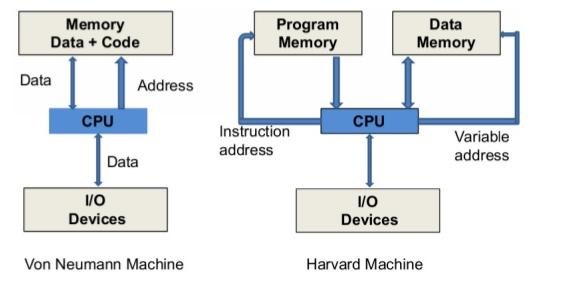
\includegraphics[width=10cm]{app_monolit-arch.png}
    \caption{Von Neumann vs Harvard}
    \label{fig:app_monolit-arch2}
\end{figure}
Využívá se většinou harvardská koncepce počítačů, tedy je oddělená pamět pro data a program. Výhoda tedy je používat odlišné technologie pamětí pro data a pro program.

\paragraph{Pro DATA}
\begin{itemize}
\item Energeticky závislé paměti (RWM-RAM)
\item Obsah není zachován po odpojení
\item Paměťová buňka realizovaná klopným obvodem
\end{itemize}


\paragraph{Pro PROGRAM}
\begin{itemize}
\item Paměti typu ROM (EPROM, FLASH EEPROM)
\item Obsah zachován i po odpojení
\end{itemize}

Podle účelu paměťové buňky můžeme v monolitických PC najít 3 základní typy pamětí:


\begin{itemize}
\item Pracovní registry
\begin{itemize}
\item pro aktuální data (výsledky operací)
\item operand strojových instrukcí
\end{itemize}
\item Univerzální zápisníkové registry
\begin{itemize}
\item ukládání nejčastěji používaných dat
\end{itemize}
\item Paměť dat RWM
\begin{itemize}
\item ukládání rozsáhlých a méně používaných dat
\item Většinou instrukční soubor nedovolí manipulaci s těmito daty, pouze jejich přesun
\end{itemize}
\end{itemize}
\paragraph{Synchronizace}
Je potřeba synchronizovat strojový a hodinový cyklus. Někdy integrovaná interně - přímo na čipu, ale díky přehřívání atp. dochází k vyšším odchylkám. Jde-li nám o přesnou dobu vykonávaná instrukcí $\rightarrow$ externí zdroj synchronizace. Ty mohou být:


\begin{itemize}
\item Křemíkový krystal
\item Keramický rezonátor
\item LC nebo RC obvod
\end{itemize}
\paragraph{RESET monolitických PC}
Je přesně definován počáteční stav počítače $\rightarrow$ označován jako RESET. Dojde k nastavení všec registrů na (většinou) 0, atp.

\paragraph{Ochrana proti rušení} 
Většinou nemáme ideální prostředí a dochází tak k rušení:

\begin{itemize}
\item Mechanické vlivy - musíme jej mít možnost bezpečně připojit k desce, musí být odolný proti vibracím a nárazům.
\item Elektromagnetické vlivy
\item Chyby programátora
\end{itemize}

\subsubsection{Obvyklé integrované periférie, jejich} charakteristika.
= obvody, které zajištují komunikaci mikropočítace s okolím.

\begin{itemize}
\item Vstupní a výstupní brány
\begin{itemize}
\item Nejjednodušší a nejčastější používané rozhraní pro vstup/výstup
\item 4 nebo 8 jednobitové vývody, kde lze současně číst i zapisovat 1/0
\end{itemize}
\item Čítače a časovače
\begin{itemize}
\item Čítač je inkrementovaný nějakým vnějším signálem
\item Časovač je inkrementován vnitřním hodinovým signálem
\end{itemize}
\item A/D, D/A převodníky - převod fyzikálních 
(ANALOGOVÝCH) veličin (napětí, proud, odpor) na (DIGITALNÍ) číselnou formu.
\end{itemize}
\subsection{Externí paměti počítačů: pevné disky, optická média. Zobrazovací jednotky: CRT, LCD, OLED, E-ink}
\subsubsection{Pevné disky}
\begin{itemize}
\item Data jsou na disku ukládána v bajtech
\item Bajty jsou uspořádány do skupin po 512 $\rightarrow$ sektor. Jedná se zároveň o nejmenší datovou jednotku, kterou lze R/W na disk.
\item Sektory jsou seskupeny do stop a stopy jsou seskupeny do cylindru.
\end{itemize}
\paragraph{Způsob R/W na HDD:}
\begin{itemize}
\item Zrealizováno pomocí směru magnetizace
\item Hlava pro čtení - nejvíc času zabere přesun hlavy, nejrychleji se tedy čtou soubory, jejichž sektory jsou na stejné stopě a stopy jsou umístěny nad sebou.
\item Hlava pro zápis - Elektrický proud prochází cívkou, vytváří tak magnetické pole, které dle směru toku magnetizuje blízké okolí (vzduchová mezera).
\end{itemize}

\subsubsection{Optická média}
\begin{itemize}
\item Pits and Lands (Jamky a ostrůvky).
\item Princip založen na odrážení paprsků - rozdílne odrážení paprsku od jamek a pevnin.
\item Stopa ve formě spirály $\rightarrow$ přehrávač musí měnit rychlost otáčení disku (CLV - constant Linear Velocity)
\item Rozdíl CD vs DVD je v rozměrech jamek a pevnin.
\end{itemize}

\subsubsection{CRT}
\begin{itemize}
\item CRTčko tvoří skleněná baňka, uvnitř které je vakuum.
\item Protože monitor je analogová technologie, tak první se digitální signál z grafiky musí převést na analogový signál, kterému bude monitor rozumět. K tomu slouží DAC konvertory(Digi to Anal convertor). Ty vytvoří "analogové tabulky", které obsahujou potřebné úrovně napětí pro zobrazení R G B barvy.
\item Na začátku baňky je elektronové dělo, které slouží jak katoda.
\item To vystřeluje pro každou ze 3 barev vysokou rychlostí proud elektronů. Ty jsou záporně nabité.
\item Vystřelování má na starosti Wheneltův válec, který je kolem katody. Má záporný potenciál a tím pádem elektrony usměrňuje do úzkého paprsku a zároveň změnou napětí dokáže regulovat množství vystřelovaných elektronů a tím pádem i jas.
\item Elektrony dál prochází sérií mřížek, které mají za úkol je dostat až k obrazovce. Mají i speciální funkce - jedna z nich (mřížka g3) elektrony ostří a další (g6) způsobuje konvergenci (pokud je špatná konvergence, tak je obraz rozostřený. Viz odkaz
\item Dál elektrony prochází kolem vychylovacích cívek. Ty určujou kam přesně na obrazovku má elektronový svazek dopadnout. Elektrony jdou postupně od levého horního rohu obrazovku k pravému, pak se přejde o řádek dolů a pokračuje zase zeva doprava. Takto se nazvývá rastrování, nebo taky řádkování.
\item Jakmile se dojde do dolního pravého rohu dokončí se jeden obnovovací cyklus (refresh). Celá cesta paprsku přes obrazovku se označuje jako "pole" 
\item Obrazovka se refreshne 60x za sekundu (klasika 60Hz obnovovací frekvence, známe i z LCD)
\item Ještě předtím, než elektron dopadne na obrazovku, tak musí projít maskou. Je to protože elektrony se navzájem odpuzujou, takže by docházelo k rozostření vysílaného svazku.
\item Maska je buď kovový plát s kruhovýma ďůrkama (nazývá se Invar a dírky jsou uspořádané do trojůhelníků) a nebo se používá(l) Trinitron. Ten to řešil tak, že maska nebyla kovový plát, ale horizontální drátky (které držely na místě ještě 2 vertiální drátky, které byly umístěné v třetinách, viz obrázek dole)
\item Maska je vyrobená z kovu, takže je náchylná na tepelnou roztažnost a působení magnetického pole. To způsobuje, že elektrony nedopadnou přímo na určené místo a zkreslujou se barvy. Řeší se to zakulacením masky (proto je sklo("obrazovka") monitoru zakulacená)
\item Jakmile elektrony projdou maskou, tak dopadají na luminofor. Je to speciální látka, která přijme energii z elektronů a vyzáří ji jako světlo. Luminofor je nanesený na obrazovku tak, že tvoří pixelovou matici. 
\end{itemize}

\subsubsection{LCD}
\begin{itemize}
\item Hlavní aktivní prvek - tekuté krystaly.
\item Polarizační filtry otočené o 90 stupňů
\item Tekuté krystaly otáči proud světla tak, aby prošlo druhým polarizačním filtrem.
\item Krystaly můžeme pomocí elektrod regulovat - podle toho kolik proudu do nich pustíme, můžeme regulovat kolik světla se dostane k barevnému filtru a tím tak vytvářet různé barvy (RGB báze).
\end{itemize}

\subsubsection{OLED}
\begin{itemize}
\item Mezi katodou a anodou jsou organické vrstvy, které při průchodu proudu z katody do anody vyzařují fotony (srážka elektronů a děr). Tento jev se nazývá rekombinace
\item Organické vrstvy jsou sami o sobě zdroj světla - není třeba podsvětlení.
\item Vysoký kontrast, velmi tenké, plně barevné, instalace i na pružný podklad, nízká spotřeba.
\end{itemize}
\subsubsection{E-ink}
\begin{itemize}
\item Jednotlivé body tvořeny kapslemi.
\item Kapsle obsahuje elektroforetický roztok.
\item V roztoku - záporně nabité černé částice (inkoust) + kladně nabité bílé částice.
\item Kapsle umístěny mezi elektrody a pomocí napětí se částice přitahují k dané elektrodě.
\end{itemize}
\subsection{Paralelní architektury grafických procesorů (např. CUDA, OpenCL, apod.)}
\subsubsection{CUDA (Compute Unified Device Architecture)}

\begin{itemize}
\item unifikovaná architektura pro (obecné) výpočty na grafických kartách
\item není potřeba znát architekturu konkrétní grafické karty, problémy se nemusí definovat v jazyce grafiky (textury), odpadá nutnost znalosti DirectX, OpenGL
\item funguje pouze na kartách od Nvidie
\item poskytuje programovací rozhraní pro často používané jazyky - C/C++, Fortran, Python
\item optimalizováno na matematicky náročné výpočty (zpracování obrazu, problémy definované pomocí mřížek), lze použít větvení, ale výkonnost programu je jím degradována
\item grafické karty obsahují velké množství ALU a malé množství řídících obvodů
\item na kartě je několik multiprocesorů (SM), každý má sdílenou paměť (+ cache na konstanty a textury), několik procesorů (každý s vlastními registry) a instrukční jednotku, která rozděluje práci procesorům
\item všechny multiprocesory mají přístup ke globální, konstantní a texturové paměti
\end{itemize}

\subsubsection{Typická operace}

\begin{enumerate}
\item Zkopírování dat z CPU na GPU
\item Spuštění vláken na GPU
\item Provedení výpočtu na GPU
\item Zkopírování výsledku z GPU na CPU
\end{enumerate}

\subsubsection{Vlákna}

\begin{itemize}
\item vlákna musí na sobě být nezávislé, nelze zaručit pořadí jejich vykonávání
\item vlákna jsou organizovány do bloku, bloky jsou dále také organizovány do mřížky (grid), lze rozšířit i do třetí dimenze
\item skupiny vláken (warpy) jsou opakovaně spouštěny schedulerem a přepínají se mezi sebou (masivní paralelismus)
\end{itemize}


\newpage
\section{Programování}
\subsection{Rekurze – ukázky rekurzívních algoritmů, složitost, metody odstranění rekurze}
Funkce, která volá sama sebe. Obsahuje podmínku pro ukončení. Klasické rekurzivní fce: faktorial, Fibonacciho posloupnost.
\subsubsection{Faktoriál}
\lstset{language=C++,
                basicstyle=\ttfamily,
                keywordstyle=\color{blue}\ttfamily,
                stringstyle=\color{red}\ttfamily,
                commentstyle=\color{green}\ttfamily,
                morecomment=[l][\color{magenta}]{\#}
}
\begin{figure}[ht]
\centering
\begin{lstlisting}
public static int faktorial(int n){
    if(n < 0) return -1;
    if(n == 0 || n == 1) return 1;
    return n * faktorial(n - 1);
}
\end{lstlisting}
\caption{Algoritmus faktoriálu s použitím rekurze}
\label{src:fakRek}
\end{figure}

\begin{figure}[ht]
\centering
\begin{lstlisting}
public static int faktorial(int n){
    int vysledek = 1;
    for(int i = 0; i < n; i++){
    vysledek *= i;
    }
    return vysledek;
}
\end{lstlisting}
    \caption{Algoritmus faktoriálu bez použití rekurze}
    \label{src:fakBezRek}
\end{figure}


\subsubsection{Fibonacciho posloupnost}
\begin{itemize}
\item Posloupnost přirozených čísel, kde každé další číslo je součtem dvou předchozích.
\item Často řešeno neefektivní rekurzivní metodou.
\end{itemize}

\begin{figure}[ht]
\centering
\begin{lstlisting}
public static int fibonacci(int index){
    if(index == 0) return 0;
    else if(index == 1) return 1;
    return fibonacci(index - 1) + fibonacci(index - 2);
}
\end{lstlisting}
    \caption{Algoritmus Fibonacciho posloupnosti s použitím rekurze}
    \label{src:fibonacciRekurze}
\end{figure}

\begin{itemize}
\item Při této rekurzivní metodě ovšem dochází k velice neefektivnímu počítání O($2^n$) a níže vidíme, že např. pro posloupnost n = 5 hodnotu 3 počítáme 2x, hodnotu 2 počítáme 3x a na triviální hodnoty (0,1) se podíváme dokonce 8x
\end{itemize}

\begin{figure}[ht]
    \centering
    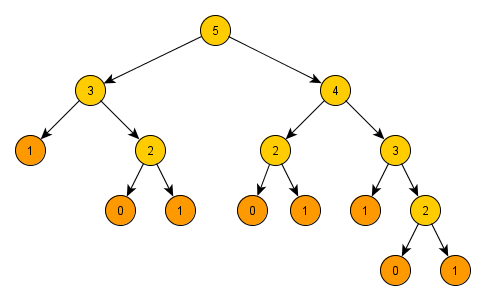
\includegraphics[width=10cm]{fibonacci.png}
    \caption{Neefektivita rekurzivního algoritmu pro Fibonacciho posloupnost}
    \label{fig:fibonacciNeefektivita}
\end{figure}

\begin{itemize}
\item Odstranění v tomto případě můžeme provést:
\begin{enumerate}
\item For cyklem, viz. kód.
\item Využitím dynamického programování - vypočítané hodnoty si uchovávat v nějaké kolekci a místo počítání hodnot, které už vypočítané máme, je pouze vytáhnout z této kolekce. Tímto stáhneme složitost z O($2^n$) na O($n$).
\end{enumerate}
\end{itemize}
\begin{figure}[ht]
\centering
\begin{lstlisting}
public static int fibonacci(int index){
    if(index == 0) return 0;
    else if(index == 1) return 1;
    int first = 0;
    int second = 1;
    int result = 0;
    
    for(int i = 1; i < index; i++){
        result = first + second;
        first = second;
        second = result;
    }
    return result;
}
\end{lstlisting}
    \caption{Algoritmus Fibonacciho posloupnosti bez použití rekurze}
    \label{src:fibonacciBezRekurze}
\end{figure}

\subsubsection{Odstranění rekurze}

\begin{itemize}
\item Většinou lze nahradit for cyklem.
\begin{enumerate}
\item Ušetříme čas za volání funkce včetně předávání parametrů
\item Pro cyklus může překladač uplatňovat optimalizace (predikce podmínky), kdežto pro rekurzivní volání ne.
\end{enumerate}
\item Rekurze se ukládá na zásobník, pro každou volanou funkci se vytvoří záznam, obsahující informace a parametry.
\item Po jejím skončení se tento záznam odebere ze zásobníku a postoupí na další.
\item Ne vždy můžeme rekurzi nahradit cyklem. Co ale funguje vždy je nahrazení rekurze vlastním zásobníkem. Na defaultní zásobník se totiž ukládá více informací, než je v některých případech potřeba.
\end{itemize}
\subsection{Stromové datové struktury – binární strom, B-strom, popis algoritmů, objasnění složitosti vybraných algoritmů}
\subsubsection{Stromové datové struktury obecně}
\begin{itemize}
\item Skládá se z kořene a vnitřních a koncových uzlů. = Root, node, leaf.
\item Konkrétní stromy mají většinou definovaný maximální počet potomků - binární, ternární, B-strom (ten má maximálně N potomků).
\item Obsahují podstromy - na každý vnitřní uzel se můžeme samostatně dívat jako na kořen vlastního ministromečku.
\end{itemize}

\paragraph{Vlastnosti:}
\begin{itemize}
\item Výška - maximální hloubka/úroveň stromu
\item Šířka - počet uzlů na jedné úrovni
\item Cesta - posloupnost uzlů od kořene k hledanému uzlu
\item Délka cesty - počet hran cesty (počet uzlů posloupnosti - 1)
\item Vyváženost - pro všechny listy platí, že nejsou o moc* hlouběji, než kterékoliv jiné listy. Nebo jinak - hloubka podstromů se liší max o x*.
\item * - přesné číslo se liší v závislostech na konkrétni implementaci, ale většinou se jedná o 1.
\end{itemize}

\paragraph{Procházení stromu}
\begin{itemize}
\item Do šířky - procházení po úrovních
\item Do výšky/hloubky - začne se v kořenu a jde se na potomka. Pokud narazíme na list nebo už byla noda navštívena, vracíme se.
\begin{itemize}
\item Podle pořadí určujeme 3 základní metody.
\item Preorder - kořen $\rightarrow$ levý podstrom $\rightarrow$ pravý podstrom
\item Inorder - levý podstrom $\rightarrow$ kořen $\rightarrow$ pravý podstrom
\item Postorder - levý podstrom $\rightarrow$ pravý podstrom $\rightarrow$ kořen
\end{itemize}
\end{itemize}

\subsubsection{Binární strom}
\begin{itemize}
\item Každý uzel má 0-2 potomky.
\item Každý uzel právě jednoho rodiče. Vyjímka samozřejmě kořen.
\item Uzly obsahují nějaký klíč, podle kterého se vyhledává. Klíče menší než kořen do levého podstromu, klíče větší než kořen do pravého podstormu.
\item Efektivní sortování a vyhledávání. U vyvážených stromů se jedná o O(log(n)). Proto je důležité mít vyvážený strom.
\end{itemize}

\paragraph{Implementace:}

\begin{itemize}
\item Dynamická struktura, tj. data a reference na levého a pravého potomka. Nevýhoda je, že máme časté ukazatele na null, když nemáme potomky a plýtváme tak paměti.
\item Pomocí pole - využíváme implicitních datových struktur (tj. data structure that uses very little memory besides the actual data elements) 
\end{itemize}
\subsubsection{B-strom}
\begin{itemize}
\item Jedná se o strom specifický tím, že má N potomků.
\item Kořen má nejvýše N potomků. Resp 2-N.
\item Vnitřní uzly jsou half-full, tedy mají N/2 až N potomků.
\item Všechny listy jsou na stejné úrovni.
\item Díky těmto vlastnostem je B-strom vyvážený, tudíž se jedná o složitost O(log(n)).
\item Vyhledávání je jednoduché, prostě to číslo porovnáváš a správně postupuješ.
\item Insert více méně to samé, ale při přetečení té nody se musí splitnout a prostřední element jde do předka.
\end{itemize}

\subsection{Implementace OOP v programovacích jazycích – popis, srovnání}

\begin{itemize}
\item C++ dovoluje třídě dědit z vícero tříd, Java jen z jedné
\item Java obsahuje interfacy - můžeme implementovat více interfejsů a jakoby napodobit vícenásobnou dědičnost ale bezpečněji
\item C++ může mít oddělené metody (program musí mít main a pak je jedno kde jsou ostatní metody), v Javě všechny metody přísluší třídě.
\item Java is Pure OOL so is C\#{}, c++ is mixture of OOL and structured language, so is python.
\item C++ statické typy, Java a c\#{} podporují generiky (dynamické typy)
\item Některé jazyky umožňují lehce měnit třídy (i za běhu?)
\item Java programátora nutí vše programovat jako OOP - všechny třídy dědí z třídy Object
\item Práce s objekty v paměti - destructor vs. Garbage Collector
\item v C++ Class neco = Objekt; v Jave Class neco = reference
\item c++ reference jsou rebindable c*++; v Jave jsou vzdy "statické" (nelze dělat aritmetiku)
\item C\#{} vs java = overloadovani operatoru v C\#{}, lepsi exception handling v c\#{} a dalsi co se daji najit v why is c\#{} the best.eu aka MSDN
\item C++ ma pointery, c\#{} ma delegata, java suší :(
\end{itemize}
Co víc k tomu chceš? Mluv o OOP a pak zmiň tady ty rozdíly. Ez.
\subsection{Java technologie, .NET technologie}
\subsubsection{Java technologie}
\paragraph{Jak Java funguje:}
\begin{itemize}
\item Java je díky JVM nezávislá na platformě (OS). Byte-code samotný je nezávislý na platformě, ale pro každou platformu existuje vlastní JVM.
\item Java compiler převadí source code na Java byte-code, který slouží pro JVM.
\item Java Runtime Environment (JRE), doplňující JVM o just-in-time (JIT) compiler, který převádí bytecode na nativní strojový kód.
\item JRE dále obsahuje Class Libraries - vzhledem k nezávislosti na platformě, nemůže spoléhat na knihovny OS, tak má vlastní na vše možné.
\item Tohle vše je obsaženo v JDK - Java Developement Kit
\end{itemize}

\paragraph{Jednotlivé technologie/platformy:}
\begin{itemize}
\item Java ME (Micro Edition)
\item Java SE (Standard edition)
\item Java EE (Enterprise edition)
\item Java FX
\end{itemize}

\paragraph{Jejich rozdíly:}
\begin{itemize}
\item Liší se především v knihovnách a různých balíčcích (SE - defines basic types and objects of the Java programming language to high-level classes that are used for networking, security, database access, graphical user interface (GUI) development, and XML parsing) a jejich využití.
\item Java ME slouží pro aplikace na zařízeních s omezenými zdroji (memory, display) jako mobily, smart TV, herní konzole.
\item Java EE rozšiřuje SE o funkce pro rozsáhlejší IS a jiné podnikové aplikace založené na více-vrstvé architektuře.
\end{itemize}

\subsubsection{.NET technologie}
\begin{itemize}
\item Soubor technologií pro web, Windows a mobilní zařízení
\item Standardizovaná specifikace jádra se nazývá Common Language Infrastructure (CLI)
\item Podobně jako u Javy lze platformu dělit dle zaměření na
\begin{itemize}
\item .NET Micro Framework - pro embedded zařízení
\item .NET Compact Framework - pro mobilní zařízení
\item .NET Framework - pro stolní PC
\item .NET Core - Multiplatformní, opensource
\end{itemize}
\item .NET podporuje více jazyků, všechny jazyky se překladačem přeloží do univerzálního kódu pro CLI
\item Nejčastější jazyky jsou C\#{}, Visual Basic .NET, Object Pascal; můžeme se setkat i s F\#, J\#, C++,...
\end{itemize}

\paragraph{Komponenty}
\begin{itemize}
\item ASP.NET - Technologie pro vývoj webových aplikací
\item WCF - Windows Communication Foundation - technologie pro vývoj webových služeb a komunikační infrastruktury (API)
\item WPF - Windows Presentation Foundation - technologie pro GUI
\item LINQ - zajišťuje objektový přístup k datům v DB, XML a IEnumerable objektech
\end{itemize}

\paragraph{Základní pojmy}
\begin{itemize}
\item CLI - definuje základní platformu pro architekturu .NET
\item CLR - Common Language Runtime - runtime pro .NET
\item CLS - Common Language Specification - společný jazyk pro .NET
\item CIL - Common Intermediate Language, dříve MSIL
\item Assembly - kus Intermediate kódu, který je určen ke spuštění CLR
\item JIT - Just In Time kompilace
\item GC - Garbage Collector - čistí paměť
\item CTS - Common Type System - společné datové jednotky pro všechny jazyky
\end{itemize}

\paragraph{Proces kompilace $\rightarrow$ spuštění}
\begin{enumerate}
\item Zdrojový kód je převeden do CIL.
\item CIL je pak převeden do bajtkódu a je vytvořeno .NET assembly.
\item Po provedení .NET assembly, jeho bajtkód projde skrz provozní JIT kompilátor, aby generoval nativní kód.
\item Nativní kód je zpracováván pomocí procesoru.
\end{enumerate}

\subsection{Skriptovací jazyky}
\subsubsection{Typické vlastnosti}Interpretovaný jazyk (nekompilovaný zdrojový kód + interpretor)
Není třeba deklarovat proměnné
Dynamická typová kontrola = automatický převod mezi řetězci, logickými hodnotami a čísly
Pokročilé datové typy, zotavení z chyb co neústí v ukončení skriptu, a další...
Program zapsaný ve skriptovacím jazyce se označuje jako skript. Typicky skript těží z výhody, že se nemusí překládat, a často tvoří rozšiřitelnou (parametrickou) část nějakého softwarového projektu, která se může měnit, aniž by bylo potřeba pokaždé rekompilovat hlavní spustitelný soubor. Skripty proto najdeme u her, složitějších softwarových řešení nebo jako hlavní součást dynamických internetových stránek a podobně. Některé programovací jazyky mají možnost kompilace do strojového kódu i interpretace; jiné umožňují i mezistupeň, předkompilování do vnitřního jazyka, jehož vykonávání je rychlejší než klasická interpretace.


\begin{itemize}
\item Typičtí zástupci = PHP, Perl, Python, Ruby, JavaScript, Lua
\end{itemize}

Některé jazyky mohou být interpretovány i kompilovány - např. Python. Některé jazyky zase mohou obsahovat nějaký mezistupeň (předkompilace) - V8 engine u Chromu předkompiluje Javascript soubory.
\subsubsection{Výhody}
\begin{itemize}
\item Není potřeba kompilovat $\rightarrow$ rychlá změna, možnost sloužit jako přídavek k hlavnímu kompilovanému programu
\item Snadnější údržba, vývoj i správa, (testování)
\item Možná intepretace kódu z řetězce za běhu
\item Netypovost
\end{itemize}

\subsubsection{Nevýhody}

\begin{itemize}
\item Není potřeba kompilovat $\rightarrow$ nutně pomalejší než předkompilovaný program
\item Netypovost $\rightarrow$ větší složitost kódu při ověřování správnosti proměnných, větší chybovost
\item Vyšší paměťová náročnost a horší přístup do paměti (větší integritní omezení)
\end{itemize}
\newpage
\section{Úvod do softwarového inženýrství}
\subsection{Softwarový proces. Jeho definice, modely a úrovně vyspělosti}
\subsubsection{Definice a dělení procesu}
"Softwarový proces je po částech uspořádaná množina kroků směřujících k vytvoření nebo úpravě softwarového díla. "

\begin{itemize}
\item Jedná se o souhrn postupů činností, které musíme provést k vytvoření softwarového produktu
\item Podle tohoto procesu pak definujeme projekty vztažené k jednotlivým zakázkám (tzv. instanciace procesu)
\item Projekt můžeme rozdělit na realizaci, vývoj a řízení. Jedná se o technickou i netechnickou část, která se řídí svou metodologii.
\item Projekt tím tak rozdělíme na metodologii realizace softwarového systému, metodologii vývoje a metodologii projektového řízení
\item Jednotlivé kroky/činnosti v procesu můžou běžet souběžně, takže je potřeba je nějakým způsobem koordinovat
\item Zároveň musí být zajištěné, že se budou dát opakovat, protože hlavní cíl je dosáhnout výsledků s konzistentní kvalitou
\item Činnosti jsou zajišťované lidmi (s danými schopnostmi, znalostmi a s technickými prostředky, které jsou potřeba pro realizaci)
\end{itemize}
\subsubsection{Úroveň vyspělosti dodavatele softwarového produktu}
Úroveň je nastavená stupnicí SEI (Software Engineering Institute). Model hodnocení má 5 stupňů a nazýváme ho CMM (Capability Maturity Model)


\begin{enumerate}
\item Počáteční (Initial) - firma nemá definován softwarový proces a každý projekt je rešen případ od případu (ad hoc)
\item Opakovatelná (Repeatable) - firma identifikovala v jednotlivých projektech opakovatelné postupy a tyto je schopna reprodukovat v každém novém projektu
\item Definovaná (Defined) - softwarový proces je definován (a dokumentován) na základě integrace dříve identifikovaných opakovatelných kroků
\item Řízená (Managed) - na základě definovaného softwarového procesu je firma schopna jeho řízení a monitorování
\item Optimalizovaná (Optimized) - zpětnovazební informace získaná dlouhodobým procesem monitorování softwarového procesu je využita ve prospěch jeho optimalizace
\end{enumerate}
\subsubsection{Modely softwarového procesu}
Dodnes neexistuje detailně a přesně definovaný referenční softwarový proces. Nicméně lze říci, že základem téměř všech se stal tzv. vodopádový model, který je možno v různých modifikacích a rozšířeních nalézt ve většině současných přístupů.
\subsubsection{Vodopádový model}

\begin{itemize}
\item Dělí SW proces na 4 základní fáze:
\item analýza požadavků a jejich specifikace, návrh softwarového systému, implementace (kódování), testování a udržování vtvořeného produktu
\item Princip vodopádu spočívá v tom, že následující množina činností spjatá s danou fází nemůže započít dříve než skončí předchozí. Jinými slovy řečeno, výsledky předchozí fáze „vtékají“ jako vstupy do fáze následující
\end{itemize}
\paragraph{Nedostatky:}

\begin{itemize}
\item Prodleva mezi zadáním projektu a vytvořením spustitelného systému je příliš dlouhá
\item Výsledek závisí na úplném a korektním zadaní požadavků kladených na výsledný produkt
\item Nelze odhalit výslednou kvalitu produktu danou splněním všech požadavků, dokud není výsledný softwarový systém hotov
\end{itemize}
\subsubsection{Inkrementální model}

\begin{itemize}
\item Jak už napovídá název, jeho nejtypičtější vlastnost je inkrementace verzí systému, které pak zahrnujou stále širší škálu funkci definovaných postupně v průběhu jeho vytváření
\item V podstatě se jedná o celou řadu menších vodopádů s výrazně kratším životním cyklem, kde každý z nich odpovídá nové sadě doplňujících požadavků
\end{itemize}
\subsubsection{Spirálový model}

\begin{itemize}
\item Zahrnuje do svého živostního cyklu další fáze jako je vytvoření a hodnocení prototypu ověřující funkcionalitu cílového systému, přičemž každý cyklus nabaluje další požadavky specifikované zadavatelem
\end{itemize}
\subsubsection{RUP (Rational Unified Process)}

\begin{itemize}
\item Definováný skupinou velkých firem, kterou koordinovala firma Rational
\item Jedná se o disciplinovaný přístup k přiřazování úkolů a zodpovědností v rámci vývojové organizace.
\item Od vodopádového modelu se liší tím, že musí dodržovat tyto principy:
\item softwarový produkt je vyvíjen iteračním způsobem (na konci každé iterace je spustitelný code, který se ověří se zadavatelem a přípomínky zpracujeme do následující iterace)
\item jsou spravovány požadavky na něj kladené (RUP popisuje jak požadavky vylákat od zadavatelů a jak je organizovat, monitorovat jejich změny a dokumentovat je)
\item využívá se již existujících softwarových komponent (komponenty se buď propojují ad-hoc (případ od případu), nebo prostřednictvím komponentní architekury - Common Object Request Broker Architecture (COBRA), Component Object Model (COM), nebo nějaká architektura využívající internet))
\item model softwarového systému je vizualizován (pomocí UML - smyslem je skrýt detaily a vytvořit kód užitím jazyka postaveného na grafickém vyjádření stavebních bloků aplikace)
\item průběžně je ověřována kvalita produktu (je obsaženo ve všech aktivitách, týká se všech účastníků vývoje softwarového řešení)
\item změny systému jsou řízeny (Řízení změn umožňuje zaručit, že každá změna je přijatelná a všechny změny systému jsou sledovatelné)
\end{itemize}

\begin{enumerate}
\item Zahájení, kde je původní myšlenka rozpracována do vize koncového produktu a je definován rámec toho, jak celý systém bude vyvíjen a implementován
\item Rozpracování je fáze věnovaná podrobné specifikaci požadavků a rozpracování architektury výsledného produktu
\item Tvorba je zaměřena na kompletní vyhotovení požadovaného díla. Výsledné programové vybavení je vytvořeno kolem navržené kostry (architektury) softwarového systému
\item Předání je závěrečnou fází, kdy vytvořený produkt je předán do užívání. Tato fáze zahrnuje i další aktivity jako je beta testování, zaškolení apod
\end{enumerate}
Každá fáze může být dále rozložena do několika iterací:
\subsubsection{Statická struktura procesu}
Smyslem procesu je specifikovat kdo v něm vystupuje, co má vytvořit, jak to má vytvořit a kdy to má vytvořit.


\begin{itemize}
\item Role (pracovníci) definující chování, kompetence a zodpovědnosti jednotlivých osob(analytik, programátor, projektový manažer apod.) nebo skupiny osob spolupracujících v týmech
\item Artefakty reprezentující entity, které jsou v procesu vytvářeny, modifikovány nebo zužitkovány (modely, dokumentace, zdrojové kódy apod.). Model je základním artefaktem (jedná se o zjednodušení reality, za účelem lepšího pochopení vyvíjeného systému)
\item Aktivity (činnosti) prováděné pracovníky s cílem vytvořit nebo upravit artefakty (kompilace zdrojových kódů, vytvoření návrhu apod.)
\item Toky (workflow) činností reprezentující posloupnosti aktivit vytvářející požadované produkty (byznys modelování, specifikace požadavků apod.)
\end{itemize}
\subsubsection{Toky procesu}
V SW procesu jsou základní toky, jejichž výsledek je artefakt (část výsledného produktu) / model, "nahlížející na vytvářeý systém z daného pohledu abstrakce (zjednodušení)" a pak podpůrné toky, které nic nevytváří ale jsou potřeba k realizaci základního roku. Základní toky jsou:


\begin{itemize}
\item Byznys modelování popisující strukturu a dynamiku podniku či organizace
\item Specifikace požadavků definující prostřednictvím specifikace tzv. případů použití softwarového systému jeho funkcionalitu
\item Analýza a návrh zaměřené na specifikaci architektury softwarového produktu
\item Implementace reprezentující vlastní tvorbu softwaru, testování komponent a jejich integraci
\item Testování zaměřené na činnosti spjaté s ověřením správnosti řešení softwaru v celé jeho složitosti
\item Rozmístění zabývající se problematikou konfigurace výsledného produktu na cílové počítačové infrastruktuře
\end{itemize}
\paragraph{Nejdůležitější podpůrné toky jsou}

\begin{itemize}
\item Řízení změn a konfigurací zabývající se problematikou správy jednotlivých verzí vytvářených artefaktů odrážejících vývoj změn požadavků kladených na softwarový systém
\item Projektové řízení zahrnující problematiku koordinace pracovníků, zajištění a dodržení rozpočtu, aktivity plánování a kontroly dosažených výsledků. Nedílnou součástí je tzv. řízení rizik, tedy identifikace problematických situací a jejich řešení
\item Prostředí a jeho správa je tok činností poskytující vývojové organizaci metodiku, nástroje a infrastrukturu podporující vývojový tým
\end{itemize}

\subsection{Vymezení fáze „sběr a analýza požadavků“. Diagramy UML využité v dané fázi}
\subsubsection{Definice}
Cílem specifikace požadavků je popsat co má softwarový systém dělat prostřednictvím specifikace jeho funkcionality. Modely specifikace požadavků slouží k odsouhlasení zadání mezi vývojovým týmem a zadavatelem
\subsubsection{Aktéři a funkční specifikace pomocí případů použití}
Modely, které jsou tvořené v rámci této činnosti vycházejí z use case případů užití. Ty tvoří:

Aktéři - definující uživatele či jiné systémy, kteří budou vstupovat do interakce s vyvíjeným softwarovým systémem
Případy užití - specifikující vzory chování realizovaných softwarovým systémem. Každý případ užití lze chápat jako posloupnost vzájemně navazujících transakcí vykonaných v dialogu mezi aktérem a vlastním softwarovým systémem.
Pro vizualizaci požadavků se používají Use Case diagramy a Sekvenční diagramy.

Use Case - popisuje vztahy mezi aktéry a jednotlivými případy použití
Sekvenční diagramy - zobrazují inerakci objektů organizovanou podle časového hlediska
\subsubsection{Use Case diagram}
Jejich smysl je zobrazit, kdo bude se systémem operovat (aktéři) a jaké funkcionalitu (případy užití) má systém mít. Vstupem pro sestavení diagramu je byznys model (konkrétně modely podnikových procesů, výsledkem jejich analýzy je seznam požadovaných funkcí).
Do takovéhohle UML ještě musíš přidat relace. Ty jsou celkem 3: (viz druhý obrázek)

Relace používá - $<<uses>>$, vyjadřuje situace kdy jeden scénář je využíván i jinými případy užití.
Relace rozšiřuje - $<<extends>>$, vyjadřuje situaci kdy nějaký scénář rozšiřuje jiný nebo "představuje variantní průchody jím popsaným scénářem"
Relace zobecnění/specializace/generalizace - vyjadřuje vztah mezi obecným scénářem a jeho speciálním případem. Zároveň vyjadřuje dědičnost u aktérů (User se dále dělí na prodejce, účetní atd)


\subsubsection{Sekvenční diagram}
Sekvenční(Iterační) diagram popisuje funkce systému z pohledu objektů a jejich iterací. Komunikace mezi objekty je znázorněna v čase, takže z diagramu můžeme vyčíst i životní cyklus. 

\subsection{Vymezení fáze „Návrh“. Diagramy UML využité v dané fázi. Návrhové vzory – členění, popis a příklady}
Návrh implementace je druhá fáze vývoje softwaru. Jde o abstrakci zdrojového kódu, která bude sloužit jako hlavní dokument programátorům v další implementační fázi.\\

V fázi návrh implementace se uplatňují tyto UML diagramy:
\begin{enumerate}
\item Diagram tříd -  statický pohled na systém zobrazuje třídy a vztahy mezi nimi. 
\item Sekvenční diagram - popisuje iterace mezi objekty v čase (viz. zde).
\item Diagram spolupráce - zaměřuje se podobně jako sekvenční na iterace mezi objekty, ale bez časové posloupnosti.
\item Stavový diagram - popisuje životní cyklus objektu a stavy ve kterých se může nacházet.
\item Diagram nasazení - popisuje konfigurací systému  (rozmístění HW a SW).
\end{enumerate}

\subsubsection{Návrhové vzory}
Návrhové vzory jsou metodiky (šablony) pro řešení různých problému, se kterými vývojář může setkat. Objektově orientované návrhové vzory typicky ukazují vztahy a interakce mezi třídami a objekty, aniž by určovaly implementaci konkrétní třídy.

Návrhové vzory se dělí do těchto 3 základních skupin:


\begin{itemize}
\item \textbf{Creational Patterns} (vytvářející) - řeší problémy související s vytvářením objektů v systému. Snahou těchto návrhových vzorů je popsat postup výběru třídy nového objektu a zajištění správného počtu těchto objektů. Většinou se jedná o dynamická rozhodnutí učiněná za běhu programu.
\item \textbf{Structural Patterns }(strukturální) - představují skupinu návrhových vzorů zaměřujících se na možnosti uspořádání jednotlivých tříd nebo komponent v systému. Snahou je zpřehlednit systém a využít možností strukturalizace kódu.
\item \textbf{Behavioral Patterns} (chování) - zajímají se o chování systému. Mohou být založeny na třídách nebo objektech. U tříd využívají při návrhu řešení především principu dědičnosti. V druhém přístupu je řešena spolupráce mezi objekty a skupinami objektů, která zajišťuje dosažení požadovaného výsledku.
\end{itemize}

\paragraph{Creational patterns (Vzory týkající se tvorby objektů)}
\begin{itemize}
\item \textbf{Abstract Factory} (Abstraktní továrna) – Definuje rozhraní pro vytváření rodin objektů, které jsou na sobě závislé nebo spolu nějak souvisí bez určení konkrétní třídy. Klient je odstíněn od vytváření konkrétních instancí objektů.
\item \textbf{Factory Method} (Tovární metoda) – Definuje rozhraní pro vytváření objektu, které nechává potomky rozhodnout o tom, jaký objekt bude fakticky vytvořen. *Tovární metoda nechává třídy přenést vytváření na potomky.
\item \textbf{Builder} (Stavitel) – Odděluje tvorbu komplexu objektů od jejich reprezentace tak, aby stejný proces tvorby mohl být použit i pro jiné reprezentace.
\item \textbf{Singleton} (Jedináček) – Potřebujete-li, aby měla třída maximálně jednu instanci.
\item \textbf{Prototype} (Prototyp, Klon) – Specifikuje druh objektů, které se mají vytvořit použitím prototypového objektu. Nové objekty se vytváří kopírováním tohoto prototypového objektu.
\item \textbf{Lazy Initialization} (Odložená inicializace) – Odkládá vytváření objektu, počítání hodnoty nebo provádění nějakého procesu, až do okamžiku, kdy je ho poprvé potřeba.
\item \textbf{Object pool} (Fond, lidově bazén) – Umožňuje vyhnout se drahému vytváření a uvolňování zdrojů recyklováním objektů, které už se nepoužívají.
\item \textbf{Multiton}
\end{itemize}


\paragraph{Structural Patterns (Vzory týkající se struktury programu)}

\begin{itemize}
\item \textbf{Adapter} (Adaptér) – Potřebujete-li, aby spolu pracovaly dvě třídy, které nemají kompatibilní rozhraní. Adaptér převádí rozhraní jedné třídy na rozhraní druhé třídy.
\item \textbf{Bridge} (Most) – Oddělí abstrakci od implementace, tak aby se tyto dvě mohly libovolně lišit.
\item \textbf{Composite} (Strom, Složenina) – Komponuje objekty do stromové struktury a umožňuje klientovi pracovat s jednotlivými i se složenými objekty stejným způsobem.
\item \textbf{Decorator} (Dekorátor) – Použijeme jej v případě, že máme nějaké objekty, kterým potřebujeme přidávat další funkce za běhu. Nový objekt si zachovává původní rozhraní.
\item \textbf{Facade} (Fasáda) – Nabízí jednotné rozhraní k sadě rozhraní v podsystému. Definuje rozhraní vyšší úrovně, které zjednodušuje použití podsystému.
\item \textbf{Flyweight} (Muší váha) – Je vhodná pro použití v případě, že máte příliš mnoho malých objektů, které jsou si velmi podobné.
\item \textbf{Proxy} – Nabízí náhradu nebo zástupný objekt za nějaký jiný pro kontrolu přístupu k danému objektu.
\end{itemize}


\paragraph{Behavioral Patterns (Vzory týkající se chování)}

\begin{itemize}
\item \textbf{Observer} (Pozorovatel) – V případě, kdy je na jednom objektu závislých mnoho dalších objektů, poskytne vám tento vzor způsob, jak všem dát vědět, když se něco změní.
\item \textbf{Command} (Příkaz) – Zapouzdřete požadavek jako objekt a tím umožněte parametrizovat klienty s různými požadavky, frontami nebo požadavky na log a podporujte operace, které jdou vzít zpět.
\item \textbf{Interpreter} (Interpret) - Vytváří jazyk, což znamená definování gramatických pravidel a určení způsobu, jak vzniklý jazyk interpretovat.
\item \textbf{State} (Stav) – Umožňuje objektu měnit své chování, pokud se změní jeho vnitřní stav. Objekt se tváří, jako kdyby se stal instancí jiné třídy.
\item \textbf{Strategy} (Strategie) – Zapouzdřuje nějaký druh algoritmů nebo objektů, které se mají měnit, tak aby byly pro klienta zaměnitelné.
\item \textbf{Chain of responsibility }(Zřetězení zodpovědnosti) – Řeší jak zaslat požadavek bez přesného vymezení objektu, který jej zpracuje.
\item \textbf{Visitor} (Návštěvník) – Reprezentuje operaci, která by měla být provedena na elementech objektové struktury. Visitor vám umožní definovat nové operace beze změny tříd elementů na kterých pracuje.
\item \textbf{Iterator} (Iterátor) – Nabízí způsob, jak přistupovat k elementům skupinového objektu postupně bez toho, abyste vystavovali vnitřní reprezentaci tohoto objektu.
\item \textbf{Mediator} (Prostředník) – Umožňuje zajistit komunikaci mezi dvěma komponentami programu, aniž by byly v přímé interakci a tím musely přesně znát poskytované metody.
\item \textbf{Memento} (Memento) – Bez porušování zapouzdření zachyťte a uložte do externího objektu interní stav objektu tak, aby ten objekt mohl být do tohoto stavu kdykoliv později vrácen.
\item \textbf{Template method} (Šablonová metoda) – Definuje kostru toho, jak nějaký algoritmus funguje, s tím, že některé kroky nechává na potomcích. Umožňuje tak potomkům upravit určité kroky algoritmu bez toho, aby mohli měnit strukturu algoritmu.
\end{itemize}

\subsection{Objektově orientované paradigma. Pojmy třída, objekt, rozhraní. Základní vlastnosti objektu a vztah ke třídě. Základní vztahy mezi třídami a rozhraními. Třídní vs. instanční vlastnosti}
Objektově-orientované programování (OOP) je metodika vývoje softwaru. Paradigma OOP popisuje způsob vývoje a zápisu programu a způsob uvažování o problému. 

\subsubsection{Základní paradigma OOP}
Při řešení úlohy vytváříme model popisované reality - popisujeme entity a interakci mezi entitami
Abstrahujeme od nepodstatných detailů - při popisu/modelování entity vynecháváme nepodstatné vlastnosti entit
Postup řešení je v řadě případů efektivnější než při procedurálním přístupu (ne vždy), kdy se úlohy řeší jako posloupnost příkazů 
\subsubsection{Cíle OOP}
Je vedeno snahou o znovupoužitelnost komponent.
Rozkládá složitou úlohu na dílčí součásti, které jdou pokud možno řešit nezávisle.
Přiblížení struktury řešení v počítači reálnému světu (komunikující objekty).
Skrytí detailů implementace řešení před uživatelem.
OOP != třídy a objekty - představuje přístup, jak správně navrhnout strukturu programu

\subsubsection{Model OOP}
OOP definuje program jako soubor spolupracujících komponent (objektů) s přesně stanoveným chováním a stavem. Metody OOP napodobují vzhled a chování objektu z reálného světa s možností velké abstrakce. Model OOP se skládá z několika následujích konstrukcí:
\paragraph{Objekt} 

Jednotlivé prvky modelované reality (jak data, tak související funkčnost) jsou v programu seskupeny do entit, nazývaných objekty. Objekty si pamatují svůj stav a navenek poskytují operace přístupné jako metody pro volání. Objekt je také instancí třídy.
\paragraph{Třída (Class)}

Třída slouží jako šablona pro vytváření instancí tříd - objektů. Seskupuje objekty stejného typu a podchycuje jejich podstatu na obecné úrovni.  (Samotná třída tedy nepředstavuje vlastní informace, jedná se pouze o předlohu; data obsahují až objekty.) Třída definuje data a metody objektů.
\paragraph{Interface (rozhraní)}

Interface předepisuje třídě, která od ní bude odvozena, jaké metody, případně properties musí implementovat. Odvozený objekt může implementovat i další metody. Interface nedefinuje žádné proměnné - pouze konstanty, ani neobsahuje naimplementované metody - obsahuje pouze abstraktní metody bez jejich implementace (jejich hlavičky). Třída může implementovat libovolný počet rozhraní (narozdíl od dědičnosti). Pokud vytvoříte rozhraní, které dědí od jiného rozhraní, automaticky tak přebírá všechny jeho metody a konstanty.
\paragraph{Abstraktní třída}

Je to takový hybrid mezi rozhraním a klasickou třídou. Od klasické třídy má schopnost implementovat vlastnosti (proměnné) a metody, které se na všech odvozených třídách budou vykonávat stejně. Od rozhraní zase získala možnost obsahovat prázdné abstraktní metody, které si každá odvozená podtřída musí naimplementovat sama. S těmito výhodami má abstraktní třída i pár omezení, a to že jedna podtřída nemůže zdědit víc abstraktních tříd a od rozhraní přebírá omezení, že nemůže vytvořit samostatnou instanci (operátorem new).

\begin{enumerate}
\item Abstraktní třída
\begin{itemize}
\item může obsahovat konkrétní metody i metody bez implementace (abstraktní)
\item lze rozšiřovat pouze jednu třídu
\end{itemize}
\item Rozhraní
\begin{itemize}
\item všechny metody jsou bez implementace
\item do jedné třídy lze implementovat více rozhraní
\end{itemize}
\end{enumerate}
\subsubsection{Rysy OOP}
\paragraph{Abstrakce} Programátor, potažmo program, který vytváří, může abstrahovat od některých detailů práce jednotlivých objektů. Každý objekt pracuje jako černá skříňka, která dokáže provádět určené činnosti a komunikovat s okolím, aniž by vyžadovala znalost způsobu, kterým vnitřně pracuje.

\paragraph{Zapouzdření (Encapsulation)}
Zaručuje, že objekt nemůže přímo přistupovat k „vnitřnostem“ jiných objektů, což by mohlo vést k nekonzistenci. Každý objekt navenek zpřístupňuje rozhraní, pomocí kterého (a nijak jinak) se s objektem pracuje.

\paragraph{Skládání}
Objekt může obsahovat jiné objekty.

\paragraph{Delegování}
Objekt může využívat služeb jiných objektů tak, že je požádá o provedení operace.

\paragraph{Dědičnost (Inheritance)}
objekty jsou organizovány stromovým způsobem, kdy objekty nějakého druhu mohou dědit z jiného druhu objektů, čímž přebírají jejich schopnosti, ke kterým pouze přidávají svoje vlastní rozšíření. Tato myšlenka se obvykle implementuje pomocí rozdělení objektů do tříd, přičemž každý objekt je instancí nějaké třídy. Každá třída pak může dědit od jiné třídy (v některých programovacích jazycích i z několika jiných tříd).

\paragraph{Polymorfismus}
odkazovaný objekt se chová podle toho, jaké třídy je instancí. Pokud několik objektů poskytuje stejné rozhraní, pracuje se s nimi stejným způsobem, ale jejich konkrétní chování se liší podle implementace. U polymorfismu podmíněného dědičností to znamená, že na místo, kde je očekávána instance nějaké třídy, můžeme dosadit i instanci libovolné její podtřídy. U polymorfismu nepodmíněného dědičností je dostačující, jestliže se rozhraní (nebo jejich požadované části) u různých tříd shodují, pak jsou vzájemně polymorfní. Polymorfismus bývá často vysvětlován na obrázku se zvířaty, která mají všechna v rozhraní metodu Speak(), ale každé si ji vykonává po svém. 
\paragraph{Genericita}
Je možnost programovaciho jazyka definovat místo typů jen „vzory typů“, kde typy proměnných, použité v definici (ADT typy) jsou vyvedeny vně definice jako parametry a jsou určeny později klientskou aplikací.
\subsubsection{Třídní vs. instanční vlastnosti}
Instanční proměnné
\begin{itemize}
\item udávají vlastnosti objektů
\item přístup ze třídy nebo pomocí metod get() a set()
\item vznikají s objektem
\end{itemize}
Statické proměnné
\begin{itemize}
\item nepopisují vlastnosti objektů
\item existují pouze jednou pro třídu
\item mohou existovat bez objektu
\item přístup ze třídy nebo pomocí jména třídy
\end{itemize}
\subsection{Mapování UML diagramů na zdrojový kód}
K mapování UML diagramů na kód dochází v první části implementační fáze vývoje. Jde o automatické vygenerování zdrojového kódu z UML diagramu. \\
Z diagramu tříd například vygeneruje jednotlivé rozhraní, třídy s proměnnými a prázdnými metodami.\\
Z diagramů komponent pak vyčte a do generovaného kódu přidá požadované komponenty. Komponenta je už existující a vyměnitelná část systému s daným rozhraním skrze které jí systém používá. Jde o komponentu napsanou v zdrojovém kódu, nebo už zkompilovanou komponentu v binárním kódu, či další komponenty reprezentovanými databázovými tabulkami, dokumenty, apod. \\
Úkolem samotné implementace je pak dopsat těla metod, jejichž chování může být popsáno v diagramu aktivit.
\subsection{Správa paměti (v jazycích C/C++, JAVA, C\#, Python), virtuální stroj}
Správa paměti je v informatice soubor metod, které operační systém používá při přidělování operační paměti jednotlivým spuštěným procesům. \\
V jazyce Java i C\# je správa paměti plně automatizovaná. O uvolňování paměti se stará separátní vlákno, které běží s nízkou prioritou a zajišťuje kontinuální sledování nepoužitých bloků paměti. Přidělování paměti se provádí operátorem new.
\subsubsection{Úrovně správy paměti}

\begin{itemize}
\item Technické vybavení
\begin{itemize}
\item registry, cache
\end{itemize}
\item Operační systém
\begin{itemize}
\item virtuální paměť
\item segmentace, stránkování
\end{itemize}
\item Aplikace
\begin{itemize}
\item Přidělování paměti
\item Regenerace paměti
\begin{itemize}
\item Manuální – delete, dispose, free(), …
\item Automatická – garbage collection
\end{itemize}
\end{itemize}
\end{itemize}
\paragraph{Garbage collector (GC)} je obvykle část běhového prostředí (programovacího) jazyka, nebo přídavná knihovna, podporovaná kompilátorem, hardware, operačním systémem, nebo jakoukoli kombinací těchto tří. Má za úkol automaticky určit, která část paměti programu je už nepoužívaná, a připravit ji pro další znovupoužití.
\subsubsection{Virtuální stroj}
Virtuální stroj je v informatice software, který vytváří virtualizované prostředí mezi platformou počítače a operačním systémem, ve kterém koncový uživatel může provozovat software na abstraktním stroji.
\paragraph{Hardwarový virtuální stroj}
Původní význam pro virtuální stroj, někdy nazývaný též hardwarový virtuální stroj, označuje několik jednotlivých totožných pracovních prostředí na jediném počítači, z nichž na každém běží operační systém. Díky tomu může být aplikace psaná pro jeden OS používána na stroji, na kterém běží jiný OS, nebo zajišťuje vykonání sandboxu, který poskytuje větší úroveň izolace mezi procesy než je dosaženo při vykonávání několika procesů najednou (multitasking) na stejném OS.\\
Jedním využitím může být také poskytnutí iluze mnoha uživatelům, že používají celý počítač, který je jejich „soukromým“ strojem, izolovaným od ostatních uživatelů, přestože všichni používají jeden fyzický stroj. Další výhodou může být to, že start (bootování) a restart virtuálního počítače může být mnohem rychlejší, než u fyzického stroje, protože mohou být přeskočeny úkoly jako například inicializace hardwaru.\\
Podobný software je často označován termíny jako virtualizace a virtuální servery. Hostitelský software, který poskytuje tuto schopnost je často označovaný jako hypervisor nebovirtuální strojový monitor (virtual machine monitor).
\paragraph{Aplikační virtuální stroj}
Dalším významem termínu virtuální stroj je počítačový software, který izoluje aplikace používané uživatelem na počítači. Protože verze virtuálního stroje jsou psány pro různé počítačové platformy, jakákoliv aplikace psaná pro virtuální stroj může být provozována na kterékoli z platforem, místo toho, aby se musely vytvářet oddělené verze aplikace pro každý počítač a operační systém. Aplikace běžící na počítači používá interpret nebo Just in time kompilaci.\\
Jeden z nejlepších známých příkladů aplikace virtuálního stroje je Java Virtual Machine od firmy Sun Microsystem. Java Virtual Machine umí zpracovat mezikód (Java bytecode), který je obvykle vytvořen ze zdrojových kódů programovacího jazyka Java. Díky tomu že je JVM k dispozici na mnoha platformách, je možné aplikaci v Javě vytvořit pouze jednou a spustit na kterékoliv z platforem, pro kterou je vyvinut JVM (např. Windows, Linux).
\subsection{Podpora paralelního zpracování, vlákna}
\subsubsection{Paralelní zpracování}
\begin{itemize}
\item Rozdělení nějaké úlohy na dílčí části a ty spustíme zároveň
\item Tím pádem nám ale vznikají nové nebezpečí programování, na které si musíme dát pozor - např. souběh
\item Souběh znamená, že dílčí části přistupují k např. proměnné současně a bijou se mezi s sebou.
\item Dá se to řešit, několika způsoby, nejideálněji proramovat takovým způsobem, aby k souběhu nedocházelo
\item Pokud je to ovšem nezbytně nutné a k souběhu docházet bude, musíme použít např. TSL (Test and Set Lock)
\end{itemize}
\subsubsection{Vlákna}
\begin{itemize}
\item Tady ty dílčí části (definované u paralelního zpracování) ovládá jedno nějaké vlákno
\item "Samostatně prováděny výpočetní, který běží v rámci jednoho procesu."
\item Konkrétně v Javě dva způsoby:
\begin{itemize}
\item Implementováním interfejsu Runnable.
\item Deděním z třídy Thread.
\item Oba způsoby vyžadují implementaci funkce Run() - čili co se bude ve vlákně dít.
\item Druhý způsob nabízí větší flexibilitu při handlování vícero vláken.
\end{itemize}
\end{itemize}
\subsubsection{Vlákna v Javě}
Každé vlákno v Javě je instancí třídy \texttt{java.lang.Thread}. Tato třída zajišťuje spuštění, zastavení a ukončení vlákna. Vlákno musí implementovat metodu run, která definuje činnost vlákna. Této metodě je předáno řízení po spuštění vlákna metodou start.
\paragraph{Životní cyklus} 
Vlákno v průběhu svého života prochází posloupností následujících stavů:
\begin{itemize}
\item \textbf{New} - bezprostředně po vytvoření ještě nejsou vláknu přiděleny žádné systémové prostředky, vlákno neběží.
\item \textbf{Runnable} - po provedené metody start je vlákno připraveno k běhu. V tomto stavu se může nacházet více vláken, ovšem jen jedno z nich (na počítači s jedním procesorem) je ve stavu „běžící“.
\item \textbf{Not runnable} - do tohoto stavu se vlákno dostane, je-li pozastaveno voláním jedné s metod sleep, wait nebo suspend, případně čekáním na dokončeníoperace vstupu/výstupu.
\item \textbf{Dead} - do tohoto stavu se vlákno dostane ukončením metody run nebo voláním metody stop.
\end{itemize}
\paragraph{Vícevláknové aplikace a ladění}
Hlavní problémy vícevláknových aplikací souvisí se synchronizací
\begin{itemize}
\item uváznutí - Deadlock - je situace, kdy úspěšné dokončení první akce je podmíněno předchozím dokončením druhé akce, přičemž druhá akce může být dokončena až po dokončení první akce. Deadlocku můžeme zabránit například tím, že proces musí o všechny prostředky, které potřebuje, zažádat najednou. Buď je všechny dostane, nebo nedostane ani jeden. 
\item souběh (race conditions) - přístup více vláken ke sdíleným proměnným a alespoň jedno vlákno nevyužívá synchronizačních mechanismů. Vlákno čte hodnotu zatímco jiné vlákno zapisuje. Zápis a čtení nejsou atomické a data mohou být neplatná. K zabránění souběhu se používají zámky (lock), jejichž použitím se zajistí, že jen jedno vlákno může v jeden okamžik přistoupit k označenému resource souboru nebo části kódu.
\item vyhladovění - Vyhladovění - stav, kdy jsou vláknu neustále odepírány prostředky. Bez těchto prostředků program nikdy nedokončí svůj úkol.
\end{itemize}
\subsection{Zpracování chyb v moderních programovacích jazycích}
Výjimky představují určité situace, ve kterých musí být výpočet přerušen a řízení předáno na místo, kde bude provedeno ošetření výjimky a rozhodnutí o dalším pokračování výpočtu. Starší programovací jazyky pro ošetření chyb během výpočtu obvykle žádnou podporu neměly. U všech funkcí, které mohly objevit chybu, bylo třeba stále testovat různé příznaky a speciální návratové hodnoty, kterými se chyba oznamovala, a v případě, že jsme na testování chyby zapomněli, program běžel dál a na chybu v nejlepším případě nereagoval nebo se zhroutil na zcela jiném místě, kde již bylo obtížné zdroj chyby dohledat. \\
Jazyk Java, podobně jako např. C++, využívá pro ošetření výjimek metodu strukturované obsluhy. To znamená, že programátor může pro konkrétní úsek programu specifikovat, jakým způsobem se má konkrétní typ výjimky ošetřit. V případě, že výjimka nastane, vyhledá se vždy nejbližší nadřazený blok, ve kterém je výjimka ošetřena. \\
Výjimky jsou v jazyce Java reprezentovány jako objekty...tyto objekty jsou instancemi tříd odvozených obecně od třídy Throwable se dvěma podtřídami Error a Exception. Každá z těchto podtříd odpovídá jedné skupině výjimek. V první skupině jsou výjimky, jejichž výskyt představuje vážný problém v činnosti aplikace a které by programátor neměl zachycovat. Druhou skupinu tvoří výjimky, jejichž ošetření má smysl - jde například o výjimky jako pokus o otevření neexistujícího souboru, chybný formát čísla apod. Do této skupiny by měly patřit také veškeré výjimky definované uživatelem.
\paragraph{Příkaz try-catch}
Zpracování výjimky se vždy vztahuje k bloku programu omezenému příkazem try následovaném jedním nebo více bloky catch popisujícími způsob ošetření jednotlivých výjimek. \\
Potřebujeme-li vyvolat v programu vlastní výjimku, je třeba nejprve vytvořit vhodnou třídu, odvozenou od třídy Exception nebo některé její podtřídy.
\subsection{Princip datových proudů – pro vstup a výstup. Rozdíl mezi znakově a bytově orientovanými datovými proudy}
Datové proudy (dále jen proudy) jsou sekvence dat. Proud je definován svým vstupem a výstupem, těmi mohou být například soubor na disku, zařízení (vstupní klávesnice nebo myš, výstupní displej) nebo jiný program.
\paragraph{Vstupně–výstupní zařízení (I/O):}
\begin{itemize}
\item znakové: vstupní – klávesnice, výstupní – monitor, tiskárna.
\item bloková: pevný disk,flash disk, SD, microSD
\end{itemize}
Z klávesnice čteme sekvenčně znak po znaku (\textbf{sekvenční přístup}), u binárního diskového souboru můžeme libovolně přistupovat ke zvolené části dat – \textbf{náhodný přístup}.\\
Primitivní proudy pouze přenášejí binární data, specializované proudy umí s přenášenými daty manipulovat. Tyto manipulační schopnosti se liší podle typu přenášených dat.
\paragraph{Typy přenášených informací:}
\begin{itemize}
\item binární data – obrázky, zvuk, objekty, ... - data uložené ve stejné formě v jaké jsou uloženy v počítači
\item textová data – představují řádky textů v ASCII nebo UNICODE
\end{itemize}
\subsubsection{Typy proudů}
\paragraph{Znakové proudy}
\begin{itemize}
\item posloupnost 16-bitových znaků UNICODE
\item rozhraní: java.io.Reader, java.io.Writer
\item FileReader - čte data char po charu (implicitně 16bitů, ale lze specifikovat i kodování)
\end{itemize}

\paragraph{Bajtové proudy}
\begin{itemize}
\item proud čte nebo zapisuje data na nízké úrovni po 8 bitových svazcích.
\item rozhraní:  java.io.InputStream, java.io.OutputStream
\item FileInputStream - čte data byte po bytu.
\item Nejvíc low-level. Pokud víme, že soubor, který čteme, bude třeba text a chceme pracovat s textem, je lepší použít specifikovanější Streamy
\end{itemize}

\paragraph{Proudy s vyrovnávací pamětí}
\begin{itemize}
\item čtení/zápis s využitím vyrovnávací paměti
\item rozhraní:  BufferedReader/ BufferedWriter 
\item BufferedReader - pouze obaluje jiné InputStreamy
\item Nečte data po charu/bytu po každé z (např.) disku, místo toho je \item přenese do vyrovnávací paměti a pak čte
\item Díky tomu je rychlejší a efektivnější
\end{itemize}

\paragraph{Datové proudy}
Java obsahuje třídy pro pohodlné čtení a zápis primitivních datových typů a typu String. Nejrozšířenější třídy jsou DataInputStream a DataOutputStream. String je ukládán v kódování UTF-8. Údaje takto uložené např. do souboru nejsou uživatelsky přívětivé a s výjimkou řetězců čitelné. Metody pro čtení jsou readDouble, readInt, readUTF. Obdobně metody pro zápis mají předponu write.

\paragraph{Objektové proudy}
Většina standardních tříd implementuje rozhraní Serializable (serializovatelný), které je nezbytné pro jejich podporu objektovými proudy. Objektové proudy rozšiřují datové proudy, takže objektové proudy umí pracovat i s primitivními datovými typy. Nové metody jsou readObject a writeObject. Pokud metoda readObject vrátí jiný než očekávaný objekt, vyhodí výjimku typu ClassNotFoundException. Pokud se objekt neskládá jen z primitivních typů ale i z referencí na další objekty, je potřeba zachovat tyto reference. Proto je při zápisu objektu uložit i všechny objekty, na které má daný objekt odkaz. Podobně se bude chovat čtecí proud, který se bude snažit zrekonstruovat celou takovou síť objektů
\subsection{Jazyk UML – typy diagramů a jejich využití v rámci vývoje}
\subsubsection{UML}
UML je jednotný jazyk pro tvorbu diagramů. Definuje standardy pro jednotnou strukturu diagramů. Pomocí něj můžeme realizovat nejrůznější schemata napříč procesem vývoje softwaru .\\
UML jazyk umožňuje specifikaci (struktura a model), vizualizaci (grafy), konstrukci (vygenerování kódu např. z class diagramu) a dokumentaci artefaktů softwarového systému.\\
Každý z UML diagramů se také používá v jiné fázi vývoje softwaru. 
\subsubsection{Dělení UML}
Postihující různé aspekty systému:
\begin{enumerate}
\item Funkční náhled
\begin{itemize}
\item Diagram případů užití (Use case)
\end{itemize}
\item Logický náhled
\begin{itemize}
\item Diagram tříd
\item Objektový diagram
\end{itemize}
\item Dynamický náhled popisující chování
\begin{itemize}
\item Stavový diagram
\item Diagram aktivit
\item Interakční diagramy
\item Sekvenční diagramy
\item Diagramy spolupráce
\end{itemize}
\item Implementační náhled
\begin{itemize}
\item Diagram komponent
\item Diagram nasazení
\end{itemize}
\end{enumerate}

\subsubsection{Třídní diagram}
diagram struktury tříd poskytuje logický náhled na systém. Znázorňuje datové struktury, operace u objektů a také jejich vazby. Třídní diagram se využívá pro tvorbu ERD a při návrhu implementace.
\paragraph{Typy vazeb v třídním diagramu}
\begin{enumerate}
\item Agregace
\begin{itemize}
\item vztah vyjdařující katedra má profesory, zánik department neznamená zánik professor
\end{itemize}
\item Kompozice
\begin{itemize}
\item nejsilnější asociace, existence odkazovaného objektu (department) bez majitele (faculty) nemá smysl a zaniká i s ním
\end{itemize}
\item Realizace
\begin{itemize}
\item implementace rozhraní
\end{itemize}
\item Generalizace
\begin{itemize}
\item dědičnost - automobil dědí z vehicle
\end{itemize}
\item Asociace
\begin{itemize}
\item vztah mezi instancemi - posílají si zprávy
\end{itemize}
\item Závislost
\begin{itemize}
\item třída animal používá třídu food (je na ni závislá)
\end{itemize}
\end{enumerate}
\subsubsection{Objektový diagram}
zobrazuje instance tříd - objekty, někdy nazýván jako instanční diagram.
Je snímkem objektů a jejich vztahů v systému v určitém časovém okamžiku, který chceme z nějakého důvodu zdůraznit. Využívá se v datové analýze pro ERD.
\subsubsection{Diagram případu užití}
poskytuje funkční náhled systému (kdo se systémem pracuje a jak). 
Uplatňuje se pro realizaci DFD, ve vývojové fázi specifikace požadavků.
\subsubsection{Stavový diagram}
zobrazuje životní cyklus objektů a stavy do kterých se během svého života dostávají. Obsahuje 3 základní prvky – stav, událost, přechod. Využívá se při návrhu implementace. 
\subsubsection{Diagram aktivit}
grafické znázornění algoritmů. Tento diagram se používá pro modelování procedurální logiky, procesů a zachycení workflow. Každý proces v diagramu aktivit je reprezentován sekvencí jednotlivých kroků, které určují řídící tok. Tento diagram obsahuje i rozhodovací symbol (kosočtverec) s podmínkou, kdy tok procesu pokračuje na základě odpovědi jednou z větví.
Diagram aktivit se využívá pro tvorbu minispecifikací a dalších podrobných analýz a při specifikaci požadavků.
\subsubsection{Sekvenční diagram}
Sekvenční diagram (Sequence diagram) znázorňuje komunikaci mezi objekty v čase.\\
Používá se ve vývojové fázi specifikace požadavků a návrhu implementace.
\subsubsection{Diagram spolupráce} 
dynamický pohled na systém znázorňující chování objektů v systému. Diagram spolupráce upřednostňuje při popisu vzájemné komunikace mezi objekty jejich topologii, tedy jejich rozložení a vzájemné spojení. Podobný jako sekvenční ale bez času. Využití  v implementační fázi.
Časová posloupnost zaslání zpráv je vyjádřena jejich pořadovým číslem. Návratová hodnota je vyjádřena operátorem přířazení :=. Opakované zaslání zprávy je dáno symbolem * a v hranatých závorkách uvedením podmínky opakování cyklu. Navíc tento diagram zavádí i následující typy viditelnosti vzájemně spojených objektů: 
\begin{itemize}
\item $<<local>>$ vyjadřuje situaci, kdy objekt je vytvořen v těle operace a po jejím vykonání je zrušen; 
\item $<<global>>$ specifikuje globálně viditelný objekt; 
\item $<<parameter>>$ vyjadřuje fakt, že objekt je předán druhému jako argument na něj zaslané zprávy; 
\item $<<association>>$ specifikuje trvalou vazbu mezi objekty (někdy se také hovoří o tzv. známostním spojení).
\end{itemize}
\subsubsection{Diagram komponent}
ilustruje organizaci a závislosti mezi softwarovými komponentami. Zdrojové komponenty tvoří soubory vytvořené použitým programovacím jazykem. Diagram spustitelných komponent specifikuje všechny komponenty vytvořené námi i ty, které nám dává k dispozici implementační prostředí.
\subsubsection{Diagram nasazení}
upřesněný nejen ve smyslu konfigurace technických prostředků, ale především z hlediska rozmístění implementovaných softwarových komponent na jednotlivé technické prostředky reprezentované v počítači.
\subsection{Struktura a činnost překladače, tvar zdrojového a cílového programu. Interpretační a kompilační překlad. Fáze překladu, vnitřní struktura překladače}
\subsubsection{Překladač}
Překladač je program, který překládá programy z jednoho programovací jazyka do jiného. Překladač tedy přečte zdrojový program napsaný v zdrojovém jazyce přeloží ho do ekvivalentního programu (cílový program), který je však napsaný v jiném (cílovém) jazyce. \par
Překladače využívají i vyšší programovací jazyky jako Prolog, Lips, apod.  Překladače se také uplatnily všude tam, kde je třeba pochopit význam textu (sémantická analýza). Například strukturované editory, automatické doplňovače kódu (doplnění závorek), formátovací a sázecí programy (\LaTeX).\par
Důležitým prvkem překladače jsou diagnostické zprávy které informují o chybách ke kterým během překladu došlo a s kterými si překladač neporadil.\\
Podle přístupu k překladu dělíme překladače na
\begin{itemize}
\item \textbf{Kompilátory} (kompilační překladače)  - přeloží kód zdrojového program na kód v cílovém jazyce, který je následně spuštěn a vykonán. Výhodou těchto kompilátorů je, že program se přeloží jednou a dál už se spouští jen cílový program.
\item \textbf{Interprety} (interpretační překladače) - oproti tomu interpreti vynechávají krok vytvoření cílového programu a zdrojový program překládají rovnou do akcí, které se vykonávají. Viz. obrázek vpravo.
\end{itemize}
Podle závislosti na architektuře počítače dělíme cílové programy na:
\begin{itemize}
\item \textbf{čistý strojový kód} - obsahuje jen instrukce instrukčního souboru počítače, nepředpokládá existenci operačního systému (OS) a je tedy plně závislý na konkrétní HW.
\item \textbf{rozšířený strojový kód} - využívá kromě instrukčního souboru počítače i podprogramy OS. Je tedy závislý jak na hardwaru tak na softwaru počítače. Překladač Fortranu.
\item \textbf{virtuální strojový kód} - obsahuje pouze virtuální instrukce, které nejsou závislé ani na HW ani na SW počítače. Díky tomu jsou překladatele přenositelné, stačí jen dopsat interpreta virtuálního kódu.
\end{itemize}
Podle formátu dělíme cílový kód na:
\begin{itemize}
\item \textbf{Symbolický formát} - klasický zdroják s instrukcemi v kterých se člověk vyzná. Nejčastěji se jedná o assembler.
\item \textbf{Relokativilní binární formát} - kód v binárním tvaru, ale bez vyřešených odkazů na externí symboly. Adresy jsou relativní od nějakého počátečního úseku.
\item \textbf{Absolutní binární formát} - binární spustitelný kód.
\end{itemize}
\subsubsection{Struktura překladače}
Překladač provádí dvě základní činnosti - analyzuje zdrojový kód a následně jej přeložit do cílového programu. Součástí analýzy je lexikální, syntaktická a strukturální analýza.

Činnost překladače je následující: Zdrojový kód $\rightarrow$ pre-procesor $\rightarrow$ lexikální analyzátor $\rightarrow$ syntaktický analyzátor $\rightarrow$ tvorba mezikódu $\rightarrow$ optimalizátor $\rightarrow$ generování výsledného kód $\rightarrow$ optimalizace závislá na zařízení.\\
Součástí generování cílového programu je optimalizace kódu. 
\paragraph{Lexikální analýza}
Text zdrojového kódu přepisuje lexikální analyzátor na posloupnost lexikálních jednotek (lexémů), tedy výrazu mající význam jako identifikátor (proměnná), operátor, symbol přiřazení. apod.\\
Tyto lexémy jsou reprezentovány ve formě tokenů, které jsou poskytnuty ke zpracování syntaktickému analyzátoru. Úkolem lexikálního analyzátoru je také odstranění komentářů a bílých znaků ze zdrojového programu. \\
Funkce lexikálního analyzátoru:
\begin{enumerate}
\item nalezení a rozpoznání lexikálního symbolu
\item zakódování lexikálních symbolů,
\item vynechání nepotřebných znaků a symbolů
\item výpočet syntetizovaných atributů lexikálních symbolů.
\end{enumerate}
V praxi je lexikální analyzátor realizován pomocí konečného automatu.
\paragraph{Syntaktická analýza}
Syntaktická analýza převede lexikální jednotky na fráze. Ty se obvykle reprezentují derivačním stromem. V této fázi se využívají bezkontextové gramatiky, které z výrazu sestrojí derivační stroj.\\
Vstupem jsou tedy tokeny (např. závorka, literál, proměnná, klíčové slovo, symbol a pod.), což je pro parser již dále nedělitelná základní stavební jednotka, které má uloženy v listech načteného datového stromu.
\paragraph{Sémantická analýza}
Sémantická analýza postupně prochází symboly či skupiny symbolů získané ze syntaktické analýzy a přiřazuje se jim význam. Pokud například skupina symbolů představuje použití konkrétní proměnné, pak analyzátor zjišťuje zda je proměnná už deklarována (pokud je to požadováno, nevyžaduje například programovací jazyk Perl či PHP) a zda je správně použita vzhledem k jejímu datovému typu. Dále například u operací kontroluje zda jsou operandy správného typu, případně provede potřebnou konverzi datového typu. \\
Sémantická analýza tedy zpracovává především deklarace, které ukládá do svých datových struktur dělá se zde typová kontrola a další kontroly které ověřují, zda kód odpovídá specifikaci zdrojového jazyka. 

\paragraph{Generování mezikódu}
Některé překladače generují mezikód (explicitní intermediální reprezentaci kódu). Jde o jakýsi kód pro abstraktní počítač, který lze jednoduše vytvořit a zároveň jej i jednoduše převést do cílového kódu. Pro některé interpretační překladače jde o poslední fázi a mezikód už rovnou vykonávají.\\
Mezikódy v této fázi mohou mít různé podoby jednou z nich je tříadresový kód který vidíte v příkladu vpravo. Tříadresový kód se podobá instrukcím pro počítač a sestává se s posloupnosti instrukcí o nanejvýš třech operandech.
\paragraph{Optimalizace kódu}
Vylepšuje kód tak aby byl rychlejší nebo kratší. Některé optimalizační metody jsou triviální, například zjednodušení různých výpočtů a zredukování proměnných intermediálního kódu jak je ukázané na příkladu vpravo.
\paragraph{Generování cílového kódu}
Posledním krokem překladače je vygenerování cílového kódu. Výsledkem je většinou přemístitelný strojový kód, nebo program v asembleru. V této fázi se všem proměnným přidělí místo v paměti a instrukce mezikódu se přeloží do strojových instrukcí.

\newpage
\section{Úvod do databázových systémů, Databázové a informační systémy, Vývoj informačních systémů}
\subsection{Modelování databázových systémů, konceptuální modelování, datová analýza, funkční analýza; nástroje a modely}
\subsubsection{Modelování DS}
Datový model - množina konceptů, které mohou být použity pro popis struktury databáze; 3 hlavní kategorie
\begin{itemize}
\item Konceptuální - model nezávislý na použité technologii databází
\item Databázový - závislý na technologii, ale ne konkrétním jazyce (pro relační databáze $\rightarrow$ Relační datový model)
\item Fyzický - závislý na jazyce, reprezentuje fyzické uložení dat na médiích (cache vs pevné disky, halda atp viz jiná kap)
\end{itemize}
V DAIS se občas myslí Datovým modelem pouze datový slovník. viz níže.
\subsubsection{Konceptuální model}
Určujeme následující pojmy
\begin{itemize}
\item Entita - objekt reálného světa - prakticky záznam v tabulce
\item Atribut - vlastnost entity - prakticky sloupec v tabulce
\item Entitní typ - množina entit se stejnými atributy - prakticky datová tabulka
\item Klíč - jeden či více atributů, které jednoznačně určují entitu v množině entit
\item Integritní omezení - podmínka, která musí být splněna, aby entita byla validní
\item Mezi entitními typy se zaznamenává vztah (relace)
\begin{itemize}
\item Kardinalita vztahu - dělení vztahů na 1:1, 1:M, M:M
\item Povinnost vztahu
\end{itemize}
\end{itemize}

Graficky konceptuální model znázorňujeme užitím ER Diagramu (entity relationship diagram) \\
Poslední možná reprezentace je užitím UML diagramů, konkrétně třídního diagramu přímo se mapujícího na databázi (přiznak persistent)
\subsubsection{Analýza}
\paragraph{Datová analýza}
\begin{itemize}
\item výstupem je konceptuální model
\item analyzujeme data, která budou v databázi, jejich vlastnosti, zpravidla zapisujeme do tabulky do tzv. Datového slovníku
\item konkrétní konceptuální model pak tvoříme vztažený na konkrétní datový slovník
\end{itemize}
\paragraph{Funkční analýza}

\begin{itemize}
\item řeší funkce systému
\item vypisujeme všechny funkce systému, řešíme jejich vstupy a výstupy, kdo k ní může přistupovat.
\item Netriviální funkce popisujeme podrobněji, popřípadě píšeme i pseudokód.
\end{itemize}
Dalšími analýzami může být stavová analýza (entity mohou nabývat nějakých stavů - dokončeno, vytvořeno, probíhá...), analýza požadavků (respektive specifikace), analýza grafického rozhraní

\subsection{Relační datový model; funkční závislosti, dekompozice a normální formy}

Databázový model specifický pro relační databáze\\
\textbf{Relace} = tabulka, jejíž řádky jsou záznamy, její sloupce jsou atributy, některé z atributů mohou být cizí klíče, tedy odkazovat na atributy jiné relace/tabulky\\
Na relacích máme 3 základní dotazovací operace vycházející z relační algebry neměnící samotný model
\begin{itemize}
\item \textbf{selekce} - vybrání určitých řádků (WHERE,IN, LIKE)
\item \textbf{projekce} - vybrání určítých sloupců (SELECT * / SELECT jméno)
\item \textbf{spojení} - (JOIN)
\end{itemize}
Další operace na změnu relačního modelu (aktualizace) - CREATE, INSERT, DELETE, UPDATE...

\subsubsection{Funkční závislost + dekompozice}
Funkční závislost - vztah mezi atributy X$\rightarrow$Y, takový, že X bude vždy ovlivňovat Y. Například název$\rightarrow$typ, sprite $\rightarrow$ pití, není možné aby dva záznamy obsahující sprite, měli odlišný typ. Naopak to tvrdit nemůžeme. Další příklady může být číslo objednávky $\rightarrow$ zákazník, položky; rodné číslo $\rightarrow$ datum narození)\\
Pomocí funkčních závislostí se předchází problémům jako je rendundance (zbytečné opakování záznamů) nebo nekonzistence.
\begin{enumerate}
\item Datová analýza
\item Udělání jedné supertabulky kde všechny atributy patří do jedné tabulky
\item Zjištění fuknčních závislostí
\item Rozdělení tabulky na menší, tak, aby byla odstraněna redundance (užitím funkčních závislostí) a zároveň aby všechny funkční 
\end{enumerate}
závislosti zůstaly zachovány.
\paragraph{Armstrongovy axiomy}
Funkčních závislostí i v rámci jedné tabulky může být velmi mnoho. Tyto axiomy popisují odvozování těchto závislostí bez nutnosti je všechny zapisovat.\\
Operace na axiomech je podobná operacím na relacích/zobrazení $\rightarrow$ Sjednocení, Dekompozice, Tranzitivita.
\subsubsection{Normálové formy}
\begin{itemize}
\item 1NF - obsahuje pouze atomické atributy (žádný atribut nejde rozložit; např. Adresa jde rozdělit na ulici, město, atp.)
\item 2NF - 1NF + v případě složeného klíče, musí levá strana závislosti tvořit celý klíč
\item 3NF - 2NF + všechny závislosti jsou tvořeny na levé straně pouze primárními klíči.
\item BCNF - 3NF + žádní kandidáti na klíč (kombinace atributů, které jednoznačně definují řádek)nesdílejí atribut
\end{itemize}
Existuje i 4NF a 5NF

\subsection{Dotazovací jazyky, SQL, JMD, JDD}
\subsubsection{Relační algebra}
Pracujeme s relacemi(množinami); kromě samozřejmých operací (sjednocení, průnik, rozdíl a kartézský součin) máme definované i operace selekce, projekce a spojení.

\subsubsection{SQL}
\begin{itemize}
\item standardizovaný strukturovaný dotazovací jazyk, který je používán pro práci s daty v relačních databázích. 
\item Standard, více revizí pojmenovaných dle roku jako SQL-86, SQL:2011...
\item ne vždy při implementaci konkrétního jazyka (MSSQL, MySql, Oracle SQL,...) byly k dispozici všechny konstrukce, tvůrci jazyka si je vytvářeli sami. Jazyky nejsou zcela kompatibilní.
\item Některé SQL Servery nabízejí i procedurální rozšíření (Oracle: PL/SQL, Microsoft: T-SQL), ty jsou však diametrálně odlišné.
\item SQL je deklarativní jazyk = příkazy popisují co chceme, ale ne JAK
\end{itemize}

\subsubsection{JMD/DML vs JDD/DDL}

\begin{itemize}
\item JMD - jazyk manipulace dat (Data manipulation language)
\begin{itemize}
\item SELECT, UPDATE, DELETE, INSERT
\end{itemize}
\item JDD - jazyk definice dat (Data definition language)
\begin{itemize} 
\item CREATE, ALTER, DROP
\end{itemize}
\end{itemize}
\subsection{Transakce, zotavení, log, ACID, operace COMMIT a ROLLBACK}
\subsubsection{Transakce}
\begin{itemize}
\item Operace, která se běžně užívá pro seskupení mnoha operací, mezi nimiž je databáze v nevalidním/nekonzistentním stavu. Užití transakcí snižuje počet přístupů k databázi.
\item Každá transakce musí splňovat učité vlastnosti - ACID

\begin{itemize}
\item A - Atomicity - Proběhnou všechny operace v transakci, nebo žádná
\item C - Consistency - přechod z jednoho konzistentního stavu do druhého (nemůže se stát porušení integritního omezení)
\item I - Isolation -Každá transakce je nezávislá na jiných transakcích
\item D - Durability - Proběhlé operace jsou trvalé a přetrvávají i v případu výpadku systému
\end{itemize}
\item Commit - provede veškeré operace a zapíše je do databáze.
\item Rollback - operace používaná v případě chyby. Zruší veškeré změny provedené v transakci.
\end{itemize}
\subsubsection{Zotavení}
\begin{itemize}
\item Zotavení probíhá po systémové chybě, aby se databáze vrátila zpět do korektního stavu.
\item Systémové chyby řadíme do více kategorií
\begin{itemize}
\item Výpadek proudu
\item Selhání systému
\item Selhání DBMS (SŘBD)
\end{itemize}
\item Techniky zotavení
\begin{itemize}
\item Odložená aktualizace - zápis do DB až po COMMITu - NO-UNDO/REDO
\item Okamžítá aktualizace - zápis ihned do DB - NO-REDO/UNDO
\item Kombinovaná aktualizace - kombinace obojího
\end{itemize}
\end{itemize}
\subsection{Procedurální rozšíření SQL, PL/SQL, T-SQL; triggery, funkce, procedury, kurzory, hromadné operace}
\begin{itemize}
\item Procedurální rozšíření jazyka SQL
\item PL-SQL pro Oracle, T-SQL pro Microsoft (a Sybase)
\item Rozšíření umožňující efektivnější práci s jednotlivými záznamy
\item Umožňují zachytávání výjimek
\item Zavedení práce s kurzory a proměnnými
\item Optimalizace výkonu procedur, spouštění přímo na serveru, nezávislé na jazyku samotné aplikace
\end{itemize}
\subsubsection{Triggery}
\begin{itemize}
\item Funkce provádějící ihned nějakou operaci po předem specifikované DML operaci
\end{itemize}
\subsubsection{Procedury}
\begin{itemize}
\item Mohou být anonymní, či pojmenované
\item Provádí určitou operaci, nemají návratovou hodnotu
\item Může přijímat deklarovaný počet parametrů. Některé z těchto parametrů mohou být určeny k výstupu.
\end{itemize}
\subsubsection{Funkce}
\begin{itemize}
\item Oproti procedurám mají specifikovaný návratový typ a vždy vrací hodnotu
\end{itemize}
\subsubsection{Kurzory}
\begin{itemize}
\item Kurzory jsou pomocne proměnné vytvořené po provedení nejakého SQL příkazu. Slouží k procházení tohoto příkazu
\item Dva typy
\item Implicitní kurzor - automaticky vytvořený po DML příkazu (INS,DEL,UPD)
\item Explicitní kurzor - deklarovaný v definiční části procedury.
\end{itemize}
\subsection{Fyzický návrh databáze; tabulka typu halda, index (B-strom), shlukovaná tabulka}
\subsubsection{Tabulka typu halda}
\begin{itemize}
\item Implicitní volba při CREATE TABLE
\item Záznamy jsou vkládany na 1. volnou pozici nebo na konec $\rightarrow$ rychlý insert O(1)
\item Záznamy nejsou implicitně seřazeny $\rightarrow$ O(n) SELECT
\item Záznamy nejsou implicitně mazány pouze flagovány $\rightarrow$ SHRINK command
\end{itemize}
\subsubsection{Shlukování záznamů}
\begin{itemize}
\item Záznamy jsou při tvoření ihned řazeny dle primárního klíče $\rightarrow$ neefektivní insert
\item Jelikož jsou záznamy již seřazeny mohou se záznamy vybírat například binárním vyhledáváním
\item Klíče jsou uchovávány ve speciálních strukturách
\begin{itemize}
\item B+ strom - balancovaný strom, pointer vždy na další prvek, O log(n)
\item Složený index - index na více polích, při vyhledávání pouze jednoho z atributů je složitost stejná, jako by klíč neexistoval (vhodné na konkrétní kombinace)
\item Hashovací tabulka - klíče nejsou uspořádany, ale vyhledávání jednoho záznamu je značně rychlé
\item Bitmapový index - vhodný na klíče, které nabývají pouze malých hodnot (pohlaví, rodinný stav, booleany, atp.)
\end{itemize}
\item Záznamy nejsou implicitně mazány pouze flagovány $\rightarrow$ SHRINK command
\end{itemize}
\subsection{Vykonávání dotazů v databázových systémech; plán vykonávání dotazů}
\begin{itemize}
\item SQL dotazy nejsou v databázi vykonávany přesně tak, jak jsou deklarovány.
\item Existuje optimalizátor, které příkazy modifikuje do podoby s menší cenou
\item Optimalizace probíhá na základě relační algebry.
\item Počet alternativních plánů roste exponenciálně, pouze několik plánů je ohodnoceno $\rightarrow$ výsledná cena nemusí být nutně nejnižší možná.
\item Optimalizace má 4 hlavní kroky
\begin{enumerate}
\item Syntaktická analýza - Převod dotazu do relační algebry (vygenerování stromu)
\item Vybrání logického plánu - vybrání nejlepšího stromu (relační algebra)
\item Vybrání fyzického plánu - vybrání konkrétních algoritmů (SQL) subčásti dotazu
\item Provedení dotazu - Sestavení plánů = pospojování fyzických plánů dle vybraného logického plánu
\end{enumerate}
\item Dvě zásadní části každé optimalizace
\begin{itemize}
\item Dochází k minimalizaci plánu a k vynechání redundantních částí
\item Přeuspořádání jednotlivých operací, aby výsledek zabral co nejméně času a zdrojů
\end{itemize}
\end{itemize}

\subsection{Objektově‐relační datový model}
\begin{itemize}
\item Díky nákladné migraci relačních dat, vznikl objektově-relační datový model
\item Zavedení kolekcí, dědičnosti, referencí/dereferencí, ukazatelů
\item Objektové typy a jejich funkce jsou uloženy spolu s daty v databázi (netřeba je tak pro každou aplikace vytvářet znovu)
\item Datové typy můžeme pak používat v nových RELAČNÍCH i OBJEKTOVÝCH tabulkách.
\end{itemize}

\subsection{Datová vrstva informačního systému; existující API, rámce a implementace, bezpečnost; objektově‐relační mapování}
\begin{itemize}
\item Datová vrstva informačního systému odděluje aplikaci od databáze. Jde o třídy a funkce zajišťující komunikaci s databázi.
\item Návrhové vzory na této vrstvě
\begin{itemize}
\item Data Access Object / Data Mapper
\item Active Record (není zrovna typickým zástupcem vhodným pro třívrstvou arch.
\item Row Data Gateway - instance = jeden řádek tabulky; obsahuje vyhledávací třídu, která nám vytváří instance. Může implementovat Table Data Gateway
\item Table Data Gateway - instance = tabulka; možno implementovat ve vyhledávací třídě RDGateway
\end{itemize}
\end{itemize}
\subsubsection{Existující API}
\begin{itemize}
\item API k databází = rozhraní umožňující přistupovat do databáze. Například vykonávat QUERY z programovacího prostředí.
\item ODBC = Open database Conectivity = nezávislá na programovacím jazyce, obsahuje ovladače prakticky ke všem relačním databázím, ale i například k CSV
\item JAVA $\rightarrow$ JDBC
\item .NET $\rightarrow$ ADO.NET
\end{itemize}
\subsubsection{ORM}
\begin{itemize}
\item Díky nákladné migraci relačních dat, vznikl objektově-relační datový model
\item Zavedení kolekcí, dědičnosti, referencí/dereferencí, ukazatelů
\item Objektové typy a jejich funkce jsou uloženy spolu s daty v databázi (netřeba je tak pro každou aplikace vytvářet znovu)
\item Datové typy můžeme pak používat v nových RELAČNÍCH i OBJEKTOVÝCH tabulkách.
\end{itemize}
\subsection{Souběh v databázových systémech, anomálie souběhu, techniky řízení souběhu; sériový a serializovatelný plán, úroveň izolace v SQL}

\begin{itemize}
\item Souběh = více přístupů k stejným datům v tentýž moment
\item Mohou nastat následující stavy
\begin{itemize}
\item Read + Read $\Rightarrow$ no problem no worries
\item Read + Write $\Rightarrow$ Nekonzistentní analýza = Probíhá sekvence čtení, již přečtené záznamy se ovšem mohou vlivem jiné transakce změnit a výsledkem je nekonzistence.
\item Write + Read $\Rightarrow$ Nepotvrzená závislost = druhá transakce čte po zápise, který však ještě nebyl COMMITnut a byl později ROLLBACKnut.
\item Write + Write $\Rightarrow$ Ztráta aktualizace = první transakce úspěšně zapíše, druhá ji však přepíše
\end{itemize}
\end{itemize}

\subsubsection{Řešení souběhu}

\begin{itemize}
\item Pesmistické = zámkování = předpokládáme, že souběh nastává
\begin{itemize}
\item Existující dva druhy zámků
\item S = read lock = transakce držící tento zámek, může ze záznamu číst, ale ne zapisovat
\item X = write lock = transakce držící tento zámek, může ze záznamu číst a zapisovat do něj.
\item zámek S může získat více transakcí zároveň. Pokud existuje zámek X, může jej vlastnit pouze jedna transakce a nesmí existovat S.
\item V případě, že transakce chce zapisovat a má S (a žádný jiný zámek S na záznamech není), S se upgraduje na X.
\item V případě, že např dvě transakce drží S a obě chtějí psát (požádají na X), budou čekat nekonečný čas navzájem $\Rightarrow$deadlock.
\item Deadlock lze řešit - timeoutem, detekce grafem, modifikace zámků s timestamps (Wait-die / Wound-wait)
\end{itemize}
\item Optimistické řešení = verzování
\end{itemize}
\subsubsection{Úrovně izolace}

\begin{enumerate}
\item Read uncommited - transakce může číst i mezistavy jiné transakce
\item Read commited - vidí stavy pouze před začátkem dotazu, zámky mohou být uvolněny před ukončením transakce
\item Repeatable read - stavy se nemohou změnit v průběhu transakce, ale mohou mezitím přibýt nové
\item Serializable - maximální úroveň izolace = pokud tam je zámek nelze přidávat, měnit, mazat...
\end{enumerate}

\subsection{Architektura a struktura informačního systému. Pravidla a principy. Komponenty, konektory, konfigurace. Dekompozice. Vztah architektury, návrhu a nasazení informačního systému}
\subsubsection{Architektura}
\begin{itemize}
\item Jedná se o velice abstraktní pojem náhledu na celý systém
\item zahrnuje základní strukturu/organizaci onoho systému
\item tzn. propojení komponent, jejich fyzické rozmístění, jeho principy, vztahy s okolím...
\item každá strana - vývojář, zákazník, investor,... pochopí, co se odehrává
\end{itemize}
\subsubsection{Návrh}
\begin{itemize}
\item Vychází z architektury, jedná se o konkretizaci problémů a jejich řešení
\item ergo JAK a s ČÍM systém pracuje
\end{itemize}
\subsubsection{Nasazení}
\begin{itemize}
\item popisuje KDE systém běží (na jakém HW, platformě,…).
\end{itemize}
\subsubsection{Struktura IS}
\begin{itemize}
\item Komponenta - oddělená část systému s rozhraním
\item Konektor - kanál mezi komponentami, konkrétně mezi jejich rozhraními
\item Konfigurace - konkrétní propojení komponent pomocí konektorů
\end{itemize}
\subsection{Tři kompetence informačního systému a třívrstvá architektura. Logická a fyzická architektura informačního systému. Vzory pro enterprise architekturu. Zajištění doménové logiky, přístupu k datům, objektově-relačního chování. Principy objektově-relačního mapování a mapování dědičnosti}

\subsubsection{3 Kompetence + 3vrstvá architektura}
\begin{itemize}
\item Odpovídají třívrstvé architektuře
\item Komunikace s uživatelem (prezentační vrstva)
\item Zpracování informací a dočasné uchování (business vrstva)
\item Trvalé uchování dat (databázová vrstva)
\end{itemize}
\subsubsection{Logická a fyzická architektura informačního systému.}
\begin{itemize}
\item Logická = rozdělení např. na třívrstvou architekturu. To je standard více méně. Občas i včetně servisní vrstvy.
\item Fyzická = konkrétní rozmístění komponent v reálném světě (rozmístění na serverech atp.)
\end{itemize}
\subsubsection{Patterns of Enterprise Application Architecture}
\paragraph{Vzory pro doménovou logiku}
\begin{itemize}
\item Transaction script - každý dotaz z pretentační vrstvy (do business vrstvy) má vlastní funkci.
\item Domain model - rozdělení business vrstvy do "sítě propojených objektů".
\item Table module - jedna instance spravuje jednu tabulku v databázi (všechny její řádky)
\item Service layer - obaluje celou strukturu/business logiku a jasně definuje co s aplikací lze dělat.
\end{itemize}
\paragraph{Vzory pro datovou vrstvu (ORM)}
\begin{itemize}
\item Table data gateway
\item Row data gateway
\item Active record
\item Data mapper (DTO+DAO)
\end{itemize}
\paragraph{Objektově-relační chování}
\begin{itemize}
\item Unit of work
\item Lazy load
\item Identity map - objekt v paměti žije jen jednou. Pokud pro objekt sahame poprve - vytvoří se (new), pokud ho bude chtit i někdo jiny, tak mu posle tento a nebude vytvaret novy z DB.
\end{itemize}
\paragraph{Objektově-relační struktury}
\begin{itemize}
\item Identity field - mapování primary key do integeru v dané instanci.
\item Foreign Key Mapping - namapování cizího klíče jako reference na objekt.
\item Assocation Table Mapping - Pokud máme M:N, potrebujeme asociační tabulku v DB.
\item Dependent mapping - jedna classa dokáže mapovat jak celek tak jeho dílčí části (Album$<kompozice>\rightarrow Track \rightarrow$ AlbumMapper, není třeba TrackMapper)
\item Embedded value - mapování vlastního datového typu do tabulky jiného objektu.
\item Serialized LOB - BLOB (Graf) do DB...Asi k ukládání obrovské struktury za účelem zálohy? Když nemá smysl vytvářet nový Relační model...
\end{itemize}
\paragraph{Mapování dědičnosti}
\begin{itemize}
\item Single table inheritance - jedna tabulka na všechny třídy. nevýhoda je NULL hodnot v DB.
\item Class table inheritance - pro každou třídu existuje tabulka, ale nejsou nezávislé. Jsou v nich nadefinované pouze věci, co přidávají hodnotu. Nevýhoda je pro vytvoření jednoho objektu zápis do x tabulek.
\item Concrete table inheritance - pro každou třídu exisutje konkrétní tabulka. Nevýhoda je redundance dat.
\end{itemize}
\subsection{Životní cyklus informačního systému, Zachmanův framework. Úlohy, role, otázky. Principy týmového vývoje informačního systému. Principy a fáze Unified Process. Robustní a agilní přístupy při vývoji informačního systému}
\subsubsection{Životní cyklus informačního systému.}
\begin{enumerate}
\item Vize
\item Analýza
\item Návrh
\item Implementace
\item Nasazení
\item Provoz
\end{enumerate}
\subsubsection{Zachmanův framework. Úlohy, role, otázky.}

\begin{figure}[ht]
    \centering
    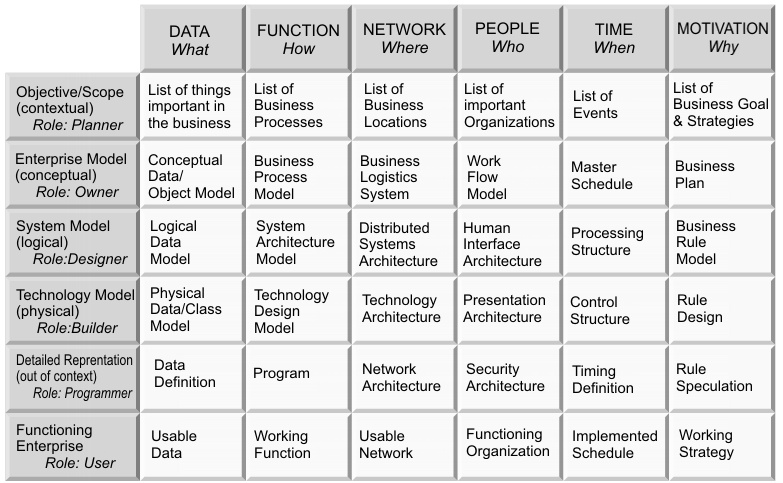
\includegraphics[width=10cm]{zachman.jpg}
    \caption{Zachmanův framework}
    \label{fig:zachman}
\end{figure}
\begin{enumerate}
\item CO? Jde zejména o informace samotné.
\item JAK? Jde o procesy prováděné s informacemi.
\item KDE? Na jakých místech se pracuje s informacemi.
\item KDO? Kdo a v jaké roli pracuje s informacemi.
\item KDY? Kdy a na základě jakých impulzů se s informacemi pracuje
\item PROČ? Jde o cíle a pravidla, jak těchto cílů dosáhnout.
\end{enumerate}
Popis rolí, artefaktů a procesů probíhajících při vývoji IS, rozdělených do vrstev podle základních otázek (co, kdo, kde, kdy, jak, proč) a úrovní granularity (high-level abstraktní pohled, low-level detailní implementační pohled)

\end{document}